% \documentclass{article}
\documentclass[a5paper]{article}

\usepackage{graphicx}
\usepackage[utf8]{inputenc}
\usepackage[margin=0.5cm]{geometry}
%  \usepackage[left=2.00cm, right=2.00cm, top=2cm, bottom=3cm]{geometry}
\usepackage{amsmath,amssymb,amsfonts}
\usepackage{soul}
\usepackage[utf8]{inputenc}
\usepackage{amssymb}
\usepackage{hyperref, xcolor}
\usepackage{cleveref}
\usepackage{multirow}   % in the preamble
\usepackage{tikz}
\usepackage{upgreek}
\hypersetup{
    colorlinks=true,
    linkcolor=[rgb]{0 0 0.5},
    urlcolor=cyan,
    citecolor= [rgb]{0 0 0.5}
}
\urlstyle{same}



\usepackage[inline]{showlabels}
\renewcommand{\showlabelfont}{\small\ttfamily\color{lightgray}} % Custom label appearance

% Ricard's edits
\newcommand{\raz}{\textcolor{purple}}



\title{Coarse-graining with Dean's method}
\author{Ashot Matevosyan}
\date{\today}


\newcommand{\la}{\left\langle}
\newcommand{\ra}{\right\rangle}
\newcommand{\bs}{\boldsymbol}
\newcommand{\E}{\mathbf{E}}
\newcommand{\Var}{\text{Var}}
\renewcommand{\d}{\mathrm{d}}
\renewcommand{\u}{\bs{u}}
\newcommand{\q}{\bs{q}}
\newcommand{\Q}{\mathbf{Q}}
\newcommand{\R}{\mathbb{R}}
\newcommand{\n}{\bs{n}}
\newcommand{\e}{\bs{e}}
\newcommand{\T}[0]{\mathrm{T}}
\newcommand{\pd}[2]{\frac{\partial #1}{\partial #2}}
\newcommand{\tpd}[2]{\tfrac{\partial #1}{\partial #2}}


\newcommand{\ab}{{\alpha\beta}}
\newcommand{\mn}{{\mu\nu}}
\newcommand{\abmn}{{\alpha\beta\mu\nu}}

\newcommand{\eye}{\bs{\mathrm{I}}}
\renewcommand{\v}{\bs{v}}
\newcommand{\x}{\mathbf{x}}
\newcommand{\f}{\mathbf{f}}
\newcommand{\s}{\mathbf{s}}
\newcommand{\g}{\mathbf{g}}
\newcommand{\G}{\mathbf{G}}
\renewcommand{\H}{\mathbf{H}}
\newcommand{\F}{\mathbf{F}}
\newcommand{\I}{\mathbf{I}}
\newcommand{\J}{\mathbf{J}}
\newcommand{\bnabla}{\boldsymbol{\nabla}}
\newcommand{\A}{\mathbf{A}}
\newcommand{\B}{\mathbf{B}}
\newcommand{\U}{\mathbf{U}}
\newcommand{\bxi}{\mathbf{\xi}}
\newcommand{\p}{\mathbf{p}}
\newcommand{\W}{\mathbf{W}}
\newcommand{\bT}{\mathbf{T}}
\newcommand{\nh}{\hat{\bs{n}}}
\newcommand{\bdelta}{\bs\delta}
\renewcommand{\ss}{\mathrm{ss}}

\newcommand{\ee}{\mathrm{e}}
\newcommand{\ii}{\mathrm{i}}

\renewcommand{\k}{\bs{k}}
\renewcommand{\r}{\mathbf{r}}

\newcommand{\TT}{{\rm T}}
\newcommand{\Tr}{{\rm T}}


\newcommand{\lM}{l_{\rm M}}
\newcommand{\lm}{l_{\rm m}}

\newcommand{\elln}{\ell_{\rm n}}
\newcommand{\ellc}{\ell_{\rm c}}
\newcommand{\elld}{\ell_{\rm d}}

\newcommand{\calN}{\mathcal{N}}
\newcommand{\calF}{\mathcal{F}}
\newcommand{\calG}{\mathcal{G}}
\newcommand{\calK}{\mathcal{K}}
\newcommand{\rmR}{\mathrm{R}}

\providecommand{\Fpair}{\calF_{\mathrm{pair}}}
\providecommand{\Fent}{\calF_{\mathrm{ent}}}
\providecommand{\Tr}{\operatorname{tr}}
\newcommand{\frev}{f_{\rm rev}}
\newcommand{\xir}{\xi_{\rm r}}
\newcommand{\ecrit}{\varepsilon_{\rm c}}
\newcommand{\sigmarho}{\sigma_\rho^2}
\newcommand{\kB}{k_\mathrm{B}}
% Correction annotations (visible in PDF)
\newcommand{\corr}[1]{\textcolor{red}{\textbf{[CORR:}\ #1\textbf{]}}}
\newcommand{\corrm}[1]{{\color{red}#1}}

\renewcommand{\div}{\text{div}}

\newcommand{\pade}{\text{pade}}

\newcommand{\Pa}{\text{Pa}}
\newcommand{\minute}{\text{min}}
\newcommand{\micron}{\upmu\mathrm{m}}

\newcommand{\ash}[1]{\textcolor{blue}{\textbf{[ash:}\ #1\textbf{]}}}




\begin{document}
\maketitle
\tableofcontents

\section*{Overview}
\begin{itemize}
    \item microscopic Langevin dynamics of self-propelled rods
    \item fluctuating dry active nematic equations
    \item activity renormalises nematic part of the free energy
    \item \textbf{Parameter choise}
    \item \textbf{Boundary conditions}
    \item steady state solution in comoving frame (defect stabilisation) using Finite Element Method (FEM)
    \item one time correlation function of the fields (density, nematic order parameter) using Lyapunov equation and Finite Difference Method (FDM)
    \item dominant effect: density fluctuations. Full analytical solution
    \item Introduction of physical small length scale cutoff.
    \item Compariosn between analytical and numerical results.
\end{itemize}

\section{Preamble}
\subsection{Model A and model B}
Coarse-grained free energy $F$ for the system.

Model A (non-conserved dynamics)

\begin{equation}\frac{\partial \rho}{\partial t}=-\frac{\delta F}{\delta \rho}+\eta(x, t)
\end{equation}

Model B (conserved dynamics)

\begin{equation}
\frac{\partial \rho}{\partial t}=\nabla^2 \frac{\delta F}{\delta \rho}+\nabla \cdot \bs\eta(x, t) .
\end{equation}
where $\eta(x, t)$ is a white noise term:
\begin{align}
    \langle \eta(x, t) \eta(x', t') \rangle = 2D \delta(x - x') \delta(t - t') \\ \langle \eta_\alpha(x, t) \eta_\beta(x', t') \rangle = 2D \delta_{\alpha\beta} \delta(x - x') \delta(t - t')
\end{align}

\subsection{Equations of active nematic}
From Ref. \cite{marchetti2013hydrodynamics}, hydrodynamic equations of active nematic are:

\begin{align}
\partial_t \rho=&-\nabla \cdot \J,
\\
\partial_t \Q=&-\frac{1}{\gamma_Q} \frac{\delta F_Q}{\delta \Q}+\f_Q
\end{align}
where the density flux is
\begin{equation}
\J=-\frac{1}{\gamma_\rho} \bnabla \frac{\delta F_Q}{\delta \rho}+\J_{\text {active}}+ \f_\rho, 
\qquad
\J_{\text {active }}=-\zeta_Q \boldsymbol{\nabla} \cdot \Q
\end{equation}
and the free energy $F_Q$ is given by:
\begin{align}
F_Q= & \int_{\mathbf{r}}\left[\frac{\alpha_Q(\rho)}{2} \mathbf{Q}: \mathbf{Q}+\frac{\beta_Q}{4}(\mathbf{Q}: \mathbf{Q})^2+\frac{K_Q}{2}(\boldsymbol{\nabla} \mathbf{Q})^2\right. \\
& \left.+C_Q \mathbf{Q}: \boldsymbol{\nabla} \boldsymbol{\nabla} \frac{\delta \rho}{\rho_0}+\frac{A}{2}\left(\frac{\delta \rho}{\rho_0}\right)^2\right]
\end{align}
THe resulting equation for the density is:
\begin{align}
    \label{density-equation-marchetti}
    \partial_t \rho=D \nabla^2 \rho+B \nabla^2 \nabla \nabla: \Q+\zeta_Q \nabla \nabla: \Q+\nabla \cdot \f_\rho,
    \\
    D=A / (\rho_0^2 \gamma_\rho), \qquad B = C_Q / (\rho_0 \gamma_\rho)
\end{align}

\section{Coarse-graining}
\subsection{Microscopic equations of motion} 

We start from the following Langevin equations governing the motion of self propelled particles \cite{cugliandolo2015,bertin2013}:
\begin{subequations}
    \label{langevin-equations}
\begin{align}
    \frac{\d\r_i}{\d t}&=\frac{\rho_0}{\xi_0}\F_i+v_0 \p_i k_i
    \label{langevin-equations-position}
    \\
    \label{langevin-equations-angle}
    \frac{\d\theta_i}{\d t}&=\frac{\rho_0}{\xir}\Gamma_i+\lambda_i
\end{align}
\end{subequations}
These are already overdamped equations of motion.
$\r_i$ is the position of the particle $i$, $\theta_i$ is the angle of the particle $i$ with 
\begin{align}
    \p_i = (\cos \theta_i, \sin \theta_i)^T,
    \qquad
    \label{Q-unit-def}
    \hat\Q(\theta) = 
    2 \p(\theta)\p(\theta) - \I =  \begin{pmatrix}
        \cos 2\theta & \sin 2\theta
        \\
        \sin 2\theta & -\cos 2\theta
    \end{pmatrix}
\end{align}
being the unit vector in the direction of the particle $i$. $\xi_0/\rho_0$ and $\xir/\rho_0$ are the friction coefficients. $\rho_0$ is the reference density, we include this factor for later convenience.
$\F_i$ is the force acting on the particle $i$, $\Gamma_i$ is the torque acting on the particle $i$. $\lambda_i$ is a white noise of the rotation.
For simplicity, we assume $\theta_i \in \mathbb{R}$ and $\theta_i$ and $\theta_i+2\pi$ are the same directional state of the particle $i$. Therefore, we also use 
\begin{equation}
    \la \lambda_i(t) \lambda_j(t') \ra = 2 \Lambda \delta_{ij} \delta(t-t')
\end{equation}
where $\delta_{ij}$ is the Kronecker delta, $\delta(t-t')$ is the Dirac delta function, and $\Lambda$ is the intensity of the noise.

The last term in \cref{langevin-equations-position} is the self propulsion term in the direction of $\p_i$ with speed $v_0$. $k_i$ is a dichotomous noise and takes the values $1$ and $-1$ with equal probability. It models the random reversal of the direction of the particle $i$ with rate $\frev$. Therefore, we have the following autocorrelation function for $k_i$:
\begin{equation}
    \label{k-autocorrelation}
    \la k_i(t) k_j(t') \ra = \delta_{ij}\ee^{-2 \frev |t-t'|}
\end{equation}
We are interested in the dynamics at larger time scales than the reversal time $\frev^{-1}$. Therefore, we can approximate the dichotomous noise $k_i$ as a continuous gaussian white noise:
\begin{equation}
    \label{k-approximation}
    \la k_i(t) k_j(t') \ra \approx \frev^{-1} \delta_{ij} \delta(t-t')
\end{equation}
This approximation will be useful in the following calculations.
The forces and torques are derived from the total potential energy:
\begin{align}
    V_\text{total}(\r_1, \theta_1, \r_2, \theta_2, \ldots, \r_N, \theta_N) = \frac{1}{2}\sum_{i,j=1}^N V(\r_i-\r_j, \theta_i, \theta_j)
\end{align}
where $V(\x, \theta, \theta')$ is the pairwise interaction potential. It obeys the exchange symmetry $V(\r-\r',\theta, \theta') = V(\r-\r',\theta', \theta)$ and, by Newton's third law, $V(\r-\r',\theta, \theta') = V(\r'-\r,\theta', \theta)$.
Therefore, the forces and torques are
\begin{align}\label{F-field-def}
    \F_i = \F(\r_i, \theta_i) \qquad \Gamma_i = \Gamma(\r_i, \theta_i)
\end{align}
where
\begin{align}
    \label{F-definition}
    \F(\r,\theta) = -\sum_{j=1}^{N}
    \pd{}{\r} V(\r-\r_j, \theta, \theta_j)
    \qquad
    \Gamma(\r,\theta) = -\sum_{j=1}^{N}
    \pd{}{\theta} V(\r-\r_j, \theta, \theta_j)
\end{align}


\subsection{Dean's approach}
Now we apply the Dean's approach \cite{dean1996} to derive a langevin euqation for the density field. 
Define the density of the $i$-th particle as
\begin{align}
    \label{rho-i-definition}
    \varrho^{(i)}_t(\r, \theta) = \delta(\r-\r_i(t)) \delta(\theta-\theta_i(t))
\end{align}
Then the density (over the state space) is given by
\begin{align}
    \label{varrho-definition}
    \varrho_t(\r, \theta) = \frac{1}{\rho_0}\sum_{i=1}^N \varrho^{(i)}_t(\r, \theta)
\end{align}
Here, $\rho_0$ is the reference density, which makes $\varrho_t$ dimensionless.
Assuming $\nabla V(\r,\theta,\theta')$ vanishes at $\r=0$ (so that a particle exerts no force on itself), we can write the force and torque in terms of the density field as
\begin{align}
    \label{F-rho}
    \F(\r,\theta) =& -\pd{}{\r}\int \d\r' \d\theta' 
    V(\r-\r', \theta, \theta') \rho_0\,\varrho_t(\r', \theta') 
    \\ 
    \Gamma(\r,\theta) =& -\pd{}{\theta}\int \d\r' \d\theta' 
    V(\r-\r', \theta, \theta') \rho_0\,\varrho_t(\r', \theta') 
\end{align}
and the force and torque acting on the $i$-th particle are given by $\F_i = \F(\r_i, \theta_i)$ and $\Gamma_i = \Gamma(\r_i, \theta_i)$.

For any test function $f(\r, \theta)$, we can write
\begin{align}
    f(\r_i(t), \theta_i(t)) = \int \d\r \d\theta f(\r, \theta) \varrho^{(i)}_t(\r, \theta)
\end{align}
Now, taking the total time differential:
\begin{align}
    \d f(\r_i, \theta_i) 
    =& \pd{f(\r_i, \theta_i)}{r_{i,\alpha}} \d r_{i,\alpha}
    + \frac{1}{2} \frac{\partial^2 f(\r_i, \theta_i)}{\partial r_{i,\alpha}\partial r_{i,\beta}}
    \d r_{i,\alpha}\d r_{i,\beta}
    \\
    &+ \pd{f(\r_i, \theta_i)}{\theta_i} \d\theta_i
    + \frac{1}{2} \frac{\partial^2 f(\r_i, \theta_i)}{\partial \theta_i^2} \d\theta_i\d\theta_i
\end{align}
Now, we substitute the Langevin equations \eqref{langevin-equations} and \cref{F-field-def}. We only keep the terms untill first order in $\d t$. For example, $ (\lambda_i \d t)^2 = 2\Lambda \d t$ and $ (k_i\d t)^2 = \frev^{-1} \d t$:
\begin{align}
    \label{total-time-derivative-f}
    \frac{\d}{\d t} f(\r_i(t), \theta_i(t)) 
    =& \pd{f(\r_i, \theta_i)}{\r_i} \cdot\left( \frac{\rho_0}{\xi_0}\F(\r_i, \theta_i) + v_0 \p(\theta_i) k_i \right) + \pd{f(\r_i, \theta_i)}{\theta_i} \left( \frac{\rho_0}{\xir}\Gamma(\r_i, \theta_i) + \lambda_i \right) 
    \\
    &+ \frac{\zeta}{\xi_0} 2 p_\alpha(\theta_i) p_\beta(\theta_i) \frac{\partial^2 f(\r_i, \theta_i)}{\partial r_{i,\alpha}\partial r_{i,\beta}} 
    + \Lambda \frac{\partial^2 f(\r_i, \theta_i)}{\partial \theta_i^2}
\end{align}
where we defined
\begin{align}
    \zeta = \frac{\xi_0 v_0^2}{4\frev}
\end{align}
This will end up being active stress coefficient.
We can rewrite this in terms of the one particle density field:
\begin{align}
    \frac{\d}{\d t} f =& \int \d\r \d\theta \varrho^{(i)}_t(\r, \theta) \left[
        \pd{f(\r, \theta)}{\r}\cdot \left(\frac{\rho_0}{\xi_0}\F(\r, \theta) + v_0 \p(\theta) k_i\right) + \pd{f(\r, \theta)}{\theta} \left(\frac{\rho_0}{\xir}\Gamma(\r, \theta) + \lambda_i\right)
    \right.
    \\
    &\qquad\qquad\qquad\qquad\left.
        + \frac{\zeta}{\xi_0} 2 p_\alpha(\theta) p_\beta(\theta) \frac{\partial^2 f(\r, \theta)}{\partial r_{\alpha}\partial r_{\beta}} 
    + \Lambda \frac{\partial^2 f(\r, \theta)}{\partial \theta^2}
    \right]
\end{align}
Now, by integration by parts, we can obtain
\begin{align}
    \frac{\d}{\d t} f =& \int \d\r \d\theta f( \r, \theta) \left[-
    \pd{}{\r} \cdot\left( \varrho^{(i)}_t(\r, \theta) \left(\frac{\rho_0}{\xi_0}\F(\r, \theta) + v_0 \p(\theta) k_i\right) \right)
    \right.
    \\
    &\qquad\qquad\qquad\quad
    -\pd{}{\theta} \left( \varrho^{(i)}_t(\r, \theta) \left(\frac{\rho_0}{\xir}\Gamma(\r, \theta) + \lambda_i\right) \right)
    \\
    &\qquad\qquad\qquad\quad\left.
        + \frac{\zeta}{\xi_0} 2 p_\alpha(\theta) p_\beta(\theta) \frac{\partial^2 \varrho^{(i)}_t(\r, \theta)}{\partial r_{\alpha}\partial r_{\beta}} 
    + \Lambda \frac{\partial^2 \varrho^{(i)}_t(\r, \theta)}{\partial \theta^2}
    \right]
\end{align}
On the other hand, we can also write $\frac{\d}{\d t} f = \int \d\r \d\theta f(\r, \theta)\pd{}{t}\varrho^{(i)}_t(\r, \theta) $. Note that $f$ is an arbitrary test function, therefore we have the following relation:
\begin{align}
    \pd{}{t}\varrho^{(i)}_t(\r, \theta) =& -
    \pd{}{\r}\cdot \left( \varrho^{(i)}_t(\r, \theta) \left(\frac{\rho_0}{\xi_0}\F(\r, \theta) + v_0 \p(\theta) k_i\right) \right)
    -
    \pd{}{\theta} \left( \varrho^{(i)}_t(\r, \theta) \left(\frac{\rho_0}{\xir}\Gamma(\r, \theta) + \lambda_i\right) \right)
    \\
    &+ \frac{\zeta}{\xi_0} 2 p_\alpha(\theta) p_\beta(\theta) \frac{\partial^2 \varrho^{(i)}_t(\r, \theta)}{\partial r_{\alpha}\partial r_{\beta}} 
    + \Lambda \frac{\partial^2 \varrho^{(i)}_t(\r, \theta)}{\partial \theta^2}
\end{align}
Now, summing over all particles, we get
\begin{align}
    \pd{}{t}\varrho_t(\r, \theta) =& 
    \left[-\frac{\rho_0}{\xi_0}\pd{}{\r}\cdot\left(\varrho_t(\r, \theta)\F(\r, \theta)\right)
    -
    \frac{\rho_0}{\xir}\pd{}{\theta} \left(\varrho_t(\r, \theta)\Gamma(\r, \theta)\right)
    \right]
    \\
    &+
    \left[\frac{\zeta}{\xi_0} 2 p_\alpha(\theta) p_\beta(\theta) \frac{\partial^2 \varrho_t(\r, \theta)}{\partial r_{\alpha}\partial r_{\beta}} 
    + \Lambda \frac{\partial^2 \varrho_t(\r, \theta)}{\partial \theta^2}
    \right]
    \\
    &-
    \sum_{i=1}^N\frac{1}{\rho_0}\left[
     \pd{}{\r}\cdot\left( v_0 \p(\theta) \varrho^{(i)}_t(\r, \theta) k_i(t)\right) +  \pd{}{\theta}\left( \varrho^{(i)}_t(\r, \theta)\lambda_i(t) \right)
    \right]
\end{align}
Recall the factor $\rho_0^{-1}$ in \cref{varrho-definition}.
Here, the second line is the noise term and it still depends on the individual particle densities. We will deal with it later.
For the deterministic part, we define a free energy functional as
\begin{align}
    \label{free-energy-functional-definition}
    \mathcal{F}[\varrho] = \frac{1}{2}\int \d\r \d\r'\d\theta \d\theta' \rho_0^2\varrho(\r, \theta) \varrho(\r', \theta') V(\r-\r', \theta, \theta')
\end{align}
The variational derivative of the free energy functional is a function of $\r$ and $\theta$ and has dimension of energy density:
\begin{align}
    \frac{\delta\calF}{\delta\varrho(\r, \theta)} = \int \d\r' \d\theta' \rho_0^2 \varrho(\r', \theta') V(\r-\r', \theta, \theta')
\end{align}
Note that the force and torque fields in \cref{F-rho} can be written as $\F(\r, \theta) = -\frac{1}{\rho_0}\pd{}{\r}\frac{\delta\calF}{\delta\varrho(\r, \theta)}$ and $\Gamma(\r, \theta) = -\frac{1}{\rho_0} \pd{}{\theta}\frac{\delta\calF}{\delta\varrho(\r, \theta)}$.
Thus
\begin{align}
    \pd{}{t}\varrho_t(\r, \theta) =& 
    \frac{1}{\xi_0}\pd{}{\r}\cdot\left(\varrho_t(\r, \theta)\pd{}{\r}\frac{\delta\calF}{\delta\varrho}\right)
    +\frac{1}{\xir}\pd{}{\theta}\left(\varrho_t(\r, \theta)\pd{}{\theta}\frac{\delta\calF}{\delta\varrho}\right)
    \\
    &
    +\text{active}
   +\text{noise}
\end{align}

Next, we represent the noise term in terms of particle independent variables. Note that the translational and rotational noise are independent, thus we study them independently.
consider the following autocorrelation function of the $\f(\r, \theta, t) = \sum_i \rho_0^{-1} v_0\varrho^{(i)}_t(\r, \theta) \p(\theta) k_i(t)$:
\begin{align}
    \langle f_\alpha(\r, \theta, t) &f_\beta(\r', \theta', t') \rangle = \sum_{i,j=1}^N (v_0/\rho_0)^2 \varrho^{(i)}_t(\r, \theta) \varrho^{(j)}_{t'}(\r', \theta') p_\alpha(\theta) p_\beta(\theta') \la k_i(t) k_j(t') \ra
    \\
    =& \sum_{i}^N (v_0/\rho_0)^2 \varrho^{(i)}_t(\r, \theta) \varrho^{(i)}_{t'}(\r', \theta') p_\alpha(\theta) p_\beta(\theta') ~\frev^{-1}\delta(t-t')
    \\
    =& \sum_{i}^N (v_0/\rho_0)^2 \varrho^{(i)}_t(\r, \theta) \delta(\r-\r') \delta(\theta-\theta') p_\alpha(\theta) p_\beta(\theta')~\frev^{-1}\delta(t-t')
    \\
    =& \frac{v_0^2}{\frev \rho_0} \varrho_t(\r, \theta) p_\alpha(\theta) p_\beta(\theta) \delta(t-t')\delta(\r-\r') \delta(\theta-\theta')
\end{align}
Here, we used \cref{k-autocorrelation} in the second line. In the third line we expanded the single particle density (c.f.~\cref{rho-i-definition}) and used the fact that $\delta(\r - \r_i)\delta(\r'-\r_i) = \delta(\r - \r_i)\delta(\r - \r')$ etc. 
So let's define a random noise field $k(\r, \theta, t)$ so that the autocorrelation function of it is given by
\begin{align}
    \la k(\r, \theta, t) k(\r', \theta', t') \ra = \frac{4\zeta}{\xi_0\rho_0} \delta(t-t') \delta(\r-\r') \delta(\theta-\theta')
\end{align}
and for the translational noise we get $\f(\r, \theta, t) = \sqrt{\varrho_t(\r, \theta)} \p(\theta) k(\r, \theta, t)$.

Similarly, for the rotational noise, let $g(\r, \theta, t) = \sum_i \rho_0^{-1}\varrho^{(i)}_t(\r, \theta) \lambda_i(t)$. The autocorrelation function of it is given by
\begin{align}
    \la g(\r, \theta, t) g(\r', \theta', t') \ra =& \sum_{i,j=1}^N \frac{1}{\rho_0^2}\varrho^{(i)}_t(\r, \theta) \varrho^{(j)}_{t'}(\r', \theta') \la \lambda_i(t) \lambda_j(t') \ra
    \\
    =& \sum_{i}^N \frac{1}{\rho_0^2}\varrho^{(i)}_t(\r, \theta) \delta(\r-\r') \delta(\theta-\theta') 2 \Lambda \delta_{ij} \delta(t-t')
    \\
    =& \varrho_t(\r, \theta) \frac{2 \Lambda}{\rho_0} \delta(t-t') \delta(\r-\r') \delta(\theta-\theta')
\end{align}
So let's define a random noise field $\lambda(\r, \theta, t)$ so that the autocorrelation function of it is given by
\begin{align}
    \la \lambda(\r, \theta, t) \lambda(\r', \theta', t') \ra = \frac{2 \Lambda}{\rho_0} \delta(t-t') \delta(\r-\r') \delta(\theta-\theta')
\end{align}
and for the rotational noise we get $g(\r, \theta, t) = \sqrt{\varrho_t(\r, \theta)} \lambda(\r, \theta, t)$.


Finally, we get a closed Langevin equation for the density field:
\begin{equation}
\boxed{
\begin{aligned}
    \label{final-langevin}
    \pd{}{t}\varrho_t(\r, \theta) = &
    \frac{1}{\xi_0}\pd{}{\r}\cdot\left(\varrho_t(\r, \theta)\pd{}{\r}\frac{\delta\calF}{\delta\varrho}\right)
    +\frac{1}{\xir}\pd{}{\theta}\left(\varrho_t(\r, \theta)\pd{}{\theta}\frac{\delta\calF}{\delta\varrho}\right)
    \\
    &+\frac{\zeta}{\xi_0} 2 p_\alpha(\theta) p_\beta(\theta) \frac{\partial^2 \varrho_t(\r, \theta)}{\partial r_{\alpha}\partial r_{\beta}} 
    + \Lambda \frac{\partial^2 \varrho_t(\r, \theta)}{\partial \theta^2}
    \\
        &- \pd{}{\r}\cdot\left(\sqrt{\varrho_t(\r, \theta)}\p(\theta) k(\r, \theta, t)\right)
        - \pd{}{\theta}\left(\sqrt{\varrho_t(\r, \theta)} \lambda(\r, \theta, t)\right)
\end{aligned}
}
\end{equation}


Few remarks before we move on:
\begin{itemize}
    \item $\varrho_t(\r, \theta)$ is a distribution over the state space. Ussially, we are interested in it's marginal distributions $\rho_t(\r)$ and it's moments over angular variable $\theta$ (first and second moments for polar and nematic order parameters respectively). In the current form, it is impossible to obtain closed equations for these observable quantities. In the following section, we will consider a specific form of the free for which we will be able to obtain the closed equations.
    \item The noise in the angular langevin euqation ends up as a entropy term in the free energy functional. Later on, we will see that it renormalizes the free energy.
\end{itemize}

\subsection{Choosing the free energy functional}
Let's assume that the free energy functional depends on the density and the nematic order parameter, and depends on the full density implicitly through them \footnote{
Microscopic definition of the nematic order parameter is $\Q(\r) =\frac{1}{\rho(\r)} \int \d\theta \varrho(\r, \theta) \hat\Q(\theta)$, however, later we are going to consider the limit of incompressible monolayer with density $\rho_0$, in which case $\rho(\r) = 1$. On the other hand, this can be viewed as our choice of parametrization of the free energy functional}:
\begin{align}
    \calF = F[\rho, \Q]
    \\
    \rho(\r) = \int \d\theta \varrho(\r, \theta),\qquad \Q(\r) = \int \d\theta \varrho(\r, \theta) \hat\Q(\theta)
\end{align}
Note that $\rho(\r)$ is the density field scaled by the reference density $\rho_0$.
Then, the variational derivative of the free energy functional is given by:
\begin{align}
    \frac{\delta\calF}{\delta\varrho(\r, \theta)} = \int \d\r' \left[
        \frac{\delta F}{\delta \rho(\r')} \frac{\delta \rho(\r')}{\delta\varrho(\r, \theta)} + \frac{\delta F}{\delta \Q(\r')} \frac{\delta \Q(\r')}{\delta\varrho(\r, \theta)}
    \right]
\end{align}
Next, we compute the variational derivatives of $\rho(\r)$ and $\Q(\r)$:
\begin{align}
    \frac{\delta \rho(\r')}{\delta\varrho(\r, \theta)} =& \int \d\theta' \frac{\delta \varrho(\r', \theta')}{\delta\varrho(\r, \theta)} = \delta(\r-\r') 
    \\
    \frac{\delta \Q(\r')}{\delta\varrho(\r, \theta)}=& 
    \int \d\theta' \hat\Q(\theta') \frac{\delta \varrho(\r', \theta')}{\delta\varrho(\r, \theta)}
    = \hat\Q(\theta)\delta(\r-\r') 
\end{align}
Using this, we get
\begin{align}
    \frac{\delta\calF}{\delta\varrho(\r, \theta)} = \frac{\delta F}{\delta \rho(\r)}  + \frac{\delta F}{\delta \Q(\r)} : \hat\Q(\theta) 
\end{align}


\subsection{Integrating out the angle}
\subsubsection{Density equation}
Now, we integrate the \cref{final-langevin} over the angle $\theta$. Integrate term by term:
\begin{align}
&\int \d\theta
    \varrho(\r, \theta)\partial_\r \frac{\delta \calF}{\delta \varrho(\r, \theta)}
    =
        \int \d\theta \varrho(\r, \theta)\partial_\r \left(\frac{\delta F}{\delta \rho(\r)} 
        + \frac{\delta F}{\delta \Q(\r)} : \hat\Q(\theta) 
        \right)
    \\
    &=\rho \partial_\r \frac{\delta F}{\delta \rho}
    +\Q(\r):\partial_\r\frac{\delta F}{\delta \Q(\r)} 
\end{align}
\begin{align}
    &\int \d\theta \partial_\theta\left(\varrho_t(\r, \theta)\partial_\theta\frac{\delta\calF}{\delta\varrho}\right) = 0
    \qquad
    \int \d\theta\Lambda \frac{\partial^2 \varrho(\r, \theta)}{\partial \theta^2} = 0
    \\
    &\int \d\theta 2 \p(\theta) \p(\theta) :\partial_\r\partial_\r \varrho_t(\r, \theta) 
    = \int \d\theta \hat\Q(\theta):\partial_\r\partial_\r \varrho_t(\r, \theta) + \int \d\theta \nabla^2 \varrho_t(\r, \theta)
    \\
    &\qquad=\left(\partial_\r\partial_\r : \Q + \nabla^2 \rho\right)
\end{align}
Putting everything together, we get
\begin{align}
    \label{rho-equation}
    \boxed{
    \partial_t \rho = \frac{1}{\xi_0}\partial_\r \cdot\left(
    \rho \partial_\r \frac{\delta F}{\delta \rho}\right)
    + \frac{1}{\xi_0} \partial_\r \cdot\left( \Q:\partial_\r \frac{\delta F}{\delta \Q}\right)
    + \frac{\zeta}{\xi_0} \left(\nabla^2 \rho + \partial_\r\partial_\r : \Q\right)
    + 
    f_\rho(\r, t)
    }
\end{align}
where $f_\rho(\r, t)$ is a noise term:
\begin{align}
    f_\rho(\r, t) = \int \d\theta \left[-
    \pd{}{\r}\cdot\left(\sqrt{\varrho_t(\r, \theta)} \p(\theta) k(\r, \theta, t)\right)
    - \pd{}{\theta}\left(\sqrt{\varrho_t(\r, \theta)} \lambda(\r, \theta, t)\right)
    \right]
\end{align}
It's autocorrelation function is given by:
\begin{align}
    \label{rho-noise-autocorrelation}
    \la f_\rho(\r, t) f_\rho(\r', t') \ra =& \delta(t-t')
    \int \d\theta 
    \partial_\alpha\partial'_\beta\left[
    \varrho_t(\r, \theta) \frac{2\zeta}{\xi_0\rho_0} \left(\hat Q_\ab(\theta)+\delta_\ab\right)\delta(\r-\r')\right]
    \\
    =&\frac{2\zeta}{\xi_0\rho_0} \delta(t-t') 
    \frac{\partial^2}{\partial r_\alpha \partial r'_\beta}\left[(Q_\ab(\r)+\rho(\r) \delta_\ab)
   \delta(\r-\r')\right]
\end{align}
The noise from the angular langevin equation has no contribution here.
 


Now, we multiply \cref{final-langevin} by $\hat\Q(\theta)$, then integrate over $\theta$:
\begin{align}
    \partial_t \Q =& 
    \frac{1}{\xi_0}\partial_\r \cdot\left(\Q \partial_\r \frac{\delta F}{\delta \rho}\right)
    +\frac{1}{\xi_0}\partial_\r \cdot\left(
        \int \d\theta \varrho(\r, \theta) \hat\Q(\theta) \hat\Q(\theta) : \partial_\r \frac{\delta F}{\delta \Q}\right)
\\    
    &-\frac{1}{\xir}\int \d\theta \varrho(\r, \theta) \hat\Q'(\theta)\hat\Q'(\theta) : \frac{\delta F}{\delta \Q}-4\Lambda \Q
    \\
    &+\frac{\zeta}{\xi_0}\nabla^2 \Q + \frac{\zeta}{\xi_0} \partial_\r\partial_\r : \int \d\theta \varrho(\r, \theta) \hat\Q(\theta) \hat\Q(\theta)
\end{align} 

We use the following closure approximation, which holds when nematic order strength $S\ll 1$:
\begin{align}
    \int \d\theta \varrho(\r, \theta) \hat\Q(\theta) \hat\Q(\theta) = \rho \J
    \\
    \int \d\theta \varrho(\r, \theta) \hat\Q'(\theta)\hat\Q'(\theta) = 4\rho \J
\end{align}
where $J_{\abmn} =\frac{1}{2}\left(\delta_{\alpha\mu}\delta_{\beta\nu} + \delta_{\alpha\nu}\delta_{\beta\mu} - \delta_{\alpha\beta}\delta_{\mu\nu}\right)$ is rank-4 identity tensor:
\begin{align}
    \J:\Q  = \Q,
    \qquad
    \J : \partial_\r\partial_\r  = 
    \partial_\r\partial_\r -\frac{1}{2}\I \nabla^2
\end{align}
Then, we end up

\begin{equation}
\label{Q-equation}
\boxed{
\begin{aligned}
    \partial_t \Q =& 
    \frac{1}{\xi_0}\partial_\r \cdot\left(\Q \partial_\r \frac{\delta F}{\delta \rho}\right)
    +\frac{1}{\xi_0}\partial_\r \cdot\left(\rho\partial_\r \frac{\delta F}{\delta \Q}\right)
    -\frac{4\rho}{\xir}\frac{\delta F}{\delta \Q} -4\Lambda \Q
    \\
    &+\frac{\zeta}{\xi_0}\left(\partial_\r\partial_\r \rho + \nabla^2 \left(\Q -\tfrac{1}{2}\I \rho\right) \right) + \f^Q(\r, t)
\end{aligned}
}
\end{equation}
where $\f^Q(\r, t)$ is a noise term:
\begin{align}
    \f^Q(\r, t) =\int \d\theta \hat\Q(\theta) \left[-
    \pd{}{\r}\cdot\left(\sqrt{\varrho_t(\r, \theta)} \p(\theta) k(\r, \theta, t)\right)
    - \pd{}{\theta}\left(\sqrt{\varrho_t(\r, \theta)} \lambda(\r, \theta, t)\right)
    \right]
\end{align}
It's autocorrelation function is given by:
\begin{align}
    \label{Q-noise-autocorrelation}
    &\la f^Q_\ab(\r, t) f^Q_\mn(\r', t') \ra = 
    \delta(t-t') \delta(\r-\r') \frac{2\Lambda}{\rho_0} \la \hat Q'_\ab \hat Q'_\mn\ra_{\varrho(\r)}
    \\
    &\hspace{1cm}+\delta(t-t')\frac{2\zeta}{\xi_0\rho_0} 
    \frac{\partial^2}{\partial r_i \partial r'_j}\left[\left(
        \la \hat Q_\ab \hat Q_\mn \hat Q_{ij}\ra_{\varrho(\r)}
        +\la \hat Q_\ab \hat Q_\mn\ra_{\varrho(\r)} \delta_{ij}
    \right)\delta(\r-\r')
    \right]
\end{align}
Here, we defined couple of moments:
\begin{align}
    \la \hat Q_\ab \hat Q_\mn \hat Q_{ij}\ra_\varrho =& \int\d\theta \varrho_t(\r, \theta) \hat Q_\ab(\theta) \hat Q_\mn(\theta) \hat Q_{ij}(\theta) 
    \\
    \la \hat Q_\ab \hat Q_\mn\ra_\varrho =& \int\d\theta \varrho_t(\r, \theta) 
    \hat Q_\ab(\theta) \hat Q_\mn(\theta)
    \\
    \la \hat Q'_\ab \hat Q'_\mn\ra_\varrho =& \int\d\theta \varrho_t(\r, \theta) \hat Q'_\ab(\theta) \hat Q'_\mn(\theta)
\end{align}
where $\hat Q'_\ab(\theta) = \pd{\hat Q_\ab(\theta)}{\theta}$. In \cref{max-entropy-moments} we computed these moments up to $S^2$ order.

Remains to calculate the cross-autocorrelation function of the noise terms:
\begin{align}
    \label{noise-cross-autocorrelation}
    \la f^Q_\ab(\r, t) f_\rho(\r', t') \ra = \delta(t-t')\frac{2\zeta}{\xi_0\rho_0} \frac{\partial^2}{\partial r_i \partial r'_j}\left[
        \left(\la \hat Q_\ab \hat Q_{ij} \ra_{\varrho(\r)} + Q_\ab(\r) \delta_{ij}\right)
        \delta(\r-\r')
    \right]
\end{align}
\section{System of interest: Myxobacteria monolayer}
First assumption that we make is that the monolayer is incompressible. We will model it with high bulk modulus of compressibility. Therefore, the monolayer density $\rho$ will have small variation around $\rho_0$.


Let the free energy of the system be given by
\begin{align}
    \label{free-energy-choice}
    &F[\rho, \Q] =\int \d\r \;\mathfrak{f}(\rho(\r), \Q(\r))
    \\
    \label{free-energy-choice-2}
    &\mathfrak{f}(\rho,\Q)= 
    \frac{B}{2}\left(\rho-1\right)^2 + \frac{a}{2}(\Q:\Q) + \frac{b}{4}(\Q:\Q)^2 + \frac{K}{2}(\partial_\r \Q):(\partial_\r \Q)
\end{align}
where $\mathfrak{f}$ is the free energy density (note the units are $\text{Pa} \cdot \micron$).
The first part of $\mathfrak{f}$ models the incompressibility of the monolayer with bulk modulus $B \gg 1$. The second part is the free energy of the nematic interaction.

\subsection{Parameter choice}
\label{sec-parameter-choice}
In Ref. \cite{copenhagen}, the following parameters were estimated from experiments:

\begin{tabular}{|l|l|l|l|}
    \hline Parameter & +1/2 defects & -1/2 defects & Joint fit 
    \\ \hline 
    $\elld~(\micron)$ & $2.5 \pm 0.1$ & $2.54 \pm 0.02$ & $2.55\pm 0.07$ 
    \\ \hline 
    $\zeta / \xi_0\left(\micron^2 / \mathrm{min}\right)$ & $1.77 \pm 0.09$ & $4.65 \pm 0.04$ 
    & $2.09 \pm 0.07$
    \\ \hline 
    $\epsilon$ & $0.80 \pm 0.01$ & $0.214 \pm 0.006$ 
    & $0.77 \pm 0.01$
    \\ \hline
    $S_0$ & \multicolumn{3}{c|}{$0.992\pm 0.003$}
    \\ \hline
\end{tabular}\linebreak
where $\epsilon$ is the friction anisotropy coefficient, $\elld$ is the defect core size. For the passive system\footnote{As we will see later,for active system the free energy parameters are renormalized due to activity.} these are related to the free energy parameters as:
\begin{align}
    \label{dcsos}
    \elld = \sqrt{K/(-a)} \qquad S_0 = \sqrt{-a/(2b)}
\end{align}

In Ref. \cite{han2025local}, we find another set of parameters:

\noindent
\begin{tabular}[t]{|l|l|}
    \hline Parameter & +1/2 defects  
    \\ \hline 
    $\elld~(\micron)$ & $0.8$ 
    \\ \hline 
    $\epsilon$ & $0.35$
    \\ \hline 
    $S_0$ & $1.2$
    \\ \hline
    $R ~(\micron)$ & $10$
    \\ \hline
\end{tabular}
\hspace{1cm}
\begin{tabular}[t]{|l|l|}
    \hline Parameter & +1/2 defects
    \\ \hline
    $\xi_0 ~\left(\text{Pa} \cdot \text{min} / \micron\right)$ & $6.5$
    \\ \hline 
    $\zeta~ \left(\text{Pa} \cdot \micron\right)$ & $3.8$
    \\ \hline
    $\frev~\left(\text{min}^{-1}\right)$ & $0.1$
    \\ \hline
    $v_0~\left(\micron / \text{min}\right)$ & $1$
    \\ \hline
    $\rho_0~\left(\micron^{-2}\right)$ & $0.3$
    \\ \hline
\end{tabular}

In this case, the nematic order strength $S_0$ was decaying to zero with exponential decay with radius $R$.


% The our definition of $\xi_0$ and $\zeta$ is different from the one in Refs. \cite{han2025local,copenhagen}. For example, they have $\xi_0 \v$ as force density (units of Pa), while $\xi_0 \v$ is a force according to \eqref{langevin-equations}. Two definitions are different by a factor of $\rho_0$.

Now we present our choice of parameters. We list them in three groups.
First, the ``known'' parameters that we get from the experimental data:
\begin{gather}
    \rho_0 = 0.3 ~\micron^{-2},
    \quad
    \xi_0 = 5 ~\Pa \cdot \minute / \micron,
    \quad
    \zeta = 8 ~\Pa \cdot \micron,
    \\
    \quad
    \elld = 1 ~\micron,
    \quad
    S_0 = 0.9,
    \quad
    \epsilon = 0,
\end{gather}
We do not consider unisotropic friction in our model, setting $\epsilon = 0$.
For the defect core size we follow Ref.~\cite{han2025local}, which gives $\elld \simeq 1~\micron$, rather than the larger $\elld = 2.5 \pm 0.1~\micron$ of Ref.~\cite{copenhagen}; the remaining entries of this group are taken from Ref.~\cite{copenhagen} and from our own estimates, so the set is deliberately mixed.
The next group is the parameters that we guess:
\begin{gather}
    B = 2\cdot10^{5} ~\Pa \cdot \micron,
    \quad
    \gamma = 8 ~\minute^{-1},
    \quad
    \Lambda = 0.1 ~\minute^{-1},
\end{gather}
Here, $\gamma$ is the relaxation rate of the nematic order parameter. (Not to be confused with the surface tension of \cref{sec-extrusion}, for which we reserve $\gamma_{\rm w}$, nor with $\gamma_0 = B/\xi_0 = 4\cdot10^{4}~\micron^2/\minute$, the density relaxation coefficient of \eqref{eq:sde}.)
If we impose Fluctuation-Dissipation Theorem on the rotational diffusion coefficient $\Lambda$ in \cref{langevin-equations-angle}, then
\begin{align}
    \Lambda = \frac{\kB T}{(\xir/\rho_0)}
\end{align}
Here, $\kB T = 4.1 \cdot 10^{-3} ~\Pa \cdot \micron^3$ and $\Lambda \xi_0 \approx 10^{-2} ~\Pa \cdot \micron$. This makes $\xir=0.1 ~\Pa \cdot \micron \cdot \minute$.
Then we use the following relations to get the rest of the model parameters:
\begin{align}
    \elld = \sqrt{(K+\zeta\xir/(4\xi_0))/(-a-\Lambda \xir)} \qquad S_0 = \sqrt{-(a+\Lambda \xir)/(2b)}
    \qquad 
     \gamma = {8 b}/{\xir}
\end{align}
The first two are \eqref{dcsos}, where the free energy parameters are renormalized due to activity, more on this in \cref{sec-noiseless-dynamics}. 
We derive the third one in \cref{app-Q-relaxation}.
Then, for the model parameters we infer the following values:
\begin{gather}
    \rho_0 = 0.3 ~\micron^{-2},
    \qquad
    B = 2\cdot10^{5} ~\Pa \cdot \micron,
    \qquad
    \\
    a = -0.172 ~\Pa \cdot \micron,
    \qquad
    b = 0.1 ~\Pa \cdot \micron,
    \qquad
    K = 0.122 ~\Pa \cdot \micron^3,
    \\
    \zeta = 8 ~\Pa \cdot \micron,
    \qquad
    \xi_0 = 5 ~\Pa \cdot \minute / \micron,
    \qquad
    \xir = 0.1 ~\Pa \cdot \micron \cdot \minute,
    \quad
    \Lambda = 0.1 ~\minute^{-1},
\end{gather}
These are the \emph{bare} free-energy parameters, i.e.\ the $a$, $b$, $K$ that solve \eqref{dcsos-renormalized}; the activity-renormalised combinations that actually set the defect structure are
\begin{align}
    \label{primed-values}
    a' = a + \Lambda \xir = -0.162 ~\Pa \cdot \micron,
    \qquad
    b' = b,
    \qquad
    K' = K + \frac{\zeta\xir}{4\xi_0} = 0.162 ~\Pa \cdot \micron^3,
\end{align}
from which $\elld = \sqrt{K'/(-a')} = 1~\micron$ and $S_0 = \sqrt{-a'/(2b')} = 0.9$ as required. It is worth keeping the primes visible: $a'$ is fixed by $S_0$ and $b$ alone and so does not move when $\elld$ is changed, whereas $K$ and $K'$ both do.


$k_B T = 4.1 \cdot 10^{-3} ~\Pa \cdot \micron^3$
and the rotational diffusion coefficient $\Lambda$ in thermal equilibrium is given by $\Lambda = \rho_0 k_B T / \xi_0$



\subsection{Noiseless dynamics}
\label{sec-noiseless-dynamics}
In this section we will drop the noise terms $f_\rho(\r, t)$ and $\f^Q(\r, t)$ from \cref{rho-equation,Q-equation}. As we assume almost incomtressible system (large bulk modulus $B\gg 1$), we can neglect couple of terms in \cref{rho-equation,Q-equation}: all the terms having a single factor $\nabla^n \rho$ can be neglected, except when $B$ is also a factor. For example, we keep $B \nabla^2 \rho$ but neglect $B \nabla \rho \cdot \nabla \rho$ or $\zeta \nabla^2 \rho$.
With this approximation, we get 
\begin{subequations}
    \label{equations-2}
\begin{align}
    \label{rho-equation-2}
    \partial_t \rho =& \frac{B}{\xi_0}\nabla^2 \rho - \frac{1}{\xi_0} \nabla\cdot \left(\Q:\nabla \H\right) + \frac{\zeta}{\xi_0} \nabla\nabla:\Q + f_\rho(\r, t)
    \\
    \label{Q-equation-2}
    \partial_t \Q =& \frac{B}{\xi_0} \nabla\cdot \left(\Q \nabla \rho\right) 
    -\frac{1}{\xi_0} \nabla^2 \H + \frac{4}{\xir}\H - 4\Lambda \Q
    +\frac{\zeta}{\xi_0}\nabla^2\Q + \f^Q(\r, t)
\end{align}
\end{subequations}
where we defined the nematic force field as:
\begin{align}
    \label{nematic-force-field}
    \H(\r) = -\frac{\delta F}{\delta \Q(\r)} = -a \Q - b (\Q:\Q) \Q + K \nabla^2 \Q
\end{align}

Next, we will drop the translational flux due to the nematic force field. $\frac{1}{\xi_0} \nabla\cdot \left(\Q:\nabla \H\right)$ in \cref{rho-equation-2} and $\frac{1}{\xi_0} \nabla^2 \H$ are conjugate to each other and satisfy the Onsager symmetry. We drom them because they introduce 4th order derivatives of $\Q$, which is infeasible to solve numerically.

However, if we fix the nematic order parameter, we can find a solution for the density equation. Below we show that the rotational flux terms in \cref{rho-equation-2} is negligible for the parameters of interest.

\begin{figure}[h!]
    \centering
    % \includegraphics[width=0.5\textwidth]{media/rho_compare_slice.pdf}
    \caption{Solution of $\rho$ with fixed nematic order parameter $Q(\r)$}
    \label{fig:steady_state}
\end{figure}

Additionally, due to the translational flux from density and nematic order parameter coupling, the defect core displaces or moves with constant velocity, depending on boundary conditions. In order to stabilize the position of the defect core, we write down the equations in the comoving frame.
In the comoving frame, we replace $\rho(t,\r)\to\rho(\r-\u t)$ and $Q(t,\r)\to Q(\r-\u t)$. 
So insead of time derivatives, we have $\partial_t-(\u \cdot \nabla)$. 

The frame velocity $\u$ is a constant vector, fixed by the requirement that the defect core stay at the origin. It is not a local function of the fields: \cref{sec-comoving-solver} obtains it as the Lagrange multiplier conjugate to that requirement, and \eqref{core-condition} shows that the closed-form core estimate $-\frac{B}{\xi_0}\nabla\rho(0)$ overestimates it by a factor $3.75$ (reservoir wall) or $2.12$ (sealed wall).

In the density equation the frame term is negligible by the rule already in force in this section: $\u \cdot \nabla \rho$ carries a single factor $\nabla\rho$ with no compensating $B$. Measured against the retained $\frac{B}{\xi_0}\nabla^2\rho$ it is of relative order $|\u|\,\xi_0\elld/B \simeq 10^{-4}$ at the parameters of \cref{sec-parameter-choice}, so \eqref{rho-equation-2} is unaffected by the change of frame. The $\Q$ equation enjoys no such suppression, because there the frame term competes with $\frac{4K'}{\xir}\nabla^2\Q$ rather than with $\frac{B}{\xi_0}\nabla^2\rho$: the same ratio is $|\u|\,\xir\elld/(4K') \simeq 6\times10^{-2}$, and the term is kept.

Finally, we introduce an active nematic force field tensor
\begin{align}
    \label{active-nematic-force-field}
    \H_\text{active} =- (a+\Lambda \xir) \Q - b (\Q:\Q) \Q + \left(K+\frac{\zeta\xir}{4\xi_0}\right) \nabla^2 \Q
\end{align}
which is \cref{nematic-force-field} with renormalized parameters due to activity. This means, instead of \cref{dcsos} we have to use the following relations:
\begin{align}
    \label{dcsos-renormalized}
    \elld = \sqrt{(K+\zeta\xir/(4\xi_0))/(-a-\Lambda \xir)} \qquad S_0 = \sqrt{-(a+\Lambda \xir)/(2b)}
\end{align}

Active nematic equations in the comoving frame are:
\begin{align}
    \label{rho-comoving}
    \partial_t \rho =&\u \cdot \nabla \rho+
    \frac{B}{\xi_0}\nabla^2 \rho
     + \frac{\zeta}{\xi_0} \nabla\nabla:\Q 
    \\
    \label{Q-comoving}
    \partial_t \Q =& 
    \nabla\cdot \left(\Q \left(\u + \frac{B}{\xi_0} \nabla \rho\right) \right)
   + \frac{4}{\xir}\H_\text{active}
\end{align}
In the steady state ($\partial_t \rho = 0$ and $\partial_t \Q = 0$), we solve the system of equations interatively and get the following solution:

We obtain numerically $u_x=0.2033~\micron/\minute$ and $u_y=4.2\times10^{-5}~\micron/\minute$.

\subsection{Fluctuations around the steady state}
Let the steady state solution be $\rho_\ss(\r)$ and $Q_\ss(\r)$. We perturb the solution around the steady state as $\rho(\r,t) = \rho_\ss(\r) + \delta\rho(\r,t)$ and $Q(\r,t) = Q_\ss(\r) + \delta Q(\r,t)$. We linearize the comoving-frame equations \cref{rho-comoving,Q-comoving} around the steady state, restoring the noise dropped in \cref{sec-noiseless-dynamics}:

\begin{subequations}
    \label{linearized-equations}
\begin{align}
    &\partial_t \delta\rho = \frac{B}{\xi_0}\nabla^2 \delta\rho + \frac{\zeta}{\xi_0} \nabla\nabla:\delta \Q + f_\rho(\r, t)
    \label{linearized-rho-equation}
    \\
    &\partial_t \delta \Q =
    \frac{B}{\xi_0} \nabla\cdot\left(\Q_\ss \nabla \delta \rho\right)
    + \nabla\cdot\left(\delta \Q\, \bs w_\ss\right)
    +\frac{4}{\xir}\delta\H_\text{active} + \f^Q(\r, t)
    \label{linearized-Q-equation}
    \\
    &\bs w_\ss(\r) \equiv \u + \frac{B}{\xi_0}\nabla \rho_\ss(\r)
    \label{w-steady}
    \\
    &\delta\H_\text{active} = - (a+\Lambda \xir) \delta \Q
    - b \left[(\Q_\ss:\Q_\ss)\delta \Q + 2 (\Q_\ss:\delta \Q) \Q_\ss\right] + \left(K+\frac{\zeta\xir}{4\xi_0}\right) \nabla^2 \delta \Q
\end{align}
\end{subequations}
Here $\bs w_\ss$ is the advection velocity of \eqref{Q-comoving} evaluated on the steady state, and it is the only place the change of frame enters the fluctuation problem: the $\delta\rho$ equation is unchanged, for the reason given after \eqref{rho-equation-2}, and the noise is unaffected because a rigid translation at constant $\u$ does not alter a $\delta$-correlated covariance. Since $\u$ is constant, $\nabla\cdot\bs w_\ss = \frac{B}{\xi_0}\nabla^2\rho_\ss$ and \eqref{linearized-Q-equation} may equivalently be written in non-conservative form,
\begin{align}
    \label{linearized-Q-expanded}
    \partial_t \delta \Q = \frac{B}{\xi_0}\nabla\cdot\left(\Q_\ss \nabla \delta \rho\right)
    + \left(\bs w_\ss\cdot\nabla\right)\delta \Q
    + \frac{B}{\xi_0}\left(\nabla^2\rho_\ss\right)\delta \Q
    +\frac{4}{\xir}\delta\H_\text{active} + \f^Q(\r, t),
\end{align}
which separates the three ways the steady density reaches the $\delta\Q$ sector: it sources $\delta\Q$ from $\delta\rho$, it advects $\delta\Q$, and it amplifies it locally. The conservative form \eqref{linearized-Q-equation} is the one to discretise, since it is what the comoving solver of \cref{sec-comoving-solver} integrates.

\corr{Earlier versions wrote the $\delta\Q$ equation with $+\frac{B}{\xi_0}(\nabla\rho_\ss\cdot\nabla)\delta\Q$ on the left-hand side. That is $-(\u\cdot\nabla)\delta\Q$ evaluated with the superseded pointwise estimate $\u = -\frac{B}{\xi_0}\nabla\rho$, and it cancelled the advection exactly, leaving no first-derivative operator acting on $\delta\Q$ at all. With $\u$ a constant the cancellation runs the other way: the $\u$ of the frame cancels the $\u$ inside $\bs w_\ss$, and the $\frac{B}{\xi_0}\nabla\rho_\ss$ advection survives. It is the larger of the two pieces --- at the core $\frac{B}{\xi_0}|\nabla\rho_\ss| \simeq 1.07~\micron/\minute$ against $|\u| = 0.28~\micron/\minute$, so $|\bs w_\ss| \simeq 0.78~\micron/\minute$, or $|\bs w_\ss|\,\xir\elld/(4K') \simeq 0.15$ relative to the elastic relaxation of $\delta\Q$. The Lyapunov modules still implement the old, cancelled form and need the term added to their $\delta\Q$ diagonal blocks.}

Noise autocorrelation functions are defined in \cref{rho-noise-autocorrelation,Q-noise-autocorrelation,noise-cross-autocorrelation}. In the linear approximation, the noise amplitudes depend on the steady state fields:
\begin{subequations}
    \label{noise-autocorrelation-2}
\begin{align}
    &\la f_\rho(\r, t) f_\rho(\r', t') \ra = \frac{2\zeta}{\xi_0\rho_0} \delta(t-t')\frac{\partial^2}{\partial r_i \partial r'_j}\left[\left(Q^\ss_{ij}(\r) + \rho_\ss(\r)\delta_{ij}\right)\delta(\r-\r')\right] 
    \\
    &\la f^Q_\ab(\r, t) f^Q_\mn(\r', t') \ra = 
    \delta(t-t') \delta(\r-\r') \frac{8\Lambda \rho_\ss(\r) }{\rho_0} J_{\ab\mn}
    \\
    &\hspace{1cm}+\frac{2\zeta}{\xi_0\rho_0} \delta(t-t')\frac{\partial^2}{\partial r_i \partial r'_j}\left[\left(
        \frac{1}{2} T_{\ab\mn ij}(\Q_\ss(\r))
        +\rho_\ss(\r) J_{\ab\mn} \delta_{ij}
    \right)\delta(\r-\r')
    \right]
    \\
    &\la f^Q_\ab(\r, t) f_\rho(\r', t') \ra = \delta(t-t')\frac{2\zeta}{\xi_0\rho_0} \frac{\partial^2}{\partial r_i \partial r'_j}\left[
        \left(\rho_\ss(\r) J_{\ab ij} + Q^\ss_\ab(\r) \delta_{ij}\right)
        \delta(\r-\r')
    \right]
\end{align}
\end{subequations}
where for the higher moments we used relations \eqref{max-entropy-moments} and 
\begin{align}
    T_{\abmn ij}(\Q)=&\left(Q_{\alpha\beta}J_{\mu\nu ij} + Q_{\mu\nu}J_{\alpha\beta ij} + Q_{ij}J_{\alpha\beta\mu\nu}\right)
    \\
    J_{\abmn} =& \frac{1}{2}\left(\delta_{\alpha\mu}\delta_{\beta\nu} + \delta_{\alpha\nu}\delta_{\beta\mu} - \delta_{\alpha\beta}\delta_{\mu\nu}\right)
\end{align}

\Cref{noise-autocorrelation-2} uses the leading-order closure \eqref{leading-closure}, i.e.\ it keeps only the $\J$ and $\tfrac12\bT$ terms of the exact moments \eqref{exact-moments} and discards the $\U$ and $\W$ contributions. This is convenient but it comes at a price that is easy to miss: \emph{the resulting noise covariance is positive semi-definite only for}
\begin{align}
    \label{S-star-warning}
    S = \frac{|\Q_\ss|}{\rho_\ss} \;\le\; S_\star = \frac{\sqrt5 - 1}{2} \simeq 0.618
\end{align}
Above $S_\star$ no non-negative angular distribution reproduces \eqref{leading-closure} at all, so \cref{noise-autocorrelation-2} cannot be the covariance of any stochastic process, and the covariance $\mathbf{C}$ obtained from it is not positive semi-definite. The bound is derived in \cref{sec-realizability-bound}; note that the defect steady state exceeds it over most of the domain. Keeping the $\U$ terms of \eqref{max-entropy-moments} only relaxes the bound to $S \lesssim 0.775$. The form of the noise that should be used instead --- with exact coefficients, positive semi-definite at every $S$ --- is given in \cref{noise-autocorrelation-exact} of \cref{sec-exact-closure}.

\Cref{linearized-equations} is a system of coupled linear stochastic differential equations with non-linear coefficients. In the following section we solve it numerically using Lyapunov equation.
 
\section{Solution of noiseless density equation}
In this section we obtain an approximate solution for the steady state of the density field for given nematic field. We assume that at steady state, the active nematic force field is zero, $H_\text{active} = 0$. This essentaialy means that we discard the first term in the right hand side of \cref{Q-comoving}. The reason is that the Q-field from the numerical solution is close to the one from the minimization.
If we parametrize the nematic field as $S(r) \hat\Q(\phi/2)$, where ($r$, $\phi$) are the polar coordinates and $\hat\Q$ is defined in \cref{Q-unit-def}.
Then the strength of the nematic field $S(r)$ solves the following equation:
\begin{align}
S''+\frac{S'}{r}-\frac{S}{r^2} = \frac{1}{\elld^2}\left(\frac{S^2}{S_0^2}-1\right)S
\end{align}
with boundary conditions $S(0) = 0$ and $S(\infty) = S_0$.
We will use the Pade approximation of the solution:
\begin{align}
    &\Q_\pade(\r) = S_\pade(r) \hat{\Q}(\phi/2)
    \\
    &S_\pade(r) = S_0 f_\pade(r/\elld)  \qquad f_\pade(x) = x \sqrt{\frac{0.34 + 0.07 x^2}{1 + 0.41 x^2+0.07 x^4}}
\end{align}
Here is better pade approximation:
% fPade[z_] := 
%   Sqrt[(0.34010999 + 0.04516965 z + 0.00233656 z^2)/(1 + 
%       0.38387160 z + 0.04750621 z^2 + 0.00233656 z^3)];
\begin{align}
    f_\pade(x) = x \sqrt{\frac{0.34010999 + 0.04516965 x + 0.00233656 x^2}{1 + 0.38387160 x + 0.04750621 x^2 + 0.00233656 x^3}}
\end{align}

where $(r, \phi)$ are the polar coordinates. In this section, to simplify the notation, we will drop the subscript $\pade$ and write $\Q(\r) = \Q_\pade(\r)$.

Then we solve \cref{rho-comoving} with the nematic field $\Q(\r)$:
\begin{align}\label{rho-laplace}
    \nabla^2 \rho(\r) = -\frac{\zeta}{B} \partial_\alpha\partial_\beta Q_\ab(\r)
\end{align}
First, note that
\begin{align}
    \partial_\alpha\partial_\beta Q_\ab(\r) = g(r) \cos(\phi)
    \qquad
    g(r) = \left(S'(r)+\frac{S(r)}{r}\right)'
\end{align}
The gereral solution of \cref{rho-laplace} is given by:
\begin{align}
    \rho(r, \phi) = -\frac{\zeta}{B} \left[u(r) \cos(\phi) + h(r, \phi)\right],\qquad \nabla^2 h=0
\end{align}
where $u(r)$ satisfies 
\begin{align}
    u''+\frac{u'}{r}-\frac{u}{r^2} = g(r)
\end{align}
with boundary conditions $u(0) = u_0$ and $u(\infty) = u_0$. The general solution of $u$ is expressed using auxiliary functions $P(r)$ and $Q(r)$:
\begin{align}
    P(r) = \int_0^r x^2 g(x) \d x \qquad Q(r) = \int_r^R g(x)\d x
    \\
    u(r)=A r+\frac{B}{r} - \frac{P(r)}{2 r}-\frac{r Q(r)}{2}
    \\
    u'(r) = A - \frac{B}{r^2} + \frac{P(r)}{2 r^2}-\frac{Q(r)}{2}
\end{align}
Here, $R$ is the radius of the boundary. Regularity at the origin sets $B=0$, the remaining constant and function $h$ are determined by the boundary conditions at $r=R$.


Functions $P(r)$ and $Q(r)$ have simpler expressions:\
\begin{align}
    P(r) = r^2 S'(r) - r S(r)
    \qquad
    Q(r) = S'(R) - S'(r) + \frac{S(R)}{R} - \frac{S(r)}{r}
\end{align}
where we used integration by parts.

\paragraph{Dirichlet boundary conditions.}
If $\rho(R,\phi) = -\frac{\zeta}{B} \sum_m \left(a_m \cos m\phi + b_m \sin m\phi\right)$, then
\begin{align}
    A = \frac{a_1}{R} + \frac{P(R)}{2R^2},
    \qquad
    h=a_0 + b_1\frac{r}{R}\sin\phi + \sum_{m\ne 1} \left(\frac{r}{R}\right)^m (a_m \cos m\phi + b_m \sin m\phi)
\end{align}
Note that $u(r)\cos\phi$ carries the $m=1$ \emph{cosine} only, so $h$ must exclude that single mode and retain the $m=1$ sine.
Recall that $Q(R)=0$.
In particular, if $\rho(R,\phi) = 1$, then $a_0 = -\frac{B}{\zeta}$ and $a_m = b_m = 0$ for $m\ne 1$.

\paragraph{Neumann boundary conditions.}
if $\partial_r \rho(R,\phi) =  -\frac{\zeta}{B}\sum_m \left(p_m \cos m\phi + s_m \sin m\phi\right)$, then
\begin{align} 
    A = p_1 - \frac{P(R)}{2R^2},
    \qquad
    h= C + s_1 R \left(\frac{r}{R}\right)\sin\phi + \sum_{m \geq 2}
    \frac{R}{m}\left(\frac{r}{R}\right)^m \left(p_m \cos m\phi + s_m \sin m\phi\right)
\end{align}
Again the $m=1$ cosine is omitted from $h$, since it is already fixed by $u'(R) = p_1$. The Neumann problem is solvable only if $p_0 = 0$, which holds here because $\int \nabla^2\rho \propto \int g(r)\cos\phi\,\d\phi = 0$.
In particular, if $\partial_r \rho(R,\phi) = 0$, then $A = -\frac{P(R)}{2R^2}$, $h=C$.
We choose $C=1$ corresponding to variations of the density field around base density $\rho_0$.

\section{Only density fluctuations}
\label{sec-rho-only}
Let's assume that the rotational diffusion is weak in \cref{langevin-equations-angle}. Then we consider \cref{linearized-rho-equation} only and we set $\delta \Q = 0$:
\begin{equation}
    \label{eq:sde}
    \partial_t\,\delta\rho(\r,t) = \gamma_0\nabla^2\delta\rho(\r,t) + f_\rho(\r,t),\qquad \gamma_0 \equiv B/\xi_0,
\end{equation}
driven by a Gaussian noise whose correlator carries both an isotropic and a $\Q^\ss$-dependent piece \eqref{noise-autocorrelation-2}:
\begin{equation}
    \label{eq:noise}
    \la f_\rho(\r,t)\,f_\rho(\r',t')\ra = \frac{2\zeta}{\xi_0\rho_0}\,\delta(t-t')\,\partial_{r_i}\partial_{r'_j}\!\left[\bigl(Q^\ss_{ij}(\r) + \delta_{ij}\bigr)\,\delta(\r-\r')\right].
\end{equation}
Everything below is the leading order in $1/B$, and consistently with that we have already set $\rho_\ss\simeq1$ in the noise amplitude of \eqref{eq:noise}: the steady density obeys $\nabla^2\rho_\ss = -(\zeta/B)\,\partial_i\partial_jQ^\ss_{ij}$, so $\rho_\ss-1 = O(\zeta/B)$. To restore that modulation, multiply the isotropic result below by $\rho_\ss(\r)$.
 
\subsection{Fourier solution}
\label{sec-fourier}

Taking the spatial+temporal Fourier transform of \eqref{eq:sde}, $(\ii\omega+\gamma_0 k^2)\,\delta\tilde\rho(\k,\omega) = \tilde f_\rho(\k,\omega)$, so the response is algebraic:
\begin{equation}
    \label{eq:response}
    \delta\tilde\rho(\k,\omega) = \frac{\tilde f_\rho(\k,\omega)}{\ii\omega+\gamma_0 k^2}.
\end{equation}
Fourier-transforming \eqref{eq:noise} gives:
\begin{equation}
    \label{eq:noise-fourier}
    \la\tilde f_\rho(\k,\omega)\tilde f_\rho(\k',\omega')\ra = \frac{4\pi\zeta}{\xi_0\rho_0}\,\delta(\omega+\omega')\!\left[(2\pi)^2 k^2\,\delta(\k+\k')\;-\;k_i k'_j\,\tilde\Q^\ss_{ij}(\k+\k')\right].
\end{equation}
Combining \eqref{eq:response} and \eqref{eq:noise-fourier} and using $\omega'=-\omega$ from the $\delta$-function:
\begin{equation}
    \label{eq:corr-omega}
    \la\delta\tilde\rho(\k,\omega)\delta\tilde\rho(\k',\omega')\ra = \frac{4\pi\zeta\,\delta(\omega+\omega')}{\xi_0\rho_0\,[\ii\omega+\gamma_0 k^2]\![-\ii\omega+\gamma_0 k'^2]}\!\left[(2\pi)^2 k^2\,\delta(\k+\k')\;-\;k_i k'_j\,\tilde\Q^\ss_{ij}(\k+\k')\right].
\end{equation}
Inverse-transforming to $(t,t')$ and integrating the $\delta(\omega+\omega')$ collapses one $\omega$-integral. Partial fractions on the remaining $\omega$-denominator,
\begin{equation}
    \frac{1}{[\ii\omega+\gamma_0 k^2]\,[-\ii\omega+\gamma_0 k'^2]} = \frac{1}{\gamma_0(k^2+k'^2)}\!\left[\frac{1}{\ii\omega+\gamma_0 k^2}\;+\;\frac{1}{-\ii\omega+\gamma_0 k'^2}\right],
\end{equation}
and the standard identity $\int\!\frac{\d\omega}{2\pi}\ee^{\ii\omega t}/(\ii\omega+a) = \theta(t)\ee^{-at}$, yield
\begin{multline}
    \label{eq:iso-gauss-autocorr}
    \la\delta\tilde\rho(\k,t)\delta\tilde\rho(\k',t')\ra = \frac{2\zeta}{\xi_0\rho_0\,\gamma_0(k^2+k'^2)}\!\left[\theta(t-t')\ee^{-\gamma_0 k^2(t-t')}+\theta(t'-t)\ee^{-\gamma_0 k'^2(t'-t)}\right]
    \\
    \times\!\left[(2\pi)^2 k^2\delta(\k+\k') - k_ik'_j\tilde\Q^\ss_{ij}(\k+\k')\right].
\end{multline}
Setting $t=t'$ collapses the bracket to $1$. Using $\xi_0\gamma_0 = B$:
\begin{equation}
    \label{eq:autocorr-fourier}
    \boxed{\;
    \la\delta\tilde\rho(\k)\delta\tilde\rho(\k')\ra_\ss = (2\pi)^2\,\frac{\zeta}{B\rho_0}\,\delta(\k+\k')\;-\;\frac{2\zeta\,k_i k'_j\,\tilde\Q^\ss_{ij}(\k+\k')}{\rho_0 B\,(k^2+k'^2)}.
    \;}
\end{equation}
The first term is the shot-noise isotropic piece: it is translation invariant, carrying $\delta(\k+\k')$, and its amplitude does not depend on $\k$ at all. The second term is mediated by $\Q^\ss$ and breaks translation invariance through $\tilde\Q^\ss(\k+\k')$; it is anisotropic and vanishes in a uniformly ordered or isotropic region.

\paragraph{The equal-point variance diverges.} Transforming \eqref{eq:autocorr-fourier} back and setting the two points equal, the first term contributes $(\zeta/B\rho_0)\int\!\d^2\k/(2\pi)^2$: a spectrum that is \emph{flat} in $\k$, integrated over the whole plane. The reason is structural --- the noise is conserved, $f_\rho = \partial_iF_i$, so its driving power carries a factor $k^2$ that cancels exactly against the $k^2$ of the relaxation rate $\gamma_0k^2$ --- and it means the divergence is not confined to a corner of $\k$-space but is spread uniformly over it, so that the whole of the pedestal comes from the top of the band. This is a defect of the question rather than of the model: $\delta\rho$ at a mathematical point is not an observable, because the flux is generated by particles of finite size and a density resolved far below that size means nothing.

\subsection{Resolving the density at a finite scale}
\label{sec-cutoff}

Any density one can actually measure is an average over a patch of finite size, so Fourier components with $k\gtrsim1/\elln$ are not present in it. We model this by suppressing the short-wavelength components of the field with a Gaussian factor,
\begin{equation}
    \label{eq:smoothing-kernel}
    \delta\rho_{\elln}(\r) = (W\!\star\delta\rho)(\r),
    \qquad
    \tilde W(\k) = \ee^{-k^2\elln^2/4},
\end{equation}
which weights the correlator \eqref{eq:autocorr-fourier} mode by mode:
\begin{equation}
    \label{eq:weight}
    \boxed{\;
    \la\delta\tilde\rho(\k)\delta\tilde\rho(\k')\ra^\text{obs}_\ss
    \;=\;
    \la\delta\tilde\rho(\k)\delta\tilde\rho(\k')\ra_\ss\;
    \ee^{-k^2\elln^2/4}\;\ee^{-k'^2\elln^2/4}.
    \;}
\end{equation}
In real space $W = G_{\elln/\sqrt2}$, where $G_\ell(\r) = \ee^{-r^2/2\ell^2}/(2\pi\ell^2)$ has unit mass and second moment $\la r^2\ra = 2\ell^2$. Since the correlator carries the kernel twice, the effective smoothing of the two-point function is $W\!\star\!W = G_{\elln}$, with $\tilde G_{\elln}(\k) = \ee^{-k^2\elln^2/2}$: the two widths add in quadrature, and $\elln$ is the resolution scale of the \emph{correlator}. Nothing else changes --- the model \eqref{eq:sde}--\eqref{eq:noise}, the response and the correlator \eqref{eq:autocorr-fourier} are untouched --- and $\elln\to0$ returns the divergent point-wise question.

The scale $\elln$ is a property of the material, not a convention or a numerical parameter: it is the correlation length of the noise, set by the size of the particles that generate the flux. Matching the second moment of a uniform rod of length $\ell_\mathrm{rod}$ gives $\elln = \ell_\mathrm{rod}/\sqrt{12}$, so $\elln\simeq\sqrt3\,\micron$ for the $6\,\micron$ cells of \cref{sec-parameter-choice}. This is an estimate and not a derivation --- the noise correlation length may well be shorter than a cell --- so $\elln$ is kept explicit throughout. The one structural assumption we do make is
\begin{equation}
    \label{eq:scale-separation}
    \elln \;\ll\; \elld,
\end{equation}
$\elld$ being the defect core size of \cref{sec-parameter-choice}: the density is resolved finely enough to see the defect.

\subsection{The isotropic piece}
\label{sec-iso}

On the support of $\delta(\k+\k')$ the two factors of \eqref{eq:weight} combine into the single weight $\tilde G_{\elln}(\k) = \ee^{-k^2\elln^2/2}$. Inverse-transforming that contribution of \eqref{eq:autocorr-fourier} and setting $\r_1=\r_2$ gives a convergent integral:
\begin{equation}
    \label{eq:iso-gauss}
    \boxed{\;
    \la\delta\rho^2\ra^\mathrm{iso}_\ss
    = \frac{\zeta}{B\rho_0}\!\int\!\frac{\d^2\k}{(2\pi)^2}\,\ee^{-k^2\elln^2/2}
    = \frac{\zeta}{2\pi B\rho_0\,\elln^2}.
    \;}
\end{equation}
It is spatially uniform and independent of $\Q^\ss$ --- a pedestal, restored to $\propto\rho_\ss(\r)$ if the simplification made after \eqref{eq:noise} is undone. With $\elln = \sqrt3\,\micron$ and the parameters of \cref{sec-noiseless-dynamics} it is $\la\delta\rho^2\ra^\mathrm{iso}_\ss \approx 1.8\times10^{-3}$.

In fact, we can calculate the temporal autocorrelation of the isotropic part. Starting from \cref{eq:iso-gauss-autocorr}, apply the long wavelength cutoff:
\begin{align} 
    \la\delta\tilde\rho(\k,t)\delta\tilde\rho(\k',t')\ra =
    \frac{\zeta}{\xi_0\rho_0\gamma_0} (2\pi)^2 \ee^{-\gamma_0 |t-t'| k^2} \ee^{-k^2 \elln^2/4} 
    \ee^{-k'^2 \elln^2/4}
    \delta(\k+\k')
\end{align}
Applying the inverse Fourier transform on spectral gaussian density, we get:
\begin{align}
    \la\delta\rho(\r,t)\delta\rho(\r',t')\ra =
    \frac{\zeta}{2\pi \xi_0\rho_0\gamma_0 \elln^2} 
    \frac{
        \exp\left(-\frac{|\r-\r'|^2}{2 \elln^2+4 \gamma_0 |t-t'|}\right)
        }{1 + 2 \gamma_0 |t-t'| / \elln^2}
\end{align} 
Here we see the correlation time is given by $\tau_c = \elln^2 / (2\gamma_0)$, which is very small in the incompressibility limit.

\subsection{The anisotropic piece}
\label{sec-aniso}

The second term of \eqref{eq:autocorr-fourier} couples $\k$ and $\k'$ only through their sum, so it is convenient to name that sum and the corresponding difference,
\begin{equation}
    \label{eq:pq-vars}
    \bs p \equiv \k+\k',\qquad \bs q \equiv \tfrac12(\k-\k'),
    \qquad\text{so}\qquad \k = \tfrac{\bs p}{2}+\bs q,\quad \k' = \tfrac{\bs p}{2}-\bs q,
\end{equation}
$\bs p$ being conjugate to the slow spatial dependence of $\Q^\ss$ while $\bs q$ is internal --- and it is the $\bs q$-integral that diverged. Symmetrising $k_ik'_j$ in $i\leftrightarrow j$ (the symmetric $\Q^\ss$ probes only the symmetric part),
\begin{equation}
    \label{eq:kk-sym}
    k_i k'_j\big|_\mathrm{sym} = \frac{p_i p_j}{4} - q_i q_j,
    \qquad
    k^2+k'^2 = \frac{p^2}{2}+2q^2 ,
\end{equation}
and the same substitution factorises the weight \eqref{eq:weight} into an external and an internal part,
\begin{equation}
    \label{eq:weight-pq}
    \ee^{-\elln^2(k^2+k'^2)/4} = \ee^{-\elln^2\left(p^2/2+2q^2\right)/4} = \underbrace{\ee^{-x}}_{\text{external}}\;\underbrace{\ee^{-q^2\elln^2/2}}_{\text{internal}},
    \qquad x \equiv \frac{p^2\elln^2}{8}.
\end{equation}
It suppresses the internal wavevector $\bs q$ and touches the external $\bs p$ only through the overall $\ee^{-x}$, which is why it regularises the calculation without distorting the long-wavelength structure of $\Q^\ss$. Since $\d^2\k\,\d^2\k' = \d^2\bs p\,\d^2\bs q$, the equal-point correlator at $\r_1=\r_2=\r$ splits into two pieces,
\begin{multline}
    \label{eq:aniso-fourier-split}
    \la\delta\rho(\r)^2\ra^{Q^\ss}_\ss = -\frac{2\zeta}{\rho_0 B}\!\int\!\frac{\d^2\bs p}{(2\pi)^2}\,\ee^{\ii\bs p\cdot\r}\,\ee^{-x}\,\tilde Q^\ss_{ij}(\bs p)
    \\
    \times\left[\underbrace{-\int\!\!\frac{\d^2\bs q}{(2\pi)^2}\,\frac{q_iq_j\,\ee^{-q^2\elln^2/2}}{p^2/2+2q^2}}_{\text{piece (A)}}\;+\;\underbrace{\frac{p_ip_j}{4}\!\int\!\!\frac{\d^2\bs q}{(2\pi)^2}\,\frac{\ee^{-q^2\elln^2/2}}{p^2/2+2q^2}}_{\text{piece (B)}}\right].
\end{multline}
Both $\bs q$-integrals converge, so the propagator need \emph{not} be expanded in $p^2/q^2$ and no intermediate scale has to be introduced.

\paragraph{Piece (A) vanishes exactly.} The integrand depends on $\bs q$ only through $q_iq_j$ and functions of $q^2$, and for any such $f$,
\begin{equation}
    \label{eq:isotropy-identity}
    \int\!\d^2\bs q\;q_iq_j\,f(q^2)~ \propto~ \delta_{ij}
\end{equation}
by isotropy. Contracted with the traceless $\tilde\Q^\ss_{ij}$ this gives zero: piece (A) contributes nothing to the equal-point variance.

\paragraph{Piece (B): a closed-form filter.} The remaining integral is elementary. With $u=q^2$,
\begin{equation}
    \label{eq:aniso-inner}
    \int\!\frac{\d^2\bs q}{(2\pi)^2}\,\frac{\ee^{-q^2\elln^2/2}}{p^2/2+2q^2}
    = \frac{1}{8\pi}\!\int_0^\infty\!\!\d u\,\frac{\ee^{-u\elln^2/2}}{u+p^2/4}
    = \frac{1}{8\pi}\,\ee^{x}E_1(x),
\end{equation}
with $E_1$ the exponential integral. The $\ee^{x}$ this produces is cancelled by the external $\ee^{-x}$ of \eqref{eq:weight-pq}, leaving $E_1$ bare --- so the answer is simpler than the inner integral alone would suggest. Using $\int\d^2\bs p/(2\pi)^2\,\ee^{\ii\bs p\cdot\r}\,p_ip_j\tilde Q^\ss_{ij}(\bs p) = -\partial_i\partial_jQ^\ss_{ij}(\r)$, the anisotropic variance is therefore a \emph{filtered} double divergence:
\begin{equation}
    \label{eq:aniso-kernel}
    \boxed{\;
    \la\delta\rho(\r)^2\ra^{Q^\ss}_\ss
    = \frac{\zeta}{8\pi B\rho_0}\!\int\!\frac{\d^2\bs p}{(2\pi)^2}\,\ee^{\ii\bs p\cdot\r}\;
    \hat\Phi_{\elln}(p)\;\widetilde{\bigl[\partial_i\partial_jQ^\ss_{ij}\bigr]}(\bs p),
    \qquad
    \hat\Phi_{\elln}(p) = \tfrac12\,E_1(x).
    \;}
\end{equation}
No expansion and no fitted scale enter it; the only length it contains is $\elln$. The filter interpolates between a logarithm and an exponential cutoff,
\begin{align}
    \label{eq:K-asymptotics}
    \hat\Phi_{\elln}(p) &\;\longrightarrow\;
        \ln\frac{1}{p\,\elln} + \frac{3\ln2-\gamma}{2},
        & p\,\elln &\ll 1,
    \\
    \hat\Phi_{\elln}(p) &\;\longrightarrow\; \frac{4}{p^2\elln^2}\,\ee^{-p^2\elln^2/8},
        & p\,\elln &\gg 1,
    \nonumber
\end{align}
$\gamma$ being Euler's constant. So $\Q^\ss$ structure on scales $\gg\elln$ is weighted logarithmically, while structure at or below the resolution scale is cut off \emph{exponentially} --- it is not merely down-weighted but invisible. \Cref{fig:ln-vs-h} shows the filter and both asymptotes.

\begin{figure}[h!]
    \centering
    \includegraphics[width=0.6\textwidth]{media/ln_vs_h.pdf}
    \caption{\footnotesize The filter $\hat\Phi_{\elln} = \tfrac12E_1(p^2\elln^2/8)$ of \eqref{eq:aniso-kernel} acting on the nematic structure in the anisotropic variance, with the two asymptotes of \eqref{eq:K-asymptotics}. Structure coarser than $\elln$ is weighted logarithmically; structure finer than it is cut off exponentially, because it lies below the resolution scale.}
    \label{fig:ln-vs-h}
\end{figure}

\paragraph{At a symmetric defect core.} Nothing changes: $\partial_i\partial_jQ^\ss_{ij}(\bs 0) = 0$ for a rotationally symmetric $\pm1/2$ defect, and \eqref{eq:aniso-kernel} is a linear filter acting on it, so the anisotropic contribution still vanishes at the core and the variance there is \eqref{eq:iso-gauss} exactly.

\subsection{The equal-point variance}
\label{sec-total}

Summing \eqref{eq:iso-gauss} and \eqref{eq:aniso-kernel}:
\begin{equation}
    \label{eq:total-gauss}
    \boxed{\;
    \la\delta\rho(\r)^2\ra_\ss \;=\;
    \underbrace{\frac{\zeta}{2\pi B\rho_0\,\elln^2}}_{\text{isotropic pedestal}}
    \;+\;
    \underbrace{\frac{\zeta}{8\pi B\rho_0}\!\int\!\frac{\d^2\bs p}{(2\pi)^2}\,\ee^{\ii\bs p\cdot\r}\,\hat\Phi_{\elln}(p)\,\widetilde{\bigl[\partial_i\partial_jQ^\ss_{ij}\bigr]}(\bs p)}_{\text{anisotropic, defect-encoding}} .
    \;}
\end{equation}
This is the central result of this section: exact at leading order in $1/B$, and containing exactly one length that is not a model parameter already fixed in \cref{sec-noiseless-dynamics} --- the cutoff $\elln$, which is a property of the material rather than of the calculation.

Let $\kappa(w)$ be the inverse Fourier transform of $\hat\Phi_{\elln}(p)$:
\begin{align}
    \label{eq:total-gauss-2}
    &\la\delta\rho(\r)^2\ra_\ss =\frac{\zeta}{2\pi B\rho_0\,\elln^2}\left(1 + \delta(\r)\right)
    \\
    &\delta(\r) = \frac{\elln^2}{4}\bigl(\kappa\star\partial_i\partial_jQ^\ss_{ij}\bigr)(\r),
    \qquad 
    \kappa(w) \;=\; \frac{1-\ee^{-2w^2/\elln^2}}{2\pi w^2},
\end{align}
\begin{equation}
    \label{eq:total-gauss-2}
    \kappa(w) \;=\; \frac{1-\ee^{-2w^2/\elln^2}}{2\pi w^2},
    \qquad
    \la\delta\rho(\r)^2\ra_\ss =\frac{\zeta}{2\pi B\rho_0\,\elln^2} +  \frac{\zeta}{8\pi B\rho_0}\,\bigl(\kappa\star\partial_i\partial_jQ^\ss_{ij}\bigr)(\r),
\end{equation}

\begin{figure}[h!]
    \includegraphics[width=0.6\textwidth]{figures/ln_curve}
    \caption{Dependence of the maximum variation of the density variance on the cutoff length $\elln$. At $\elln=0.5\micron$ we have $4\%$ variation of the density variance.}
\end{figure}
\paragraph{The regime $\elld\gg\elln$.} The steady nematic texture varies on the defect scale, so $\tilde\Q^\ss(\bs p)$ is supported on $p\lesssim1/\elld$. Under \eqref{eq:scale-separation} we then have $p\,\elln\lesssim\elln/\elld\ll1$ over the whole support, and the filter may be replaced by its logarithmic branch \eqref{eq:K-asymptotics} throughout. Since $\ln(1/p\elln) = \ln(\elld/\elln) + \ln(1/p\elld)$ and the second term contributes at $O(1)$, the $\bs p$-integral returns the local double divergence times the logarithm:
\begin{equation}
    \label{eq:total-gauss-asym}
    \la\delta\rho(\r)^2\ra_\ss \;\simeq\;
    \frac{\zeta}{2\pi B\rho_0\,\elln^2}
    \;+\; \frac{\zeta}{8\pi B\rho_0}\,\partial_i\partial_jQ^\ss_{ij}(\r)\,
      \ln\frac{\elld}{\elln}
    \;+\;O(1).
\end{equation}
The coefficient of the logarithm is universal; the $O(1)$ additive term is not --- it depends on the shape of the defect profile, and on the precise definition one gives $\elld$. When that constant matters, \eqref{eq:total-gauss} is what should be evaluated, not \eqref{eq:total-gauss-asym}.

\subsection{Real-space derivation, and a hard cutoff}
\label{sec-duhamel}

The Fourier route above is the shortest one, because the weight \eqref{eq:weight} is diagonal in $\k$. The same problem can be solved in real space, where the natural way to make the density observable is not to smooth it but simply to keep no structure below $\elln$ --- to excise the region $|\bs w|<\elln$ from the integral over separations. This is a cruder model of the same physics, and it is worth carrying out because of what it gives: the isotropic pedestal comes out \emph{identical} to \eqref{eq:iso-gauss}, and the anisotropic term identical up to the additive constant. The results of \cref{sec-total} therefore do not hinge on the Gaussian shape of \eqref{eq:smoothing-kernel}.

\paragraph{Duhamel representation.} The 2D heat kernel $G(\r,t) = \theta(t)\,(4\pi\gamma_0 t)^{-1}\exp[-|\r|^2/(4\gamma_0 t)]$ inverts $\partial_t-\gamma_0\nabla^2$, giving $\delta\rho(\r,t) = \int_{-\infty}^t\d\tau\!\int\!\d^2\bs s\,G(\r-\bs s,t-\tau)f_\rho(\bs s,\tau)$. Substituting into $\la\delta\rho\delta\rho\ra$, using \eqref{eq:noise} to collapse the double time-integral, then setting $t=t'$ and $u=t-\tau$:
\begin{equation}
    \label{eq:duhamel-eqtime}
    \la\delta\rho(\r,t)\delta\rho(\r',t)\ra = \frac{2\zeta}{\xi_0\rho_0}\,\partial_{r_i}\partial_{r'_j}\!\int_0^\infty\!\d u\!\int\!\d^2\bs s\,\bigl(Q^\ss_{ij}(\bs s)+\delta_{ij}\bigr)\,G(\r-\bs s,u)\,G(\r'-\bs s,u).
\end{equation}
Multiplying the two Gaussians and substituting $v=1/u$ turns the $u$-integral into a $\Gamma(1)$:
\begin{equation}
    \int_0^\infty\!\d u\,G(\r-\bs s,u)\,G(\r'-\bs s,u) = \frac{1}{4\pi^2\gamma_0\bigl(|\r-\bs s|^2+|\r'-\bs s|^2\bigr)}.
\end{equation}
Direct differentiation gives $\partial_{r'_j}\partial_{r_i}[\,\cdot\,]^{-1} = 8(r_i-s_i)(r'_j-s_j)/(\,\cdot\,)^{3}$; setting $\r'=\r$, changing variables to $\bs w := \r-\bs s$, and collecting the prefactor $2\zeta/(\xi_0\rho_0)\cdot 8/(4\pi^2\gamma_0\cdot 8) = \zeta/(2\pi^2 B\rho_0)$,
\begin{equation}
    \label{eq:autocorr-realspace}
    \boxed{\;
    \la\delta\rho(\r)^2\ra_\ss = \frac{\zeta}{2\pi^2 B\rho_0}\!\int\!\d^2\bs w\,\frac{w_i w_j\bigl(Q^\ss_{ij}(\r-\bs w)+\delta_{ij}\bigr)}{|\bs w|^6},
    \;}
\end{equation}
the unsmoothed real-space counterpart of \eqref{eq:autocorr-fourier}. Both integrands blow up as $|\bs w|\to0$ --- as $1/w^4$, the anisotropic one times an angular structure --- which is the divergence of \cref{sec-fourier} seen from the other side. At large $|\bs w|$ both converge, so the cutoff is needed at short separations only.

\paragraph{The isotropic piece is reproduced exactly.} Excising $|\bs w|<\elln$, the isotropic polar integral is $\int_{\elln}^\infty 2\pi w\,\d w/w^4 = \pi/\elln^2$, so
\begin{equation}
    \label{eq:iso-hard}
    \boxed{\;\la\delta\rho^2\ra^\mathrm{iso}_\ss = \frac{\zeta}{2\pi B\rho_0\,\elln^2},\;}
\end{equation}
which is \eqref{eq:iso-gauss} term for term. The pedestal --- coefficient included --- is thus fixed by the cutoff length alone and is insensitive to how the cutoff is implemented.

\paragraph{The anisotropic piece, to leading logarithm.} Write $\hat w_i = w_i/|\bs w|$. By tracelessness the angular factor $\hat w_i\hat w_j Q^\ss_{ij}(\r-\bs w)$ is a second angular harmonic, so define the corresponding moment of $\Q^\ss$ on the circle of radius $w$ about $\r$,
\begin{align}
    \label{eq:M2-def}
    M_2(w;\r) =&
    \int_{{\bs w}=w}\d {\bs w} ~\hat w_i \hat w_j Q^\ss_{ij}(\r-\bs w)
    \\
    =& \frac{1}{2\pi}\!\int_0^{2\pi}\!\d\phi\bigl[Q^\ss_{11}(\r-w\hat{\bs w}(\phi))\cos 2\phi + Q^\ss_{12}(\r-w\hat{\bs w}(\phi))\sin 2\phi\bigr],
    \nonumber
\end{align}
in terms of which
\begin{equation}
    \label{eq:aniso-M2}
    \boxed{\;\la\delta\rho^2\ra^{Q^\ss}_\ss(\r) = \frac{\zeta}{\pi B\rho_0}\!\int_{\elln}^\infty\!\frac{\d w}{w^3}\,M_2(w;\r).\;}
\end{equation}
The upper limit needs no cutoff: for a localised defect the far-field director winding is a first harmonic, orthogonal to the second-harmonic projector, so $M_2(w;\r)\to0$ as $w\to\infty$ and the integral converges absolutely.

Taylor-expanding $\Q^\ss(\r-w\hat{\bs w})$ and projecting onto $\cos2\phi,\sin2\phi$ annihilates the zeroth and first harmonics, so the leading contribution comes from the $w^2$ term. Using $\int_0^{2\pi}\hat w_k\hat w_l\cos2\phi\,\d\phi = \tfrac{\pi}{2}(\delta_{k1}\delta_{l1}-\delta_{k2}\delta_{l2})$ and $\int_0^{2\pi}\hat w_k\hat w_l\sin2\phi\,\d\phi = \tfrac{\pi}{2}(\delta_{k1}\delta_{l2}+\delta_{k2}\delta_{l1})$, together with $Q^\ss_{22}=-Q^\ss_{11}$ and $Q^\ss_{21}=Q^\ss_{12}$,
\begin{equation}
    \label{eq:M2-taylor}
    M_2(w;\r) \approx \tfrac{w^2}{8}\,\partial_i\partial_j Q^\ss_{ij}(\r) \;+\; O(w^4),\qquad w\ll\elld,
\end{equation}
the expansion holding out to the scale $\elld$ on which $\Q^\ss$ varies. Splitting the $w$-integral of \eqref{eq:aniso-M2} there gives $\int_{\elln}^{\elld}\d w\,w^{-3}\cdot w^2/8 = \tfrac18\ln(\elld/\elln)$, with the remainder $w>\elld$ contributing at $O(1)$, so
\begin{equation}
    \label{eq:aniso-hard}
    \boxed{\;\la\delta\rho(\r)^2\ra^{Q^\ss}_\ss \;=\; \frac{\zeta}{8\pi B\rho_0}\,\partial_i\partial_j Q^\ss_{ij}(\r)\,\ln\!\frac{\elld}{\elln} \;+\; O(1).\;}
\end{equation}
This is \eqref{eq:total-gauss-asym} again, logarithm and coefficient alike. The two treatments differ only in the additive constant, which the Gaussian filter supplies --- through the $(3\ln2-\gamma)/2$ of \eqref{eq:K-asymptotics} and the full $p$-dependence of \eqref{eq:aniso-kernel} --- and which a hard cutoff cannot. That is the practical reason for preferring \eqref{eq:total-gauss}: at the correlation lengths of interest $\ln(\elld/\elln)$ is itself only of order unity, so the retained logarithm has little numerical advantage over what \eqref{eq:aniso-hard} discards.

\subsection{What a bare grid corresponds to}
\label{sec-ln-vs-h}

The Lyapunov solver of \cref{sec-ou} does not, by default, know about $\elln$: it discretises delta-correlated noise, and the grid of spacing $h$ then acts as the regulator, returning \eqref{eq:pedestal-R1}, $\Sigma^{\rho\rho} = \zeta\rho_\ss/(B\rho_0h^2)$. Equating that to \eqref{eq:iso-gauss} says which physical cutoff such a run has implicitly chosen:
\begin{equation}
    \label{eq:ln-eff}
    \boxed{\;\frac{\zeta\rho_\ss}{B\rho_0\,h^2} = \frac{\zeta\rho_\ss}{2\pi B\rho_0\,(\elln^\mathrm{eff})^2}
    \qquad\Longrightarrow\qquad
    \elln^\mathrm{eff} = \frac{h}{\sqrt{2\pi}}\;\approx\;0.4\,h.\;}
\end{equation}
A bare grid is therefore not ``no cutoff'': it is a cutoff of about four tenths of a cell, and identifying the cutoff with $h$ itself is wrong by $\sqrt{2\pi}$ --- a discrepancy that comes from the measure of the Brillouin zone and not from the shape of the regulator. Read the other way, \eqref{eq:ln-eff} says that refining the grid does not converge to a physical answer: it walks the model to smaller and smaller particles. That is the reason for putting $\elln$ into the solver explicitly, as \cref{sec-noise-cutoff} does, rather than post-processing the output of a delta-correlated run.

\subsection{Comparison with the solver}
\label{sec-cutoff-numerics}

Both terms of \eqref{eq:total-gauss} can be tested against the Lyapunov solver of \cref{sec-ou}, run with the noise correlation length put in explicitly through the congruence \eqref{eq:Q-smoothed}. The data are $60$ solves on $\Omega = [-20,20]^2$ carrying a $+1/2$ defect: twelve grids with $h = 40/(N_\mathrm{int}+1)$ from $1.90$ down to $0.39$, crossed with $\elln\in\{0.1,\,0.5,\,1,\,\sqrt3,\,5\}$. Between them they sweep the one dimensionless ratio the discretisation can depend on,
\begin{equation}
    \label{eq:t-def}
    t \;\equiv\; \elln/h,
\end{equation}
over $0.05\le t\le12.8$ --- from a cutoff far below the grid scale to one far above it.

\paragraph{The pedestal.} Applied twice, the discrete smoother of \eqref{eq:Q-smoothed} has symbol $\ee^{-2t^2(\sin^2\frac p2+\sin^2\frac q2)}$, so on the lattice the equal-point variance is a Brillouin-zone average of that weight instead of the Gaussian integral \eqref{eq:iso-gauss}. Since $\la\ee^{-a\sin^2(p/2)}\ra_\mathrm{BZ} = \ee^{-a/2}I_0(a/2)$ on each axis, the ratio is elementary:
\begin{equation}
    \label{eq:lattice-bz}
    \frac{\Sigma^{\rho\rho}_\mathrm{lattice}}{\la\delta\rho^2\ra^\mathrm{iso}_\ss}
    \;=\; 2\pi t^2\,\la\ee^{-2t^2\left(\sin^2\frac p2+\sin^2\frac q2\right)}\ra_\mathrm{BZ}
    \;=\; 2\pi t^2\bigl[\ee^{-t^2}I_0(t^2)\bigr]^2
    \;\longrightarrow\; 1+\frac{1}{4t^2},
\end{equation}
$I_0$ being the modified Bessel function. The lattice heat kernel decays more slowly than the continuum Gaussian, so it keeps too much short-wavelength noise and the lattice \emph{overshoots}, by a factor that depends on $t$ alone. \Cref{fig:cutoff-pedestal} puts all sixty measured pedestals against \eqref{eq:lattice-bz}: they collapse onto it over the whole range, through its maximum $1.381$ at $t = 0.889$. Quantitatively, dividing each measurement by the exact Dirichlet sine-mode sum --- \eqref{eq:lattice-bz} with the finite box retained --- gives a ratio between $0.9947$ and $1.0003$ across all sixty, constant in $h$ at fixed $\elln$ to better than $0.4\%$. The residual $0.3$--$0.5\%$ deficit is not the cutoff: it is the $\delta\Q$ coupling that \eqref{eq:sde} drops, and it is the same effect the delta-correlated runs show at $\elln=0$, where the measured pedestal falls $0.28\%$ short of \eqref{eq:pedestal-R1} and $0.37\%$ short of $\la R\ra$ \eqref{eq:R-average} for the collocated stencil of \cref{sec-stencil-choice}. So \eqref{eq:iso-gauss} is confirmed, and \eqref{eq:lattice-bz} says how fine a grid it needs: $1\%$ at $t\gtrsim5$, and at $t\lesssim1$ the run has stopped measuring $\elln$ altogether and is measuring $h$, as \eqref{eq:ln-eff} warns.

\begin{figure}[h!]
    \centering
    \includegraphics[width=0.6\textwidth]{media/cutoff_pedestal.pdf}
    \caption{\footnotesize The isotropic pedestal of all sixty cutoff solves, divided by the continuum prediction \eqref{eq:iso-gauss}, against $t=\elln/h$. The solid curve is \eqref{eq:lattice-bz} with no fitted parameter; the dashed line its large-$t$ asymptote. Both fall to zero as $t\to0$ because it is the \emph{continuum} value that diverges there, while the lattice one stays at \eqref{eq:pedestal-R1}. The $\elln=0.1$ points, at $t\le0.26$, are the useful control: there the continuum formula is wrong by up to a factor $60$ and the lattice one is still right.}
    \label{fig:cutoff-pedestal}
\end{figure}

\paragraph{The anisotropic term.} Testing \eqref{eq:aniso-kernel} needs an estimator that separates it from the pedestal, which is larger by a factor between $20$ and $500$ depending on $\elln$. The defect supplies one. Write $Q^\ss_{11}+\ii Q^\ss_{12} = S(r)\ee^{\ii\phi}$ for a $+1/2$ defect in cylindrical coordinates ($r$, $\phi$). Here, $S(r)$ is the strength of the nematic field, and note that the angle of the director axis $\hat{\bs w}$ is $\theta=\phi/2$. Using $\partial_i\partial_jQ_{ij} = \mathrm{Re}\bigl[(\partial_x-\ii\partial_y)^2(Q_{11}+\ii Q_{12})\bigr]$ with $\partial_x-\ii\partial_y = \ee^{-\ii\phi}(\partial_r-\tfrac{\ii}{r}\partial_\phi)$, two steps give
\begin{equation}
    \label{eq:ddQ-m1}
    \partial_i\partial_jQ^\ss_{ij}(r,\phi) \;=\; g(r)\cos\phi,
    \qquad g \;=\; \bigl(S' + S/r\bigr)' ,
\end{equation}
so the source of \eqref{eq:aniso-kernel} is a pure $m=1$ harmonic and, the filter being isotropic, so is the anisotropic variance: it is \emph{odd} in $x$. Two things follow. It cancels identically in any average over a region symmetric about the defect --- which is why the pedestal test above is uncontaminated by it --- and it is isolated by the projection
\begin{equation}
    \label{eq:A1-def}
    A_1(r) \;=\; \frac1\pi\oint\!\d\phi\;
    \bigl[\Sigma^{\rho\rho}(r,\phi)-\Sigma^{\rho\rho}_\mathrm{ped}(r)\bigr]\cos\phi ,
\end{equation}
which returns $g$ itself when applied to \eqref{eq:ddQ-m1} and suppresses everything isotropic, the $\delta\Q$ deficit included. Because the filter is isotropic, evaluating \eqref{eq:aniso-kernel} in this channel reduces to a one-dimensional integral: the inverse transform of $\hat\Phi_{\elln}$ is elementary,
\begin{equation}
    \label{eq:kappa-real}
    \kappa(w) \;=\; \frac{1-\ee^{-2w^2/\elln^2}}{2\pi w^2},
    \qquad
    \la\delta\rho^2\ra^{Q^\ss}_\ss = \frac{\zeta}{8\pi B\rho_0}\,\bigl(\kappa\star\partial_i\partial_jQ^\ss_{ij}\bigr)(\r),
\end{equation}
whose $1/2\pi w^2$ tail is the logarithm of \eqref{eq:K-asymptotics} seen in real space.

At $\elln=\sqrt3$ the anisotropic term is a $4.6\%$ antisymmetric modulation of the pedestal, rising to $12\%$ at $\elln=5$: small, but an order of magnitude above the $\delta\Q$ systematic. \Cref{fig:rho-compare}(a) shows the measured modulation on the $y=0$ line against \eqref{eq:aniso-kernel}. The shape is reproduced: the correlation between $A_1^\mathrm{solver}$ and $A_1^\mathrm{theory}$ over $1\le r\le10$ is $0.999$, $0.993$ and $0.977$ at $\elln = 0.5$, $1$ and $\sqrt3$. The amplitude on this box agrees to $13\%$, and the shortfall is the finite domain rather than the filter. That identification is not a guess: \eqref{eq:kappa-real} draws on the nematic texture out to distances of order the system size --- that long tail \emph{is} the logarithm --- so a Dirichlet wall must truncate it, and doubling the box at \emph{fixed} $h$ confirms it does. The wall enters $A_1$ a second way as well, worked out in \cref{sec-bc}: because the director winds at half the azimuthal rate, the boundary residue \eqref{eq:wall-kernel} is itself an $m=1$ harmonic and so lands on \eqref{eq:A1-def} directly rather than cancelling in it. It is confined to a few cells of $\partial\Omega$, so the inner window is clear of it and the $r\le10$ figures below are unaffected; the ones quoted out to $r=18$ should be read with it in mind. At $\elln=\sqrt3$ and $h=0.952$ the ratio $A_1^\mathrm{solver}/A_1^\mathrm{theory}$ rises from $0.836$ to $0.931$ when measured out to $r=10$, and from $0.628$ to $0.925$ when measured out to $r=18$; more tellingly, its decay with $r$ flattens out, which a wrong kernel would not do. The same doubling rescues $\elln=5$, which on the smaller box looks like an outright failure ($0.17$ at $r=18$) simply because its correlation length is a quarter of the box. With the wall out of range what remains is finite $h$, and it behaves like the pedestal's $1/4t^2$ but with the opposite sign: on $[-40,40]^2$ the amplitude at $\elln=\sqrt3$ is $0.931$, $0.964$, $0.974$ at $t = 1.82$, $2.73$, $3.64$, and at $\elln=1$ it is $0.856$, $0.932$, $0.960$ --- both extrapolating to $\simeq0.98$. So \eqref{eq:aniso-kernel} is confirmed at the few-percent level, which is as far as this steady state and this box allow. The $\delta\Q$ coupling that \eqref{eq:sde} drops is not what is missing either: solving the density sector alone with the same steady state and the same congruence, and subtracting, leaves an $m=1$ residual of $1.2$--$2.4\%$ of $A_1$ for $\elln\le\sqrt3$ and $4.8\%$ at $\elln=5$ --- the same $O(1/B)$ contamination as in the pedestal, and an order of magnitude below the effect of the wall.

\begin{figure}[h!]
    \centering
    \includegraphics[width=0.98\textwidth]{media/rho_compare_slice.pdf}
    \caption{\footnotesize \textbf{(a)} The equal-point variance on the line $y=0$ at $\elln=\sqrt3$, $N_\mathrm{int}=101$, with the isotropic pedestal removed. Points are the solver; the solid curve is \eqref{eq:aniso-kernel}; the dotted curve is the logarithmic form \eqref{eq:total-gauss-asym}. The signal is odd in $x$, as \eqref{eq:ddQ-m1} requires. \textbf{(b)} Ratio of the measured $m=1$ profile \eqref{eq:A1-def} to \eqref{eq:aniso-kernel}. All five cutoffs agree to within $7\%$ at small $r$ and fall away as the Dirichlet wall at $|x|=20$ truncates the $1/2\pi w^2$ tail of \eqref{eq:kappa-real}; doubling the box at fixed $h$ flattens each curve to $0.92$--$0.95$ throughout.}
    \label{fig:rho-compare}
\end{figure}

\paragraph{Why the logarithmic form is not enough.} The same data settle the question of whether \eqref{eq:total-gauss-asym} may be used at these parameters. It may not. With $\elld = 2.5$ and $\elln=\sqrt3$ the ratio $\elld/\elln = 1.44$, so $\ln(\elld/\elln) = 0.37$ --- \emph{smaller} than the additive constant $(3\ln2-\gamma)/2 = 0.75$ that \eqref{eq:K-asymptotics} supplies and \eqref{eq:total-gauss-asym} discards. Evaluated against the exact filter, the logarithmic form is $0.84$, $0.72$, $0.59$ and $0.34$ of the right amplitude at $\elln = 0.1$, $0.5$, $1$ and $\sqrt3$, and its shape correlation has fallen to $0.79$ by the physical point; at $\elln = 5$, where $\elld/\elln<1$, it overshoots by a factor two and correlates with the truth at $0.24$. \Cref{eq:total-gauss-asym} is the right way to read off the scaling and the universal coefficient of the logarithm, but the number must come from \eqref{eq:total-gauss}.


\include{sealed_boundary}



\section{Results}

\subsection{Active stress and its fluctuations}

The active stress is defined $\zeta Q_\ab$. The resulting force on the density field is proportional to $f_\alpha = \partial_\beta Q_\ab$. In this section we will study this quantity.

First note that the mean active stress in the steady state is 
\begin{align}
    f_x(\r) = S'(r) + S(r)/r
    \qquad
    f_y(\r) = 0
\end{align}


\section{Extrusion rate}
\label{sec-extrusion}

\subsection{Virtual work}

Let's calculate the energy required to extrude a new layer. To form a second layer, cells need to
\begin{itemize}
    \item detach from the substrate,
    \item detach from neighboring cells, and
    \item work against the surface tension of water,
\end{itemize}
but, at the same time, they may
\begin{itemize}
    \item adhere to cells in the bottom layer, and
    \item get energy from the tension of the monolayer.
\end{itemize}
Thus, the energy cost of forming a second layer of cells of area $A$ and perimeter $\ell$ reads
\begin{align}
    \label{eq:virtual-work}
    \Delta E=W_s A+W_c \ell h+\gamma_{\rm w} \ell h-W_c A+\Delta E_e,
\end{align}
where $W_s$ and $W_c$ are the cell-substrate and cell-cell adhesion energies, respectively, $h$ is the height of a cell layer, $\gamma_{\rm w}$ is the surface tension of water, and $\Delta E_e$ is the change in elastic strain energy of the colony due to the formation of the new layer.

In the following subsections we will consider two models for the $\Delta E_e$. Before that, we present our numerical estimates of the parameters.

\paragraph{Units.} Throughout this section energies are measured in $\Pa\cdot\micron^3 = 10^{-18}~\mathrm{J}$, so that $\kB T = 4.1\cdot10^{-3}~\Pa\cdot\micron^3$, and energies \emph{per unit area} --- which is what $W_s$, $W_c$, $\gamma_{\rm w}$, $B$ and $\ecrit$ all are --- in $\Pa\cdot\micron = 10^{-6}~\mathrm{J/m^2}$. Note the conversion
\begin{align}
    1~\mathrm{mN/m} = 1~\mathrm{mJ/m^2} = 10^{3}~\Pa\cdot\micron ,
\end{align}
which must be applied to every adhesion or surface-tension value quoted in the soft-matter literature.

\begin{table}[h!]
    \centering
    \begin{tabular}{c|c|c|l}
        \hline
        Parameter & Estimate & Plausible range & Origin \\
        \hline
        $\gamma_{\rm w}~(\Pa\cdot\micron)$ & $7.2\cdot10^{4}$ & $10^{3}$--$7.2\cdot10^{4}$ & air--water, $25^\circ$C; reduced by surfactant \\
        $W_c~(\Pa\cdot\micron)$ & $4\cdot10^{3}$ & $3\cdot10^{3}$--$4.5\cdot10^{4}$ & tissue surface tension, by analogy \\
        $W_s~(\Pa\cdot\micron)$ & $2\cdot10^{3}$ & $10^{-3}$--$4\cdot10^{4}$ & bacterial adhesion thermodynamics \\
        $B~(\Pa\cdot\micron)$ & $10^{4}$ & $10^{2}$--$2\cdot10^{4}$ & guessed; see \cref{sec-parameter-choice} \\
        $h~(\micron)$ & $0.5$ & $0.4$--$0.7$ & cell diameter \\
        \hline
    \end{tabular}
    \caption{Estimates of the parameters entering \eqref{eq:virtual-work}, in the units of this section. The ranges are wide and are discussed below; only the combinations $(\gamma_{\rm w}+W_c)$ and $(W_s-W_c)$ enter the results.}
    \label{tab:extrusion-parameters}
\end{table}

\subsection{Parameter estimates and their ranges}
\label{sec-extrusion-parameters}

None of the quantities in \eqref{eq:virtual-work} has been measured for \emph{M.\ xanthus}. Since the conclusion of this section rests on them, we record here what each rests on, and how far it may plausibly move.

\begin{table}[h!]
    \centering
    \begin{tabular}{c|c|c|l}
        \hline
        Parameter & Used here & Plausible range & Origin \\
        \hline
        $\gamma_{\rm w}~(\Pa\cdot\micron)$ & $6.5\cdot10^{4}$ & $2.5\cdot10^{4}$--$7.2\cdot10^{4}$ & air--water, reduced by surfactant \\
        $W_c~(\Pa\cdot\micron)$ & $0$ & $0$--$4.5\cdot10^{4}$ & tissue surface tension, by analogy \\
        $W_s~(\Pa\cdot\micron)$ & $2\cdot10^{3}$ & $0$--$4\cdot10^{4}$ & bacterial adhesion thermodynamics \\
        $h~(\micron)$ & $0.5$ & $0.4$--$0.7$ & cell diameter \\
        $A_\cell~(\micron^2)$ & $3$ & $3$--$3.5$ & $\simeq1/\rho_0$ \\
        $\elln~(\micron)$ & $0.5$ & $0.2$--$1$ & noise correlation length \\
        $B~(\Pa\cdot\micron)$ & $2\cdot10^{5}$ & --- & model parameter, not measured \\
        \hline
    \end{tabular}
    \caption{Parameters entering \eqref{eq:virtual-work} and \eqref{eq:pcrit}, in the units of this section. Only the combinations $(\gamma_{\rm w}+W_c)$ and $(W_s-W_c)$ appear in the result.}
    \label{tab:extrusion-parameters}
\end{table}

\paragraph{Surface tension $\gamma_{\rm w}$.} The air--water value is $72~\mathrm{mN/m} = 7.2\cdot10^{4}~\Pa\cdot\micron$. \emph{M.\ xanthus} excretes surfactant --- this is the basis of the surface-tension model of gliding motility, in which motility is inhibited by exogenous surfactant and non-motile mutants excrete less (Dworkin \emph{et al.}, J.\ Bacteriol.\ \textbf{155}, 1358 and 1367, 1983) --- and typical biosurfactants bring water to $25$--$35~\mathrm{mN/m}$, so the free-surface value is an upper bound. The value used here is within $10\%$ of clean water. It is worth stressing that this is only possible because the criterion of \cref{sec-nucleation-threshold} asks the barrier \emph{maximum} to descend to one cell, not the barrier itself to vanish: the latter would demand $\gamma_{\rm w}$ some three orders of magnitude smaller, which no interfacial tension between a cell and a wetting layer can be made to supply.

\paragraph{Adhesion energies $W_c$ and $W_s$.} Neither has been measured for bacteria. For $W_c$ the closest analogue is the surface tension of eukaryotic cell aggregates, which satisfies $\gamma_\mathrm{tissue}\simeq W_c/2$ and runs from $1.6~\mathrm{mN/m}$ (chick embryonic neural retina) to $22.8~\mathrm{mN/m}$ (CHO), i.e.\ $W_c \lesssim 4.5\cdot10^{4}~\Pa\cdot\micron$. For $W_s$, thermodynamic (contact-angle) estimates of the adhesion free energy give $1$--$40~\mathrm{mJ/m^2}$, while single-cell measurements give $2$--$3\,\kB T$ per cell, i.e.\ $\sim3\cdot10^{-6}~\mathrm{mN/m}$ over a $3~\micron^2$ footprint; neither applies cleanly to a gliding cell with focal-adhesion complexes. We nevertheless set $W_c = 0$, on the experimental grounds that \emph{M.\ xanthus} cells show essentially no cohesive interaction with one another: the monolayer is held together by packing and by the substrate, not by cell--cell adhesion. The tissue values above are then an upper bound on how far $W_c$ could be pushed, not an estimate of it. They enter \eqref{eq:pcrit} very differently, however: $(W_c+\gamma_{\rm w})$ is multiplied by the geometric factor $\sqrt{\pi h^2/A_\cell}\simeq0.51$, whereas $(W_s-W_c)$ enters bare, and with $\gamma_{\rm w}$ of order $10^{4}$ the first term dominates. Setting $W_c$ to its upper bound instead of zero changes $p_\crit$ by $+60\%$, and setting $W_s$ to zero changes it by $-6\%$.

\paragraph{Bulk modulus $B$.} We do not attempt to constrain $B$ from the literature, and we do not treat it as a measured material constant. It is a \emph{model parameter}: the quadratic term $\tfrac{B}{2}(\rho-1)^2$ in \eqref{free-energy-choice-2} is how the incompressibility of the monolayer is imposed, and $B$ is the stiffness with which that constraint is enforced. There is in any case no direct measurement of the compressibility of a bacterial monolayer; the available proxies --- colony shear and compressive rheology, $\sim10^{2}$--$5\cdot10^{3}~\Pa\cdot\micron$ once converted to two dimensions; gram-negative turgor, $5\cdot10^{3}$--$2\cdot10^{4}$; the effective cell modulus fitted to the mono-to-multilayer transition in \emph{E.\ coli}, $\sim2\cdot10^{5}$; the cell-envelope Young's modulus, $\gtrsim10^{6}$ --- span four orders of magnitude and measure different things. Note also that Ref.~\cite{copenhagen} introduces the same equation of state but does not determine $B$ either: their velocity fit constrains only the product $BJ/(\xi_0\rho_0) = -0.32\pm0.04~\micron^3/\mathrm{min}^2$, with the cell flux $J$ an undetermined integration constant, so the apparent value $B\approx5\cdot10^{3}~\Pa\cdot\micron$ obtained by inserting their assumed $J=10^{-4}~(\micron\cdot\mathrm{min})^{-1}$ presupposes the extrusion flux that is being computed here. We therefore fix $B$ by the comparison of \cref{sec-layering-probability}, and report below how the result moves with it.

\paragraph{Noise correlation length $\elln$.} This is the scale at which the density, and hence the pressure, is resolved; it was introduced in \cref{sec-cutoff} and is a property of the material rather than of the calculation. The estimate from matching the second moment of a rod, $\ell_\mathrm{rod}/\sqrt{12}\simeq\sqrt3~\micron$, is an upper bound: the noise correlation length may well be considerably shorter than a cell, and the scale-separation assumption \eqref{eq:scale-separation}, $\elln\ll\elld$, requires that it be. We use $\elln = 0.5~\micron$, which with $\elld = 1~\micron$ satisfies that assumption --- unlike the rod estimate, which violates it. As \cref{sec-layering-probability} shows, this is the parameter the result is most sensitive to.

\subsection{The nucleation threshold}
\label{sec-nucleation-threshold}

\Cref{eq:virtual-work} has the structure of classical nucleation theory: a line cost proportional to the perimeter and a bulk gain proportional to the area. For a circular patch, $\ell = \sqrt{4\pi A}$, and writing the elastic release as the work done by the monolayer pressure, $\Delta E_e = -pA$,
\begin{align}
    \label{eq:dE-of-A}
    \Delta E(A) = \bigl(W_s - W_c - p\bigr)A \;+\; (W_c+\gamma_{\rm w})\,h\,\sqrt{4\pi A},
\end{align}
which rises as $\sqrt A$ at small $A$, turns over, and falls once the area term wins. The turning point is the critical nucleus.

Requiring $\Delta E(A) \le 0$ --- that the barrier be abolished outright --- is far too strong: at the surface tensions of \cref{sec-extrusion-parameters} it would need $p$ of order $10^{5}~\Pa\cdot\micron$, and the corresponding single-cell barrier is $\sim10^{8}\kB T$. The correct condition is weaker, and follows from the discreteness of the system. There is no way to assemble a nucleus of a fraction of a cell, so the continuum barrier of \eqref{eq:dE-of-A} is only meaningful down to $A\simeq A_\cell$. Once the maximum of $\Delta E$ has descended to that size, growth is downhill from the smallest object that can exist, and ordinary single-cell perturbations --- thermal motion, substrate roughness, a division event --- will complete the extrusion. The nucleation condition is therefore
\begin{align}
    \label{eq:nucleation-condition}
    \Delta E'(A)\big|_{A = A_\cell} = 0
    \qquad\text{rather than}\qquad
    \Delta E(A_\cell) = 0 .
\end{align}
This is the essential point of the mechanism: the fluctuating quantity is not the nucleus size but the \emph{height and position of the barrier}. Differentiating \eqref{eq:dE-of-A} and solving,
\begin{align}
    \label{eq:pcrit}
    \boxed{\;
    p_\crit = (W_s-W_c) + \sqrt{\frac{\pi h^2}{A_\cell}}\,(W_c+\gamma_{\rm w}) .
    \;}
\end{align}
With the parameters of \cref{tab:extrusion-parameters} the geometric factor is $\sqrt{\pi h^2/A_\cell} = 0.51$ and
\begin{align}
    \label{eq:pcrit-value}
    p_\crit = 3.5\cdot10^{4}~\Pa\cdot\micron .
\end{align}
Note that $p_\crit$ involves no property of the fluctuations: it is fixed entirely by adhesion, surface tension and cell geometry. All the physics of \cref{sec-rho-only} enters through the statistics of $p$, to which we now turn.

\subsection{Layering probability}
\label{sec-layering-probability}

The pressure follows from the free energy density as $p = \rho\,\mathfrak{f}' - \mathfrak{f}$, which for the quadratic form of \eqref{free-energy-choice-2} and $\rho$ close to unity is
\begin{align}
    \label{eq:pressure-of-rho}
    p = \frac{B}{2}\left(\rho^2-1\right) \simeq B\,(\rho-1) = B\,\delta\rho + O(\delta\rho^2).
\end{align}
The density fluctuation is Gaussian with the variance computed in \cref{sec-total}, so the pressure is Gaussian with
\begin{align}
    \label{eq:sigma-p}
    \sigma_p^2(\r) = B^2\,\sigmarho(\r),
    \qquad
    \sigma_{p,\infty}^2 = \frac{B\zeta}{2\pi\rho_0\elln^2},
\end{align}
the second expression being the far-field pedestal \eqref{eq:iso-gauss}. The mean is negligible against this: $\rho_\ss - 1 = O(\zeta/B)$, some two orders of magnitude below $\sqrt{\sigmarho}$, so the signal is carried by the fluctuations and not by the mean compression. With the parameters of \cref{tab:extrusion-parameters},
\begin{align}
    \sigma_{p,\infty} = 1.8\cdot10^{3}~\Pa\cdot\micron,
    \qquad
    u_\infty \equiv \frac{p_\crit}{\sigma_{p,\infty}} = 19.1 .
\end{align}
The layering probability at a point is then the Gaussian tail
\begin{align}
    \label{eq:p-layer}
    p_\text{layer}(\r) = \mathbb{P}\bigl(p(\r) > p_\crit\bigr)
    \simeq \frac{1}{\sqrt{2\pi}\,u(\r)}\exp\left(-\frac{u^2(\r)}{2}\right),
    \qquad
    u(\r) = \frac{p_\crit}{\sigma_p(\r)} .
\end{align}

\paragraph{What is compared with experiment.} The measurement of Ref.~\cite{copenhagen} is a \emph{ratio}: the distribution of distances between defects and new layers, normalised by the same distribution for random points in the monolayer. The absolute rate does not enter, and neither does the attempt frequency. Since $\lambda \propto p_\text{layer}/\tau_c$ with $\tau_c$ position-independent, the ratio of rates equals the ratio of probabilities up to the slowly varying prefactor $u(\r_\mathrm{ref})/u(\r)$, and
\begin{align}
    \label{eq:R-ratio}
    \frac{p_\text{layer}(\r)}{p_\text{layer}(\infty)}
    \;\simeq\;
    \exp\left(
        -\frac{p_\crit^2}{2\sigma_p^2(\r)}
        +\frac{p_\crit^2}{2\sigma_{p,\infty}^2}
    \right)
    = \exp\left[\frac{u_\infty^2}{2}\left(1 - \frac{\sigma_{p,\infty}^2}{\sigma_p^2(\r)}\right)\right].
\end{align}
Everything therefore depends on the \emph{relative} modulation of the variance around the defect, amplified by the large factor $u_\infty^2/2$. This is why a modulation of a few percent produces an enhancement of two orders of magnitude, and it is the sense in which extrusion is exponentially sensitive to the defect texture.

\begin{figure}[h!]
    \centering
    \includegraphics[width=0.7\textwidth]{figures/varrho.png}
    \caption{\footnotesize Equal-point density variance around a $+1/2$ defect, normalised by the isotropic pedestal \eqref{eq:iso-gauss}, along the defect axis ($y=0$) and across it ($x=0$). Shown at $\elln=\sqrt3~\micron$, where the modulation is $\pm10.9\%$; at the operating point $\elln=0.5~\micron$ the shape is the same and the amplitude is $\pm3.1\%$. Dashed, the analytic result \eqref{eq:total-gauss}; solid, the Lyapunov solver of \cref{sec-ou}, which retains $\delta\Q\ne0$.}
    \label{fig:varrho}
\end{figure}

\begin{figure}[h!]
    \centering
    \includegraphics[width=0.62\textwidth]{figures/ln_curve.png}
    \caption{\footnotesize Peak relative modulation $\nu_0$ of the density variance around a $+1/2$ defect, as a function of the resolution scale $\elln$, from \eqref{eq:total-gauss}. Dashed, the small-$\elln$ behaviour $\nu_0\propto\elln^2$ inherited from the logarithmic branch of the filter \eqref{eq:K-asymptotics}; the curve falls below it and saturates as $\elln$ approaches and exceeds $\elld = 1~\micron$. The gridlines mark the operating point, $\elln = 0.5~\micron$ and $\nu_0 = 3.1\%$.}
    \label{fig:nu0}
\end{figure}

\paragraph{The variance modulation.} \Cref{fig:varrho} shows $\sigmarho(\r)/\sigmarho(\infty)$ from \eqref{eq:total-gauss}. It is a dipole: the anisotropic term vanishes at the core by symmetry, and the maximum sits about $2~\micron$ away on one side with the minimum the same distance on the other. Writing the peak modulation as $1+\nu_0$, the filter of \eqref{eq:aniso-kernel} makes $\nu_0$ grow with the resolution scale,
as shown in \cref{fig:nu0}. For $\elln$ well below the defect scale the filter \eqref{eq:K-asymptotics} is logarithmic and $\nu_0\propto\elln^2$ up to that logarithm; the growth then slows and saturates once $\elln$ exceeds $\elld$ and the filter begins to average the dipole over more than its own structure. At the operating point $\elln = 0.5~\micron$ we have $\nu_0 = 3.1\%$, with the peak at $r\simeq1.5~\micron$, and \eqref{eq:R-ratio} gives
\begin{align}
    \label{eq:R-value}
    \frac{p_\text{layer}(\r_\mathrm{max})}{p_\text{layer}(\infty)}
    = \exp\left[\frac{u_\infty^2}{2}\,\frac{\nu_0}{1+\nu_0}\right] \simeq 2.3\cdot10^{2},
\end{align}
against a first-bin value of $\simeq2\cdot10^{2}$ in Fig.~3f of Ref.~\cite{copenhagen}, whose error bar spans $40$--$500$.

\begin{figure}[h!]
    \centering
    \includegraphics[width=0.75\textwidth]{figures/final.png}
    \caption{\footnotesize Layering probability around a $+1/2$ defect, normalised by its far-field value, against the experimental distribution of Fig.~3f of Ref.~\cite{copenhagen}. Blue: distance measured from the point of maximum pressure variance. Orange: distance measured from the defect core, where the anisotropic contribution vanishes by symmetry and the probability is consequently suppressed. The experimental histogram bins by distance from the core, but the layering events themselves occur at the maximum; the two curves bracket the two readings of that normalisation. Computed with $B = 2\cdot10^{5}~\Pa\cdot\micron$ and $\elln = 0.5~\micron$, all other parameters as in \cref{tab:extrusion-parameters}.}
    \label{fig:final}
\end{figure}

\paragraph{Sensitivity.} \Cref{eq:R-ratio} depends on the parameters only through the single group
\begin{align}
    \label{eq:R-group}
    \ln\frac{p_\text{layer}(\r_\mathrm{max})}{p_\text{layer}(\infty)}
    = \frac{p_\crit^2}{2}\,\frac{2\pi\rho_0\elln^2}{B\zeta}\,\frac{\nu_0(\elln)}{1+\nu_0(\elln)} ,
\end{align}
so that $B$ enters only as $1/B$ and always in the combination $p_\crit^2\elln^2\nu_0(\elln)/(B\zeta)$. It is that combination, not $B$ by itself, that the comparison fixes --- and since $\elln$ appears in it both explicitly and through $\nu_0$, it is doing at least as much work as $B$. The fit should be described as having two adjustable parameters, $B$ and $\elln$, not one. Because $\nu_0$ is itself close to linear in $\elln$, the logarithm of the ratio scales roughly as $\elln^{3}$, and the sensitivity is severe:
Since $u_\infty\propto\elln$ and, at small $\elln$, $\nu_0\propto\elln^2$, the exponent grows as $\elln^{4}$ up to the logarithm; over the range of \cref{fig:nu0} around the operating point the effective power is closer to $\elln^{3.3}$, $u_\infty$ running from $7.7$ at $\elln = 0.2~\micron$ to $26.8$ at $\elln=0.7~\micron$. Halving $\elln$ from the operating point takes the ratio from $2.3\cdot10^{2}$ to below $2$; raising it to $0.7~\micron$ takes it past $10^{6}$.
Varying the other entries of \cref{tab:extrusion-parameters} one at a time about the quoted fit changes the ratio by: $\zeta = 10$ instead of $8$, $\times0.34$; $\gamma_{\rm w} = 7.2\cdot10^{4}$, $\times3.2$; $\gamma_{\rm w} = 4\cdot10^{4}$, $\times0.04$; $W_c = 4\cdot10^{3}$, $\times0.56$; $W_s = 0$, $\times0.55$; $A_\cell = 3.5~\micron^2$, $\times0.48$; $h = 0.4$, $\times0.16$; $h = 0.6$, $\times9.4$; $B = 10^{5}$, $\times2.3\cdot10^{2}$; $B = 10^{6}$, $\times0.013$.

Two conclusions follow, and they should be stated plainly. The agreement in \cref{fig:final} is a fit of the group \eqref{eq:R-group} --- in practice of $B$ and $\elln$ --- and not a prediction; the remaining entries of \cref{tab:extrusion-parameters} are literature estimates, but the result is exponentially sensitive to several of them, most acutely to $\elln$ and $h$. What is genuinely free of fitting is the \emph{shape} of the curves in \cref{fig:final}: the spatial profile of $\sigmarho(\r)$ comes from the $E_1$-filtered $\partial_i\partial_jQ^\ss_{ij}$ of \eqref{eq:aniso-kernel} with no freedom at all, and it is the decay over $\sim5~\micron$, the position of the peak at $r\simeq1.5~\micron$,, and the dipolar structure that suppresses the probability at the core itself, that a competing mechanism would also have to reproduce.



\appendix

\section{Gaussian distribution tail probability}
\label{appendix-gaussian-distribution}

For $F = \frac{1}{2}(x-1)^2$ with $x \sim \mathcal{N}(\mu, \sigma^2)$ and $B, E > 0$, the event $F > E$ is equivalent to $\vert{}x - 1\vert{} > \sqrt{\frac{2E}{B}}$.


$$P(|x-1| > \xi) = \Phi\left(\frac{\mu - 1 - \xi}{\sigma}\right) + \Phi\left(\frac{1 - \mu - \xi}{\sigma}\right)$$
where $\Phi(z)$ is the standard normal cumulative distribution function (CDF):
\begin{align}
    \Phi(z) = \frac{1}{\sqrt{2\pi}} \int_{-\infty}^z \ee^{-t^2/2} \d t
\end{align}


Equivalently, using the standard normal survival function $Q(z) = 1 - \Phi(z) = \Phi(-z)$




$$P(|x-1|>\xi) = Q\left(u - \delta\right) + Q\left(u + \delta\right)$$

where $u = \xi/\sigma$ and $\delta = (\mu - 1)/\sigma$.

For the tail probability, we can use the approximation $Q(z) \approx \frac{1}{\sqrt{2\pi} z} e^{-z^2/2}$ as $z \to \infty$ gives:

$$P(|x-1|>\xi) \approx \frac{1}{\sqrt{2\pi}} \exp\left(-\frac{u^2 + \delta^2}{2}\right) \left[ \frac{e^{u\delta}}{u - \delta} + \frac{e^{-u\delta}}{u + \delta} \right]$$
for sufficiently large $\xi$. In the special case when $\delta$ is small, we have
\begin{align}
P(|x-1|>\xi) \approx \frac{\ee^{-u^2/2}}{u\sqrt{\pi/2}} 
\end{align}


\section{Linear OU field theory}
\label{sec-ou}
Let's consider the following OU field theory:
\begin{align}
    \label{ou-model}
    \partial_t \psi &= \A(\r)\psi + \bxi
    \\
    \label{ou-noise}
    \la \bxi(\r, t) \bxi(\r', t')^\T \ra &= 2 \B(\r,\r')\, \delta(t-t')
\end{align}
Where $\A(\r)$ is a linear operator containing differential operators too, and $\B(\r,\r')$ is the spatial covariance kernel of the noise. The field $\psi(\r,t)$ is an $m$-component vector on a bounded 2D domain $\Omega = [0,L_\Omega]^2$, with Dirichlet boundary condition $\psi|_{\partial\Omega} = 0$. We seek fluctuations around the noiseless steady state $\psi = 0$. Until \cref{sec-noise-cutoff} we take the noise white in space as well,
\begin{align}
    \label{ou-noise-white}
    \B(\r,\r') = \B(\r)\,\delta(\r-\r'),
\end{align}
which is the case \cref{sec-rho-only} needs.

\paragraph{Only the delta in \emph{time} is load-bearing.} It is worth being explicit about which half of \eqref{ou-noise} the construction below actually uses, because the two are often written together and only one of them matters. White-in-time makes $\psi$ a Markov process, which is what lets Ito's lemma close on the equal-time correlator and turns stationarity into an \emph{algebraic} equation; a temporally coloured noise would destroy that, and the covariance would then require an extended state or a Wiener--Hopf solve. The \emph{spatial} kernel $\B(\r,\r')$, by contrast, is entirely unconstrained --- it never enters the derivation except as the right-hand side. \Cref{sec-noise-cutoff} exploits exactly this: replacing $\delta(\r-\r')$ by a physical kernel of finite width costs nothing and changes no step of the argument.

\subsection{Steady-state covariance via the Lyapunov equation}
\label{sec-lyapunov}

The equal-time two-point correlator
\begin{align}
    \mathbf{C}(\r,\r') = \la \psi(\r,t) \psi(\r',t)^\T\ra_{ss}
\end{align}
is an $m\times m$ matrix-valued function of $(\r,\r')$. The single-point variance is its diagonal $\bs\Sigma(\r) = \mathbf{C}(\r,\r)$. Applying Ito's lemma to $\psi(\r,t)\psi(\r',t)^\T$ and setting $\partial_t\mathbf{C}=0$ gives the continuous Lyapunov equation
\begin{align}
    \label{lyapunov-continuous}
    \A(\r)\mathbf{C}(\r,\r') + \mathbf{C}(\r,\r')\A(\r')^\T = -2\B(\r,\r')
    \;\overset{\eqref{ou-noise-white}}{=}\; -2\B(\r)\delta(\r-\r')
\end{align}
where $\A(\r)$ acts on the first argument and $\A(\r')^\T$ on the second.

\subsection{Discretisation}

\subsubsection{The grid and its difference operators}
\label{sec-fd-operators}
Place an $N\times N$ grid of interior points $\r_{i,j}=(ih, jh)$ with $i,j=1,\dots,N$ and $h=L_\Omega/(N+1)$, where $L_\Omega$ is the side of the domain, written with a subscript to distinguish it from the discrete Laplacian $L$ of \eqref{kron-derivatives}. The solver uses $\Omega = [-\mathrm{fbox},\mathrm{fbox}]^2$, i.e.\ $L_\Omega = 2\,\mathrm{fbox}$ and $h = 2\,\mathrm{fbox}/(N+1)$, kept exact so that odd $N$ puts the defect core on a node. The boundary values $\psi_{0,j}=\psi_{N+1,j}=\psi_{i,0}=\psi_{i,N+1}=0$ enforce the Dirichlet BC and are omitted from the state vector; they survive only as \emph{ghosts}, known-zero values that neighbouring stencils are allowed to reach for.

\paragraph{One derivative, three discrete versions.} A first derivative can be turned into a difference in more than one way, and the differences are not interchangeable. The three standard choices are
\begin{equation}
    \label{eq:three-differences}
    \underbrace{\frac{u_{i+1}-u_i}{h}}_{\text{forward}},
    \qquad
    \underbrace{\frac{u_i-u_{i-1}}{h}}_{\text{backward}},
    \qquad
    \underbrace{\frac{u_{i+1}-u_{i-1}}{2h}}_{\text{central}}.
\end{equation}
What separates them is not only accuracy but \emph{where the answer lives}. The forward difference uses the two nodes $i$ and $i+1$ symmetrically, so it is naturally an estimate of $\partial_xu$ at the midpoint $x_{i+1/2}$ between them --- and there it is second-order accurate, even though at the node $x_i$ itself it is only first-order. The central difference is centred on the node, and is second-order there, but it is blind to $u_i$: the value at the very point where the derivative is being evaluated does not enter. That blindness looks harmless and is not, as \cref{sec-stencil-choice} shows.

We will therefore keep two families of operators: a \emph{collocated} one, which maps node values to node values, and a \emph{staggered} one, which maps node values to the midpoints between nodes. We call those midpoints \emph{edges}: with $N$ interior nodes there are $N+1$ edges, one between each neighbouring pair plus one at each end of the domain, where the Dirichlet ghost supplies the missing node (\cref{fig:staggered-grid}).

\begin{figure}[h!]
    \centering
    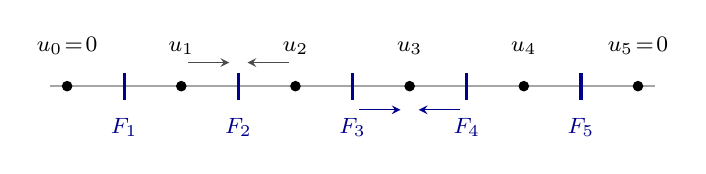
\begin{tikzpicture}[x=1.45cm, y=1cm, >=stealth]
        % the line, the nodes and the edges
        \draw[gray!70, thick] (-0.15,0) -- (5.15,0);
        \foreach \i in {0,1,2,3,4,5}
            \filldraw[black] (\i,0) circle (1.7pt);
        \foreach \i/\lab in {0/{u_0\!=\!0}, 1/{u_1}, 2/{u_2}, 3/{u_3}, 4/{u_4}, 5/{u_5\!=\!0}}
            \node[above=8pt, font=\footnotesize] at (\i,0) {$\lab$};
        \foreach \i in {0.5,1.5,2.5,3.5,4.5}
            \draw[blue!55!black, very thick] (\i,-0.17) -- (\i,0.17);
        \foreach \i/\lab in {0.5/{F_1}, 1.5/{F_2}, 2.5/{F_3}, 3.5/{F_4}, 4.5/{F_5}}
            \node[below=8pt, font=\footnotesize, blue!55!black] at (\i,0) {$\lab$};
        % G: two nodes -> the edge between them
        \draw[->, gray!60!black] (1.06,0.30) -- (1.42,0.30);
        \draw[->, gray!60!black] (1.94,0.30) -- (1.58,0.30);
        % -G^T: two edges -> the node between them
        \draw[->, blue!55!black] (2.56,-0.30) -- (2.92,-0.30);
        \draw[->, blue!55!black] (3.44,-0.30) -- (3.08,-0.30);
    \end{tikzpicture}
    \\[4pt]
    {\footnotesize
    $\displaystyle (G_1u)_2=\frac{u_2-u_1}{h}$ \quad(nodes $\to$ edges)
    \hspace{0.9cm}
    $\displaystyle (-G_1^\T\bs F)_3=\frac{F_4-F_3}{h}$ \quad(edges $\to$ nodes)}
    \caption{\footnotesize The staggered grid in one dimension, $N=4$. The state $u$ lives on the nodes ($\bullet$), the flux $F$ on the $N+1=5$ edges ($|$) between them; the two end edges are legitimate because the Dirichlet ghosts $u_0=u_5=0$ are known. The forward difference $G_1$ carries node values to the edges, and its negative transpose carries edge values back to the nodes as a divergence. Summing that divergence over all nodes telescopes, $\sum_i h\,(-G_1^\T\bs F)_i = F_{N+1}-F_1$, so whatever leaves one cell enters its neighbour exactly, at any $h$: the discretisation conserves mass identically rather than to $O(h^2)$.}
    \label{fig:staggered-grid}
\end{figure}

\paragraph{The operators as matrices.} Written out at $N=4$, the collocated first and second differences are the square matrices
\begin{equation}
    \label{eq:D1-L1-matrices}
    D_1 = \frac{1}{2h}\!\begin{pmatrix} 0&1&&\\ -1&0&1&\\ &-1&0&1\\ &&-1&0 \end{pmatrix}\!,
    \qquad
    L_1 = \frac{1}{h^2}\!\begin{pmatrix} -2&1&&\\ 1&-2&1&\\ &1&-2&1\\ &&1&-2 \end{pmatrix}\!,
\end{equation}
entries whose index falls outside $\{1,\dots,N\}$ being dropped --- that is exactly what the Dirichlet condition does, since those entries would multiply a ghost value of zero. Note that $D_1^\T = -D_1$: the collocated first difference is antisymmetric, as $\partial_x$ is. The staggered forward difference, by contrast, is \emph{rectangular},
\begin{equation}
    \label{eq:fwd-diff}
    (G_1 u)_m = \frac{u_m - u_{m-1}}{h},\quad m=1,\dots,N+1,
    \qquad
    G_1 = \frac{1}{h}\!\begin{pmatrix} 1&&&\\ -1&1&&\\ &-1&1&\\ &&-1&1\\ &&&-1 \end{pmatrix}\!,
\end{equation}
an $(N{+}1)\times N$ matrix,
because it produces one number per edge and there are more edges than nodes. That extra row is not a bookkeeping detail: it is the flux through the last edge, and a square operator has nowhere to put it. Its negative transpose,
\begin{equation}
    \label{eq:discrete-div}
    (-G_1^\T\bs F)_i = \frac{F_{i+1}-F_i}{h},
\end{equation}
is the discrete divergence, subtracting the flux entering node $i$ from the left from the flux leaving it on the right.

\paragraph{Which pairs are consistent.} In the continuum the second derivative is the first applied twice, and for the Laplacian this has a sharper form: integrating by parts, $\int u\,\nabla^2u = -\int|\nabla u|^2$, so $\nabla^2$ is minus the gradient composed with its own adjoint. It is worth asking which of the discrete operators inherits that. For the staggered pair the answer is exact,
\begin{equation}
    \label{eq:G-lap-identity}
    \boxed{\;-\,G_1^\T G_1 = L_1,
    \qquad\text{hence}\qquad
    -\bigl(G_x^\T G_x + G_y^\T G_y\bigr) = L_x + L_y = L, \;}
\end{equation}
with the 2D operators defined in \eqref{kron-derivatives} below. This is an identity, not an approximation, and it holds in the boundary rows too --- the $(N{+}1)$-th row of $G_1$ contributes precisely the stencil entry that an $N\times N$ collocated backward difference would drop, which is why the edge space cannot be dispensed with. The solver asserts \eqref{eq:G-lap-identity} on the assembled matrices at run time and aborts if it fails.

For the collocated pair it fails. Since $D_1$ is antisymmetric, $-D_1^\T D_1 = D_1^2$, and squaring the central difference gives
\begin{equation}
    \label{eq:wide-laplacian}
    (D_1^2u)_i = \frac{u_{i+2}-2u_i+u_{i-2}}{4h^2}
    \;\neq\;
    \frac{u_{i+1}-2u_i+u_{i-1}}{h^2} = (L_1u)_i .
\end{equation}
Both sides are perfectly good second-order approximations of $\partial_x^2u$; they simply are not the same matrix. The left one is the second difference on a grid of spacing $2h$: it never touches the nearest neighbours $u_{i\pm1}$ at all, so it couples only nodes of the same parity and leaves the odd and even sublattices of the grid completely independent of each other. The compact $L_1$ does not.

This is the whole of the difficulty, and it can be stated as a rule: \emph{wherever an operator enters the calculation twice --- once as the drift and once, squared, in the noise --- both copies must be built from the same difference operator}. If they are not, the two do not cancel, and \cref{sec-stencil-choice} works out how large the resulting error is. It does not vanish as $h\to0$.

\paragraph{Two dimensions.} Flatten the grid column-wise, $k(i,j) = i + (j-1)N$, so that $u\in\R^{N^2}$. Every 2D operator is then a Kronecker product of a 1D operator with an identity, one factor per axis:
\begin{align}
    \label{kron-derivatives}
    D_x = \eye_N \otimes D_1, & \quad D_y = D_1 \otimes \eye_N
    \\
    L_x = \eye_N \otimes L_1, & \quad L_y = L_1 \otimes \eye_N
    \\
    D_{xy} = D_1 \otimes D_1, & \quad L = L_x + L_y
    \\
    \label{kron-G}
    G_x = \eye_N \otimes G_1, & \quad G_y = G_1 \otimes \eye_N
\end{align}
The collocated ones are sparse $N^2\times N^2$ matrices; $G_x$ maps the $N^2$ nodes to the $N(N{+}1)$ $x$-edges and $G_y$ to the $N(N{+}1)$ $y$-edges. For completeness, the collocated stencils these encode are
\begin{align}
    (\partial_x u)_{i,j} &= \frac{u_{i+1,j} - u_{i-1,j}}{2h},
    &
    (\partial_y u)_{i,j} &= \frac{u_{i,j+1} - u_{i,j-1}}{2h}
    \\
    (\partial_x^2 u)_{i,j} &= \frac{u_{i+1,j} - 2u_{i,j} + u_{i-1,j}}{h^2},
    &
    (\partial_y^2 u)_{i,j} &= \frac{u_{i,j+1} - 2u_{i,j} + u_{i,j-1}}{h^2}
    \\
    (\partial_x \partial_y u)_{i,j} &= \frac{u_{i+1,j+1} - u_{i-1,j+1} - u_{i+1,j-1} + u_{i-1,j-1}}{4h^2}\hspace{-3cm}
\end{align}
all of them second-order accurate in $h$.

\subsubsection{Assembly of the operator and noise}
For the $m$-component field, order the state $\bs\Psi\in\R^{mN^2}$ by stacking one whole grid per component --- all $N^2$ values of component $1$, then all $N^2$ of component $2$, and so on,
\begin{align}
    \label{state-ordering}
    \bs\Psi = \begin{pmatrix} \bs\psi^{(1)} \\ \bs\psi^{(2)} \\ \vdots \\ \bs\psi^{(m)} \end{pmatrix},
    \qquad
    \bs\psi^{(a)}\in\R^{N^2},\ \ \bs\psi^{(a)}_{k(i,j)} = \psi^a(\r_{i,j})
\end{align}
so that the entry at position $(a-1)N^2+k$ is component $a$ at grid point $k$: the grid index runs through its whole range before the component index advances, just as $i$ does before $j$ in $k(i,j)$. This is what puts the $m\times m$ factor on the left of every Kronecker product below; the opposite convention, keeping the $m$ components of a single grid point adjacent, would serve as well but would transpose every $\otimes$.

A generic $\A(\r)$ decomposes as a sum of terms $\bs c(\r)\cdot \partial^\alpha$ with $\bs c(\r)$ an $m\times m$ matrix-valued coefficient and $\partial^\alpha \in\{\eye, \partial_x, \partial_y, \partial_x^2, \partial_y^2, \partial_x\partial_y\}$. In the ordering \eqref{state-ordering}, each such term discretizes as an $m\times m$ block matrix,
\begin{align}
    \label{term-assembly}
    \tilde{\A}_{\text{term}} = \sum_{a,b=1}^m E_{ab}\otimes \Big(\mathrm{diag}\big[c^{ab}(\r_k)\big]_{k=1}^{N^2}\cdot \bs D^\alpha\Big)
\end{align}
where $E_{ab}$ is the $m\times m$ matrix unit with a $1$ in position $(a,b)$, and $\bs D^\alpha \in \{\eye,D_x,D_y,L_x,L_y,D_{xy}\}$. Summing over all terms gives $\tilde{\A}\in\R^{mN^2\times mN^2}$. Since $\delta(\r-\r')$ is regularized on the grid as $\delta_{kk'}/h^2$, the discrete noise covariance is
\begin{align}
    \label{Q-matrix}
    \bs Q = \frac{1}{h^2}\left(\tilde{\B} + \tilde{\B}^\T\right)
\end{align}
(the symmetrization ensures $\bs Q = \bs Q^\T$).

\paragraph{The noise is not discretized like the drift.} It is tempting to build $\tilde\B$ with the same $\bs D^\alpha$ as $\tilde\A$, but that is wrong, and \cref{sec-stencil-choice} shows how wrong. Our noises are in divergence form: $f^a = \partial_i F^a_i$ with a local flux covariance
\begin{equation}
    \label{eq:flux-cov}
    \la F^a_i(\r)\,F^b_j(\r')\ra = M^{ab}_{ij}(\r)\,\delta(\r-\r').
\end{equation}
The one-dimensional case shows what to do, in three steps. The flux $\bs F$ lives on the edges, so its discrete covariance is $\la\bs F\bs F^\T\ra = \mathrm{diag}[M(\r_\text{edge})]/h$, the $1/h$ being the grid form of $\delta(x-x')$. The force on the state is its divergence, $\bs f = -G_1^\T\bs F$ by \eqref{eq:discrete-div}. Hence
\begin{equation}
    \label{eq:Q-1d}
    \bs Q \;=\; \la\bs f\bs f^\T\ra
    \;=\; G_1^\T\,\la\bs F\bs F^\T\ra\,G_1
    \;=\; \frac1h\,G_1^\T\,\mathrm{diag}\bigl[M(\r_\text{edge})\bigr]\,G_1 .
\end{equation}
Two features of \eqref{eq:Q-1d} are worth naming, because both survive into two dimensions and into \cref{sec-noise-cutoff}. First, it is a \emph{congruence}: a matrix of the form $S\,\mathrm{diag}(M)\,S^\T$ is automatically positive semi-definite whenever $M\ge0$ pointwise, so condition (ii) of \cref{sec-lyap-conditions} needs no separate check. Second, when $M$ is constant it collapses by \eqref{eq:G-lap-identity} to $\bs Q = -(M/h)\,L_1$ --- \emph{the noise matrix is the drift matrix}, up to a constant. That is what a consistent pairing means in the most concrete possible terms, and it is exactly what the mismatched choice destroys.

In two dimensions the same construction, with the $i=j$ flux components living on the $i$-edges, gives
\begin{multline}
    \label{eq:Q-assembly}
    \bs Q = \frac{1}{h^2}\sum_{a,b} E_{ab}\otimes\Bigl[
      G_x^\T\,\mathrm{diag}\bigl[M^{ab}_{xx}(\r_{x\text{-edge}})\bigr]\,G_x
    + G_y^\T\,\mathrm{diag}\bigl[M^{ab}_{yy}(\r_{y\text{-edge}})\bigr]\,G_y \\
    {}+ D_x\,\mathrm{diag}\bigl[M^{ab}_{xy}(\r_k)\bigr]\,D_y^\T
    + D_y\,\mathrm{diag}\bigl[M^{ab}_{yx}(\r_k)\bigr]\,D_x^\T\Bigr]
    \;+\;\frac{1}{h^2}\sum_{a,b}E_{ab}\otimes\mathrm{diag}\bigl[\Lambda^{ab}(\r_k)\bigr],
\end{multline}
the last sum being any noise that is \emph{not} in divergence form (for us the rotational $\Lambda$ terms), which stays local at the nodes.

The mixed $i\neq j$ terms, by contrast, keep the collocated $D_x, D_y$ with node-sampled coefficients, and this too is forced rather than convenient. The reason is that they are a different \emph{shape} of object. The diagonal terms enter \eqref{eq:Q-assembly} as $G_i^\T\,\mathrm{diag}(M_{ii})\,G_i$ --- a square, the same operator on both sides --- which is precisely the situation in which the identity \eqref{eq:G-lap-identity} can apply and must be respected. The mixed term $M_{xy}$ carries two \emph{different} derivatives, one in $x$ and one in $y$; it forms no square, and there is no identity for it to satisfy. What it must preserve instead is a symmetry. Both derivatives at the same node give the symbol $\ii\sin\phi/h$, purely imaginary, so the mixed contribution goes as $\sin p\sin q$, which is odd in $p$; that oddness is what makes the angular average of $\hat k_i\hat k_jQ^\ss_{ij}$ vanish for a traceless $\Q^\ss$, as it must. Staggering the two derivatives would place them half a cell apart and attach a factor $\cos\bigl(\tfrac{q-p}{2}\bigr)$, destroying the parity and leaving a spurious $\Q^\ss$-proportional pedestal of relative size $\simeq0.09|\Q^\ss|$ that does not go away with refinement. The rule is therefore: \emph{each index pair uses the operator matching where its covariance lives} --- squared terms are phase-free and belong on the edges, mixed terms need both derivatives at the same point.

\paragraph{Drift terms in divergence form.} The same logic applies to any \emph{dissipative} drift term written as a divergence. For $\nabla\cdot(c(\r)\nabla\,\cdot\,)$ the consistent discretisation is
\begin{equation}
    \label{eq:drift-divform}
    \nabla\cdot\bigl(c\,\nabla\,\cdot\,\bigr) \;\longrightarrow\;
    -\sum_i G_i^\T\,\mathrm{diag}\bigl[c(\r_{i\text{-edge}})\bigr]\,G_i ,
\end{equation}
that is: take the gradient onto the edges, multiply by the coefficient sampled \emph{there}, and take the divergence back. In one dimension it reads
\begin{equation}
    \label{eq:divform-1d}
    \bigl[\partial_x(c\,\partial_xu)\bigr]_i \;\longrightarrow\;
    \frac{c_{i+1/2}\,(u_{i+1}-u_i) \;-\; c_{i-1/2}\,(u_i-u_{i-1})}{h^2},
\end{equation}
in which the coupling between nodes $i$ and $i+1$ is $c_{i+1/2}/h^2$ read from either end: the matrix equals its own transpose, exactly, as the continuum operator does. Expanding by the product rule at the nodes instead, $c\,L + (\partial_xc)D_x + (\partial_yc)D_y$, is also second-order but is \emph{not} self-adjoint --- the coupling from $i$ to $i+1$ then carries $c_i+\tfrac12h\,\partial_xc|_i$ while the reverse coupling carries $c_{i+1}-\tfrac12h\,\partial_xc|_{i+1}$, and the two agree only up to $O(h^2)$. For the defect steady state of \cref{sec-noiseless-dynamics} the resulting asymmetry is $1.6\times10^{-2}$ and the two operators differ by $2.8\%$ at $N=41$. Note that with $c\equiv1$ \eqref{eq:drift-divform} reduces to $L$, so the plain Laplacian needs no change; and by \eqref{eq:G-lap-identity} neither does $L_x - L_y = -G_x^\T G_x + G_y^\T G_y$, which is already the exact staggered double divergence of a traceless $\Q$. The mixed derivative $D_{xy}$ is likewise \emph{already} the exact staggered composite $\mathrm{div}_x\bigl(\partial_y Q_{xy}|_\mathrm{corner}\bigr) + \mathrm{div}_y\bigl(\partial_x Q_{yx}|_\mathrm{corner}\bigr)$ with $Q_{xy}$ averaged from the nodes to the cell corners, so its zero at the Nyquist wavevector is intrinsic to $\partial_x\partial_y$ on a grid and not a defect of the stencil.

\subsubsection{Discrete Lyapunov equation and conditions}
\label{sec-lyap-conditions}
The discretized steady-state covariance $\mathbf{C} = \la \bs\Psi \bs\Psi^\T\ra_{ss}\in\R^{mN^2\times mN^2}$ satisfies
\begin{align}
    \label{lyapunov-discrete}
    \tilde{\A}\mathbf{C} + \mathbf{C}\tilde{\A}^\T = -\bs Q
\end{align}
A unique solution exists and is symmetric positive semi-definite provided:
\begin{align}
    &\text{(i) } \mathrm{Re}\,\lambda_k(\tilde{\A}) < 0 \text{ for all } k
    &&\text{(stability of the linearization)}
    \\
    &\text{(ii) } \bs Q \succeq 0
    &&\text{(covariance positivity)}
\end{align}
Condition (i) is the requirement that $\psi=0$ is a linearly stable state; if it fails, the assumption of steady-state Gaussian fluctuations breaks down. Condition (ii) is automatic when $\B(\r)$ is a bona fide covariance kernel; if the discretization introduces a small negative spectrum through mixed derivatives, project $\bs Q$ onto its positive part. A stronger but easier-to-verify sufficient condition for (i) is that $(\tilde{\A}+\tilde{\A}^\T)/2$ is negative definite.

In the ordering \eqref{state-ordering}, $\mathbf{C}$ has an $m\times m$ block structure with blocks $\mathbf{C}^{ab}\in\R^{N^2\times N^2}$, and the single-point variance is
\begin{align}
    \label{variance-extraction}
    \Sigma^{ab}(\r_{i,j}) = \mathbf{C}^{ab}_{k(i,j),\,k(i,j)}
\end{align}
Note that $\Sigma\sim h^{-2}$ as $h\to 0$: with delta-correlated noise the continuum single-point variance diverges, and the grid is what regulates it. The physically meaningful output is obtained by giving the noise the finite correlation length it physically has, as \cref{sec-noise-cutoff} does; equivalently one may smooth the covariance, $\int W(\r-\r')\mathbf{C}(\r',\r'')W(\r-\r'')\d\r'\d\r''$, the two being the same calculation by \eqref{eq:W-commutes}.

\subsubsection{Pseudocode}
\begin{verbatim}
Input:  N, h, coefficient fields for A(r) and B(r), m
Output: variance Sigma^{ab}(r_{i,j})

1.  Build 1D matrices D1, L1 of size N x N (Dirichlet, entries outside dropped)
    and the forward difference G1 of size (N+1) x N.
2.  Assemble 2D operators via Kronecker products:
        Dx = kron(I_N, D1),   Dy  = kron(D1, I_N)
        Lx = kron(I_N, L1),   Ly  = kron(L1, I_N),   Dxy = kron(D1, D1)
        Gx = kron(I_N, G1),   Gy  = kron(G1, I_N)
    Assert -(Gx^T Gx + Gy^T Gy) == Lx + Ly exactly; else abort.
3.  Assemble A_tilde in R^{mN^2 x mN^2}:
      A_tilde = 0
      for each term  c(r) . d^alpha  in A(r), for a, b in 1..m:
        if the term is a divergence  div(c grad .):
          A_tilde -= kron(E_ab, Gx^T @ diag(c^ab|xe) @ Gx
                              + Gy^T @ diag(c^ab|ye) @ Gy)
        else:
          A_tilde += kron(E_ab, diag(c^ab(r_k)) @ D^alpha)
4.  Assemble Q from the flux covariance M^ab_ij, NOT like A_tilde:
      Q = 0
      for a, b in 1..m:
        Q += kron(E_ab, Gx^T @ diag(M^ab_xx|xe) @ Gx
                      + Gy^T @ diag(M^ab_yy|ye) @ Gy
                      + Dx @ diag(M^ab_xy(r_k)) @ Dy^T
                      + Dy @ diag(M^ab_yx(r_k)) @ Dx^T
                      + diag(local non-divergence noise)) / h^2
      Q = (Q + Q^T) / 2.
5.  Check: max Re spec(A_tilde) < 0; else abort (linearization unstable).
    Check: min eig Q >= 0 (Arnoldi on the sparse matrix).
6.  Solve continuous Lyapunov equation
        A_tilde @ C + C @ A_tilde^T = -Q
    e.g. scipy.linalg.solve_continuous_lyapunov(A_tilde, -Q).
7.  Partition C into m x m blocks of size N^2 x N^2; extract diagonal
    entries of each block:
        Sigma^{ab}(r_{i,j}) = C[(a-1)*N^2 + k(i,j), (b-1)*N^2 + k(i,j)].
\end{verbatim}
Cost is dominated by the Lyapunov solve, $\mathcal{O}((mN^2)^3)$ with the Bartels--Stewart algorithm. On a laptop this is comfortable for $mN^2 \lesssim 10^4$, i.e.\ $N\lesssim 50$ for $m$ small; for larger grids, use sparse Krylov methods (e.g.\ rational Krylov, ADI) that exploit the sparsity of $\tilde{\A}$.

\subsection{Why the choice of difference operators matters}
\label{sec-stencil-choice}

Every operator in \eqref{kron-derivatives} is second-order accurate, so one might expect the choice among them to be a matter of taste, correctable by refining $h$. For the equal-point variance it is not. This subsection prices the mismatch \eqref{eq:wide-laplacian}: in one dimension, where the whole calculation can be done on paper, pairing a divergence-form noise with the wrong stencil costs a factor of exactly two; in the two-dimensional problem the solver actually runs it costs a factor $2.752$. Neither shrinks as $h\to0$.

\paragraph{The smallest problem that shows it.} Take a single field on a line, diffusing and driven by a conserved noise --- \eqref{eq:sde} stripped to its essentials:
\begin{equation}
    \label{eq:toy-1d}
    \partial_tu = \gamma_0\partial_x^2u + \partial_xF,
    \qquad
    \la F(x,t)F(x',t')\ra = \kappa\,\delta(x-x')\,\delta(t-t').
\end{equation}
In the continuum the force on $u$ is $f = \partial_xF$, so its spectral density carries a factor $k^2$; the relaxation rate is $\gamma_0k^2$; and the steady spectrum, being the ratio of the two, is $\kappa/2\gamma_0$ at every $k$ --- the exact cancellation of \cref{sec-rho-only}, in its simplest setting.

On the grid the same balance holds mode by mode. A plane wave $\ee^{\ii\phi n}$ diagonalises every constant-coefficient difference operator, so \eqref{lyapunov-discrete} decouples into $2|\hat A|\hat C = \hat Q$ and the variance of a single mode is a \emph{ratio},
\begin{equation}
    \label{eq:mode-balance}
    \hat C(\phi) \;=\; \frac{\hat Q(\phi)}{2\,|\hat A(\phi)|}.
\end{equation}
The drift contributes the denominator, $\hat A = \gamma_0\hat L_1$ with $\hat L_1 = (\ee^{\ii\phi}-2+\ee^{-\ii\phi})/h^2 = -4\sin^2(\phi/2)/h^2$. The numerator depends on which difference the noise was built from, and this is where the two choices part company:
\begin{itemize}
    \item \emph{staggered.} With $\bs Q = (\kappa/h)\,G_1^\T G_1$ from \eqref{eq:Q-1d}, the symbol is $|\hat G_1|^2 = |\ee^{\ii\phi}-1|^2/h^2 = 4\sin^2(\phi/2)/h^2$, which is $-\hat L_1$ \emph{identically} --- that is \eqref{eq:G-lap-identity} read in Fourier space. Numerator and denominator cancel and
    \begin{equation}
        \label{eq:Chat-1d-good}
        \hat C(\phi) \;=\; \frac{\kappa}{2\gamma_0 h}\qquad\text{for every mode,}
    \end{equation}
    flat, exactly as in the continuum.
    \item \emph{collocated.} With $\bs Q = (\kappa/h)\,D_1D_1^\T$ the symbol is $|\hat D_1|^2 = \sin^2\phi/h^2$ instead, and since $\sin^2\phi = 4\sin^2\frac\phi2\cos^2\frac\phi2$,
    \begin{equation}
        \label{eq:Chat-1d-bad}
        \hat C(\phi) \;=\; \frac{\kappa}{2\gamma_0 h}\;\cos^2\frac{\phi}{2}.
    \end{equation}
\end{itemize}
The equal-point variance is the average of $\hat C$ over the band, $\Sigma = \la\hat C\ra_\phi$, because the modes are complete at every node. So the two schemes differ by
\begin{equation}
    \label{eq:half-1d}
    \boxed{\;\frac{\Sigma_\text{collocated}}{\Sigma_\text{staggered}}
    \;=\; \la\cos^2\tfrac{\phi}{2}\ra_{[-\pi,\pi]}
    \;=\; \frac12 \;}
\end{equation}
--- exactly one half, at every $h$, for a scheme that is second-order accurate and passes every classical consistency check.

\paragraph{Why refining the grid does not help.} The failure is sharpest on the shortest mode the grid can carry, the sawtooth $u_n=(-1)^n$. The central difference annihilates it \emph{exactly}, $(D_1u)_n = [(-1)^{n+1}-(-1)^{n-1}]/2h = 0$: it skips the centre point, and the two neighbours it does see are equal, so it reports no variation at all. The compact Laplacian meanwhile damps that mode as hard as it can, $(L_1u)_n = -4(-1)^n/h^2$. Grid-scale modes are therefore dissipated without being driven, and they starve --- this is $\cos^2(\phi/2)\to0$ at $\phi=\pi$ in \eqref{eq:Chat-1d-bad}.

Refining $h$ cannot repair it, because the equal-point variance is dominated by exactly those modes: the spectrum \eqref{eq:Chat-1d-good} is flat, so every mode contributes equally, and halving $h$ simply adds another octave of short modes that are treated just as badly. Second-order accuracy constrains only the $\phi\to0$ end of the band (\cref{fig:stencil-R}a), which is the part that contributes least. The damage is a fixed fraction of the answer, not an error that converges away.

\paragraph{The same calculation in two dimensions.} Nothing changes but the bookkeeping. \Cref{fig:stencil-R} shows the two pictures; the rest of this subsection is the two-dimensional version of \eqref{eq:half-1d}, and gives $2.752$ in place of $2$.

\begin{figure}[h!]
    \centering
    \includegraphics[width=0.98\textwidth]{media/stencil_R_weight.pdf}
    \caption{\footnotesize \textbf{(a)} The two one-dimensional symbols the solver pairs against each other: the drift's $-h^2\hat L_1 = 4\sin^2(\phi/2)$ and the noise's $h^2|\hat D_1|^2 = \sin^2\phi$. They agree as $\phi\to0$ --- all that second-order accuracy guarantees --- and diverge completely by the Nyquist wavevector $\phi=\pi$, where the central difference returns to zero while the Laplacian damps maximally. \textbf{(b)} The resulting weight $R(p,q)$ of \eqref{eq:Ck-lattice} on the Brillouin zone: $1$ at the origin, $1/2$ at $(\pi/2,\pi/2)$, $0$ at the corner. The spectrum being otherwise flat, the pedestal is the zone average $\la R\ra$.}
    \label{fig:stencil-R}
\end{figure}

In the bulk a plane wave $\ee^{\ii(pi+qj)}$ diagonalises the constant-coefficient operators, and \eqref{eq:mode-balance} holds with $\phi$ replaced by the pair $(p,q)$. Take the density sector of \cref{sec-rho-only}: drift $\gamma_0 L$ with $L$ the compact Laplacian, noise $\bs Q = (\kappa/h^2)(D_xD_x^\T + D_yD_y^\T)$ with $D$ the central difference. Their symbols are $|\hat D_1|^2 = \sin^2\phi/h^2$ against $-\hat L_1 = 4\sin^2(\phi/2)/h^2$, which are not equal (\cref{fig:stencil-R}a), so \eqref{eq:mode-balance} with $\kappa/(2\gamma_0)=\zeta/(B\rho_0)$ gives
\begin{equation}
    \label{eq:Ck-lattice}
    \hat C(p,q) \;=\; \frac{\zeta}{B\rho_0h^2}\,R(p,q),
    \qquad
    R \;=\; \frac{\sin^2p+\sin^2q}{4\bigl(\sin^2\frac p2+\sin^2\frac q2\bigr)} .
\end{equation}
Equivalently $R = \bigl(\sin^2\tfrac p2\cos^2\tfrac p2 + \sin^2\tfrac q2\cos^2\tfrac q2\bigr) / \bigl(\sin^2\tfrac p2 + \sin^2\tfrac q2\bigr)$, a $\sin^2$-weighted average of $\cos^2(p/2)$ and $\cos^2(q/2)$: it is $1$ at $\k=0$, $1/2$ at $(\pi/2,\pi/2)$, and $0$ at the zone corner. Along an axis it reduces to the one-dimensional $R(p,0) = \cos^2(p/2)$ of \eqref{eq:Chat-1d-bad}, as it must.

The argument then runs exactly as in one dimension, except that the average is now over an area, and most of the Brillouin zone's area lies at large $|\k|$ --- precisely where the two stencils disagree (\cref{fig:stencil-R}b). The damage is again $h$-independent, and equal to the zone average
\begin{equation}
    \label{eq:R-average}
    \la R\ra \;=\; \frac{1}{\pi^2}\int_0^\pi\!\!\int_0^\pi R(p,q)\,\d p\,\d q
    \;=\; 0.363380 ,
\end{equation}
and classical consistency ($R\to1$ as $\k\to0$) is simply the wrong criterion for this observable.

\paragraph{The remedy.} Build the divergence-form noise from $G_i$, whose Gram matrix \emph{is} the drift Laplacian by \eqref{eq:G-lap-identity}. Numerator and denominator of \eqref{eq:mode-balance} then carry the identical symbol $4(\sin^2\frac p2+\sin^2\frac q2)/h^2$, so $R\equiv1$ for every mode and
\begin{equation}
    \label{eq:pedestal-R1}
    \boxed{\;\Sigma^{\rho\rho}(\r) \;=\; \frac{\zeta\,\rho_\ss(\r)}{B\rho_0\,h^2}
    \;=\;\frac{\zeta\rho_\ss(\r)}{B\rho_0}\int_\mathrm{BZ}\!\frac{\d^2\k}{(2\pi)^2},\;}
\end{equation}
the second form because $\hat C$ is now mode-independent and $\int_\mathrm{BZ}\d^2\k/(2\pi)^2 = (2\pi/h)^2/(2\pi)^2 = h^{-2}$ exactly: a grid of spacing $h$ is a \emph{square} Brillouin-zone cutoff, and with a consistent stencil its measure is all that survives --- no fitted constant. Two further checks come free:
\begin{itemize}
    \item because $\hat C$ no longer depends on the mode, completeness $\sum_k|v_k(\r)|^2=1$ makes $\bs\Sigma$ uniform at every node, \emph{including} those adjacent to the boundary. The isotropic Dirichlet boundary layer in the variance was therefore an artifact --- though not of the stencil pairing alone, since a collocated noise cannot carry flux through $\partial\Omega$ either, and it is that second and silent choice which produced the rim. \Cref{sec-bc} separates the two, and shows that the uniformity is a continuum consequence of drift and noise sharing a mobility rather than a fact about lattice modes;
    \item the $\Q^\ss$-dependent part of the pedestal must vanish by the angular cancellation of the traceless $\Q^\ss$, which is what fixes the treatment of the mixed flux terms described after \eqref{eq:Q-assembly}.
\end{itemize}

\paragraph{Measured.} Solving \eqref{lyapunov-discrete} for the density sector at $\rho_\ss=1$, $\Q^\ss=0$, changing only the noise assembly and holding $\tilde\A$ fixed (legitimate by \eqref{eq:G-lap-identity}):

\begin{center}
\footnotesize
\begin{tabular}{lccc}
\hline
 & \multicolumn{2}{c}{central difference} & $G$-based \\
$N$ & $\Sigma h^2B\rho_0/\zeta$ & dev.\ from $\la R\ra$ & $\Sigma h^2B\rho_0/\zeta$ \\
\hline
$41$ & $0.3633125$ & $-0.019\%$ & $1.00000000$ \\
$61$ & $0.3633590$ & $-0.006\%$ & $1.00000000$ \\
$81$ & $0.3633710$ & $-0.003\%$ & $1.00000000$ \\
\hline
\end{tabular}
\end{center}

\noindent Reading across:
\begin{itemize}
    \item the central difference converges to \eqref{eq:R-average}, confirming that the deficit is the zone average and not a discretisation error that refinement would remove;
    \item the $G$-based noise reproduces \eqref{eq:pedestal-R1} to all printed digits and uniformly over the whole grid --- relative spread at round-off, against $0.60$ for the central-difference variant, whose first interior node sits at $0.66$ of the bulk value --- a suppression \cref{sec-bc} attributes to the blocked boundary flux rather than to the Dirichlet condition;
    \item in the full three-field problem the same change moves the bulk coefficient from $0.362$ to $0.997$ at $N=41$, a factor $2.744$ against the predicted $2.752$, the residual $0.3\%$ being the $\delta\Q$ coupling, which is $O(1/B)$ and unrelated to the stencils;
    \item stability and positivity are unaffected: $\max\mathrm{Re}\,\lambda = -0.0968$ either way, and $\bs Q$ stays positive definite.
\end{itemize}

Only \emph{dissipative} operators and their noise partners are constrained this way, because only they appear on both sides of \eqref{eq:mode-balance}. Reactive couplings have no noise partner and are governed by accuracy alone --- which is why $D_{xy}$ needs no change even though $\hat D_{xy} = -\sin p\sin q/h^2$ also vanishes at the zone corner.


\subsection{Boundary conditions}
\label{sec-bc}

The Dirichlet condition was imposed once, below \eqref{ou-noise}, and not revisited. It deserves to be, on two counts: it is not one condition but three, and the equal-point variance reports it in a way that is easy to read backwards.

\paragraph{Three conditions, not one.} Posing \eqref{ou-model} on a bounded domain requires
\begin{equation}
    \label{eq:bc-triple}
    \text{(a)}\quad \rho_\ss,\Q^\ss\big|_{\partial\Omega},
    \qquad
    \text{(b)}\quad \psi\big|_{\partial\Omega},
    \qquad
    \text{(c)}\quad \bs F\cdot\nh\big|_{\partial\Omega},
\end{equation}
the steady state the fluctuations live on, the fluctuating field itself, and the noise flux of \eqref{eq:flux-cov}. The third is the one that goes unnoticed. In the continuum it constrains $\bs F$ on a set of measure zero and looks as though it could not matter; on the grid it is an explicit choice, and \cref{fig:staggered-grid} has already drawn it. The flux lives on the $N+1$ edges, two of which straddle $\partial\Omega$. Keeping them lets the noise carry material across the boundary; dropping them replaces $G_1$ by an $(N{-}1)\times N$ matrix $G_1^\circ$ whose Gram matrix is no longer \eqref{eq:G-lap-identity} but
\begin{equation}
    \label{eq:G-neumann}
    -G_1^{\circ\T}G_1^\circ = L_1^{\mathrm N},
    \qquad
    L_1^{\mathrm N} = \frac{1}{h^2}\!\begin{pmatrix} -1&1&&\\ 1&-2&1&\\ &1&-2&1\\ &&1&-1 \end{pmatrix}\!,
\end{equation}
the Neumann Laplacian --- $L_1$ with its two corner entries changed, which is exactly where a node that has lost a neighbour differs from one that has not. Condition (c) is therefore the choice of which Laplacian the \emph{noise} is built on, while (b) fixes the one the \emph{drift} is built on, and nothing in the assembly forces the two to agree.

One consequence is worth recording before going further. The collocated $D_1$ of \eqref{eq:D1-L1-matrices} has no edge space at all, hence no end rows to keep or drop, and a noise built from it cannot carry flux across $\partial\Omega$ under any circumstances. The scheme criticised in \cref{sec-stencil-choice} was thus making a second and silent choice on top of the stencil error --- it was blocking the flux --- and that, rather than the Dirichlet condition, is where the suppressed first interior node reported after \eqref{eq:pedestal-R1} comes from.

\begin{table}[h!]
\centering\footnotesize
\begin{tabular}{cccp{5.0cm}l}
\hline
$\rho_\ss$ & $\psi$ & $\bs F\cdot\nh$ & what the combination asserts & \\
\hline
D & D & free    & a window cut from a larger colony: the surroundings fix the mean and exchange particles across it & \textbf{consistent} \\
N & N & blocked & a container wall: nothing crosses it and the number inside is conserved & \textbf{consistent} \\
\hline
D & D & blocked & the mean is held from outside, but no particle may cross & (b),\,(c) \\
D & N & free    & particles cross freely, yet $\psi$ may not develop a gradient & (b),\,(c) \\
N & N & free    & sealed for the mean, leaky for the noise & (b),\,(c) \\
N & D & blocked & nothing crosses, yet $\psi$ is pinned at the wall & (a),\,(b),\,(c) \\
\hline
D & N & blocked & the mean is maintained from outside, the fluctuating number sealed in & (a),\,(b) \\
N & D & free    & a sealed box whose wall nonetheless pins $\psi$ & (a),\,(b) \\
\hline
\end{tabular}
\caption{\footnotesize The eight combinations of \eqref{eq:bc-triple}. D denotes a pinned (Dirichlet) condition and N a no-flux (Neumann) one. The last column names the pair of conditions that contradict each other. Only the first two rows are physically coherent; the solver runs the first.}
\label{tab:bc-eight}
\end{table}

\paragraph{Which combinations are consistent.} Conditions (b) and (c) are not independent statements. Both answer the same physical question --- whether a bacterium may cross $\partial\Omega$ --- once of the mean field and once of the fluctuation. Pinning $\psi$ at the wall says that whatever lies outside holds the density there fixed, and it can only do that by exchanging particles; particles that cross carry their shot noise with them, so $\bs F\cdot\nh$ cannot vanish. A wall that nothing crosses, conversely, pins nothing, and both the deterministic and the stochastic flux through it are zero. Condition (a) must then follow (b), since the steady state and the fluctuations see the same wall. Of the eight rows of \cref{tab:bc-eight} two survive:
\begin{itemize}
    \item \textbf{reservoir.} $\rho_\ss,\Q^\ss$ pinned, $\psi|_{\partial\Omega}=0$, flux free. The boundary is a window cut out of a larger colony, at whose edge the texture has already reached its far field. This is what the solver runs, and it is the condition under which $\partial\Omega$ carries no physical meaning of its own.
    \item \textbf{sealed.} $\nh\cdot\nabla\rho_\ss=0$, $\nh\cdot\nabla\psi=0$, flux blocked. The boundary is a container wall; nothing crosses it, and the total number inside is conserved exactly, fluctuation included.
\end{itemize}

\paragraph{Both consistent choices give a flat pedestal.} Suppose the drift and the noise can be written with a common mobility,
\begin{equation}
    \label{eq:fdt-split}
    \tilde\A = -MK,\qquad \bs Q = 2TM
    \qquad\Longrightarrow\qquad
    \mathbf{C} = T\,K^{-1},
\end{equation}
with $M=M^\T\succeq0$ and $K=K^\T\succ0$; substituting into \eqref{lyapunov-discrete} verifies it in one line. The content is in what has disappeared. $\mathbf{C}$ does not depend on $M$ --- and $M$ is precisely where the boundary condition lives, since choosing Dirichlet or Neumann \emph{is} choosing the domain of the Laplacian $M$ is built from. Whatever the wall does, it cannot reach the equal-time covariance through $M$.

The density sector is of this form. Its drift is $\gamma_0L$, and with a consistent stencil \eqref{eq:Q-1d} makes its noise $-(\kappa/h^2)L$ with $\kappa = 2\zeta/\xi_0\rho_0$, both built from the same $L$: take $M=\gamma_0(-L)$ and $K = k/\rho_\ss$, the local Hessian of an ideal-gas free energy. Only the ratio $T/k$ is then fixed, by the noise amplitude, and it is $\kappa/2\gamma_0 = \zeta/B\rho_0$, so
\begin{equation}
    \label{eq:C-local}
    \mathbf{C}(\r,\r') = \frac{\zeta\,\rho_\ss(\r)}{B\rho_0}\;\delta(\r-\r'),
\end{equation}
which on the grid, where $\delta(\r-\r')\to\delta_{kk'}/h^2$, is \eqref{eq:pedestal-R1} once more. Since $K$ is a multiplication operator so is $K^{-1}$, and $\mathbf{C}$ is therefore strictly local: the variance is the same multiple of $\rho_\ss$ at every point, the wall-adjacent ones included, and there are no correlations between distinct points through which the wall could make itself felt. This is a continuum statement; the completeness argument given after \eqref{eq:pedestal-R1} is its lattice shadow. A consistent stencil is nothing other than the discrete form of the split \eqref{eq:fdt-split}, which is why \eqref{eq:G-lap-identity} and \eqref{eq:fdt-split} stand or fall together.

Two disclaimers, pointing in opposite directions. The system is active and admits no free energy as a whole, and none is being claimed: \eqref{eq:fdt-split} asks only that drift and noise share a mobility, which is a structural property of the density block and says nothing about a temperature --- only the ratio $T/k$ ever appears. What is \emph{not} of this form are the couplings to $\delta\Q$, and they are exactly what makes \eqref{eq:C-local} approximate rather than exact, at relative order $\zeta/B$.

\paragraph{Where the boundary condition is visible instead.} Two places, and \eqref{eq:fdt-split} locates both.

A boundary layer in the variance requires a gradient term in the free energy. Give $K$ one, $K = 1/\chi - \kappa_{\rm el}\nabla^2$, and $K^{-1}$ becomes a Green's function of range $\sqrt{\kappa_{\rm el}\chi}$, which under a Dirichlet condition does vanish at the wall --- over that range, and not over $h$. The density sector has no such term. The $\delta\Q$ sector does: its drift carries $c_LL$ together with a mass term, so $\Var(\delta\Q)$ has a genuine boundary layer whose width is the nematic correlation length and which survives $h\to0$, while $\Var(\delta\rho)$ cannot have one at all. If the wall is what one wants to look at, $\delta\Q$ is where to look.

The difference between the two consistent choices is not a boundary layer either; it is the difference between the grand canonical and the canonical ensemble. Under the sealed condition $M$ is singular on the constant mode, the total is conserved, and \eqref{eq:fdt-split} holds on its complement,
\begin{equation}
    \label{eq:canonical}
    \mathbf{C} = T\left[K^{-1} - \frac{K^{-1}\mathbf{1}\,\mathbf{1}^\T K^{-1}}{\mathbf{1}^\T K^{-1}\mathbf{1}}\right],
\end{equation}
a rank-one subtraction of relative size $1/|\Omega|$ spread uniformly over the domain. It is finite, independent of $h$, and invisible at any single point: it shows up in the variance of a coarse-grained particle count, which is the observable that actually distinguishes an open box from a closed one.

\paragraph{What the inconsistent combinations do.} They break the split \eqref{eq:fdt-split} at the boundary --- the mobility that damps and the mobility that drives cease to agree there --- so $\mathbf{C} = TK^{-1}$ fails in the first cells while continuing to hold in the bulk. The sign of the failure follows from which of the two is missing. Damping across the wall without driving across it starves the adjacent cell and suppresses its variance, producing a rim; driving without damping does the reverse and produces a spike. A rim can therefore be had, but only by asserting that the wall is out of detailed balance, which is an assumption about what the wall is and not a consequence of pinning $\psi$.

\paragraph{The anisotropic residue at the wall.} \Cref{eq:C-local} used only the isotropic part of the flux covariance. For a traceless $\Q^\ss$ the conclusion is weaker, and what survives is worth having, because the wall is the only place in $\Sigma^{\rho\rho}$ where the anisotropy of the noise appears at all.

The mechanism is the one \cref{sec-stencil-choice} already set up, read at a different point of the domain. Each mode carries the flux covariance projected on its own wavevector,
\begin{equation}
    \label{eq:mode-projection}
    \hat C(\k) = \frac{\hat k_i\hat k_j M_{ij}}{2\gamma_0},
\end{equation}
and the variance at a point is the sum of $\hat C$ over modes weighted by $|v_{\k}(\r)|^2$. In the bulk that weight is flat in the direction of $\k$, the angular average of $\hat k_i\hat k_jM_{ij}$ is $\tfrac12\mathrm{tr}\,M$, and the traceless part cancels --- the same cancellation that fixes the mixed flux terms after \eqref{eq:Q-assembly}. Next to a Dirichlet wall it is not flat: $|v_p|^2\propto\sin^2(\alpha d)$, with $d$ the distance from the wall in units of $h$ and $\alpha$ the wavenumber normal to it, which is small for every mode whose normal wavelength exceeds $d$. What survives in the first few cells are the modes with $\hat\k$ along $\nh$, and those report $M_{nn}$ rather than its angular average. The difference is $M_{nn}-\tfrac12\mathrm{tr}\,M = Q^\ss_{nn}$, so
\begin{equation}
    \label{eq:wall-kernel}
    \frac{\Sigma^{\rho\rho}(d)}{\Sigma^{\rho\rho}_{\rm ped}} - 1
    \;=\; w_d\,\frac{Q^\ss_{nn}(\r)}{\rho_\ss(\r)},
    \qquad
    w_d = -\frac{1}{\pi^2}\!\int_0^\pi\!\!\!\int_0^\pi\!
    \cos(2\alpha d)\;
    \frac{\sin^2\frac\alpha2-\sin^2\frac\beta2}{\sin^2\frac\alpha2+\sin^2\frac\beta2}
    \,\d\alpha\,\d\beta ,
\end{equation}
a zone integral of the same kind as \eqref{eq:R-average}. Three of its properties can be read off without evaluating it. The $\cos(2\alpha d)$ is what is left of $2\sin^2(\alpha d) = 1-\cos(2\alpha d)$ after the $1$ has integrated to zero against a weight antisymmetric in $\alpha\leftrightarrow\beta$ --- so the residue is a boundary effect and nothing else, and $w_d\to0$ as $d\to\infty$ by Riemann--Lebesgue, recovering \eqref{eq:C-local} in the bulk. It depends on the integer $d$ alone and not on $h$, so refining the grid does not reduce it: it sits in the first few cells at a fixed fraction of a pedestal that is itself growing as $h^{-2}$. And its continuum counterpart $\int\!\d^2\k\,\cos(2k_nx)\,\hat k_i\hat k_jQ^\ss_{ij}/k^2$ diverges, so the amplitude is set by the regulator in exactly the way \eqref{eq:pedestal-R1} is. The pattern is meaningful; the size is not.

The pattern is fixed by the texture. With $\nh$ at angle $\alpha$ and the director at angle $\theta$,
\begin{equation}
    \label{eq:wall-angular}
    \frac{Q^\ss_{nn}}{\rho_\ss} = S\,\cos2(\alpha-\theta),
\end{equation}
so the variance is enhanced where the director runs into the wall, suppressed where it runs along it, and unshifted where it meets the wall at $45^\circ$ and the wall sees isotropic noise. For the $+1/2$ defect $\theta=\phi/2$ and \eqref{eq:wall-angular} becomes $S\cos(2\alpha-\phi)$: it is $+S\cos\phi$ on the walls normal to $\hat{\bs x}$ and $-S\cos\phi$ on those normal to $\hat{\bs y}$. The residue is therefore odd in $x$ --- low along one of the $x$-walls and high along the other, and changing sign midway along each of the other two (\cref{fig:bc-wall}). That it is an $m=1$ harmonic is a consequence of the charge being half-integer: $\theta=\phi/2$ is what turns $\cos2\theta$ into $\cos\phi$, where a $+1$ defect would give $\cos2\phi$ and a boundary pattern symmetric under $x\to-x$. It is the same harmonic, from the same source, as \eqref{eq:ddQ-m1}, and it therefore lands on the estimator \eqref{eq:A1-def} uses.

\begin{figure}[h!]
    \centering
    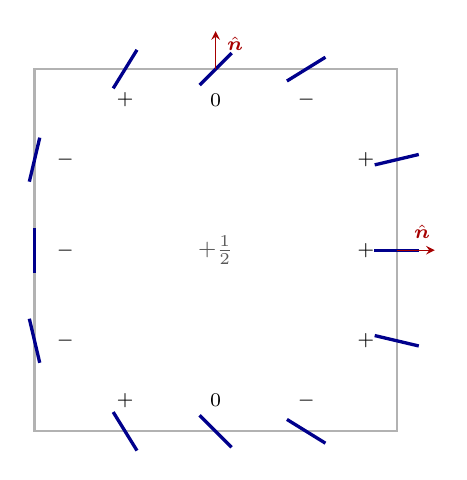
\begin{tikzpicture}[scale=1.15, >=stealth]
        \draw[gray!60, thick] (-2,-2) rectangle (2,2);
        \node[font=\footnotesize, gray!70!black] at (0,0) {$+\tfrac12$};
        \foreach \px/\py/\th/\ox/\oy/\sg in {%
            2/-1/-13.3/-0.34/0/+, 2/0/0/-0.34/0/+, 2/1/13.3/-0.34/0/+,
            -2/-1/-76.7/0.34/0/-, -2/0/90/0.34/0/-, -2/1/76.7/0.34/0/-,
            -1/2/58.3/0/-0.34/+, 0/2/45/0/-0.34/0, 1/2/31.7/0/-0.34/-,
            -1/-2/-58.3/0/0.34/+, 0/-2/-45/0/0.34/0, 1/-2/-31.7/0/0.34/-}
        {
            \draw[blue!55!black, very thick, rotate around={\th:(\px,\py)}]
                 ({\px-0.25},\py) -- ({\px+0.25},\py);
            \node[font=\scriptsize] at ({\px+\ox},{\py+\oy}) {$\sg$};
        }
        \draw[->, red!65!black] (2,0) -- (2.42,0);
        \node[font=\scriptsize, red!65!black, above] at (2.28,0.02) {$\nh$};
        \draw[->, red!65!black] (0,2) -- (0,2.42);
        \node[font=\scriptsize, red!65!black, right] at (0.02,2.28) {$\nh$};
    \end{tikzpicture}
    \caption{\footnotesize The wall residue \eqref{eq:wall-kernel} around $\partial\Omega$ for a $+1/2$ defect at the centre. Short bars are the director of the steady texture, $\theta=\phi/2$; signs are those of $Q^\ss_{nn}$, i.e.\ of $\cos(2\alpha-\phi)$ by \eqref{eq:wall-angular}. Where the director runs into the wall the surviving modes are the loud ones and the variance is raised; where it runs along the wall they are the quiet ones and it is lowered; where it meets the wall at $45^\circ$ the wall sees isotropic noise and the residue vanishes. The half-integer charge makes the winding half as fast as the azimuth, which is what leaves the pattern odd in $x$ rather than symmetric.}
    \label{fig:bc-wall}
\end{figure}

\paragraph{A consistency test away from the boundary.} \Cref{eq:Ck-lattice} supplies one for free. The isotropic part of the equal-time correlator is a delta function, \eqref{eq:autocorr-fourier}, and a delta in real space is a flat spectrum; the lattice spectrum is flat only if $R\equiv1$. So whenever $R\neq1$ its inverse transform has support at nonzero separation, and the mismatched stencil produces equal-time correlations between neighbouring nodes that the theory forbids. Since $R$ is a ratio of two symbols that agree only as $\k\to0$, this is a grid-scale correlation of order unity rather than a small effect --- which makes the isotropic part of the near-neighbour correlator a sharper diagnostic of the stencil pairing than the pedestal is, and one that needs no boundary at all.


\subsection{Noise with a finite correlation length}
\label{sec-noise-cutoff}

Even with a consistent stencil, \eqref{eq:pedestal-R1} is proportional to $h^{-2}$: a numerical parameter sets the answer, so the equal-point variance is not yet a prediction of anything. The divergence itself is not pathological --- it is shot noise, and $\la\delta N^2\ra/\la N\ra = \zeta/B$ independently of the cutoff --- but the regulator should be a property of the system, not of the mesh. And it already is one: the delta correlation in \eqref{ou-noise-white} is an idealisation of a noise generated by particles of finite size. We therefore replace the delta function by a Gaussian of finite width $\elln$ and solve the resulting equations numerically, letting $h\to0$ freely underneath it. By the remark after \eqref{ou-noise-white} this costs nothing: no step of \cref{sec-lyapunov} used the spatial part of \eqref{ou-noise}.

\paragraph{The model.} The flux covariance \eqref{eq:flux-cov} carries a local amplitude $M_{ij}(\r)$, and once the delta is given a finite width it is no longer obvious at which point that amplitude should be evaluated. The obvious choices are not equivalent, and not all of them are legal: $M_{ij}(\r)\,G_{\elln}(\r-\r')$ is not symmetric, while the midpoint form $M_{ij}(\tfrac{\r+\r'}{2})G_{\elln}$ and the average $\tfrac12[M_{ij}(\r)+M_{ij}(\r')]G_{\elln}$ are symmetric but not guaranteed positive semi-definite. The construction with no such ambiguity is to smooth the noise \emph{field}, $\bs F\to W\!\star\bs F$, which gives
\begin{equation}
    \label{eq:gauss-kernel}
    \la F_i(\r,t)\,F_j(\r',t')\ra = \delta(t-t')\!\int\!\d^2\s\;W(\r-\s)\,M_{ij}(\s)\,W(\s-\r'),
    \qquad
    W \equiv G_{\elln/\sqrt2},
\end{equation}
with $G_\ell(\r) = \ee^{-r^2/2\ell^2}/(2\pi\ell^2)$ normalised to $\int G_\ell\,\d^2r = 1$. Widths add in quadrature, $W\!\star\!W = G_{\elln}$ with $\tilde G_{\elln}(\k) = \ee^{-k^2\elln^2/2}$, so \eqref{eq:gauss-kernel} reduces to $M_{ij}(\r)\,\delta(\r-\r')$ as $\elln\to0$ and agrees with the midpoint form to $O(\elln^2\nabla^2M)$, the order everything else here is worked to. Being a congruence, it is positive semi-definite whenever $M_{ij}(\s)\succeq0$ pointwise, so condition (ii) of \cref{sec-lyap-conditions} --- that the noise covariance $\bs Q$ be positive semi-definite --- is inherited rather than re-derived, and the realizability analysis of \cref{sec-realizability} carries over verbatim.

This is also why the smoothed solver output may be compared directly with the analytics of \cref{sec-rho-only}, where the \emph{observable} rather than the noise was smoothed. The drift there is $\gamma_0\nabla^2$ and $W$ is a function of $\nabla^2$, so the two commute; applying $W$ on both sides of \eqref{lyapunov-continuous} gives
\begin{equation}
    \label{eq:W-commutes}
    \A\,\bigl(W\mathbf{C}W\bigr) + \bigl(W\mathbf{C}W\bigr)\A^\T
    \;=\; W\bigl[\A\mathbf{C}+\mathbf{C}\A^\T\bigr]W
    \;=\; -2\,W\B W,
\end{equation}
that is, smoothing the solution of the bare problem is the exact solution of the problem whose noise has been smoothed. The two are one calculation, and there is no convention to reconcile between them.

\paragraph{Discretisation.} Since $\tilde G_{\elln}$ factorises, so does its square root, and the discrete kernel is best written as a congruence on the noise matrix already assembled by \eqref{eq:Q-assembly},
\begin{equation}
    \label{eq:Q-smoothed}
    \bs Q_{\elln} = \mathcal{W}\,\bs Q\,\mathcal{W},
    \qquad
    \mathcal{W} = \exp\!\Bigl(\tfrac{1}{4}\elln^2\,L\Bigr),
\end{equation}
where $L = L_x+L_y$ is the discrete Dirichlet Laplacian of \eqref{kron-derivatives}, so that $\mathcal W$ is its heat semigroup at time $\elln^2/4$, with symbol $\ee^{-k^2\elln^2/4}$ --- applied twice, this reproduces $\tilde G_{\elln}$. Three properties make this the right form, rather than a dense kernel matrix sandwiched inside \eqref{eq:Q-assembly}: $\mathcal W=\mathcal W^\T$, so $\bs Q_{\elln}$ stays symmetric and, being a congruence, positive semi-definite; $\mathcal W$ is a function of the Dirichlet Laplacian, so it respects the boundary condition exactly, with no kernel clipping near $\partial\Omega$; and because $L_xL_y = L_yL_x = L_1\otimes L_1$ the exponential splits \emph{exactly},
\begin{equation}
    \label{eq:W-factorised}
    \mathcal{W} = E\otimes E,
    \qquad
    E = \exp\!\Bigl(\tfrac{1}{4}\elln^2 L_1\Bigr) \in\R^{N\times N},
\end{equation}
so only one $N\times N$ matrix is ever needed. $E$ follows in closed form from the sine basis that diagonalises $L_1$, with eigenvalues $-4\sin^2\bigl(\tfrac{\pi p}{2(N+1)}\bigr)/h^2$, so the mode weight is $\exp\bigl[-(\elln/h)^2\sin^2\tfrac{\pi p}{2(N+1)}\bigr]$ and no matrix exponential need be computed numerically. Setting $\elln=0$ gives $\mathcal W=\eye$ and returns \eqref{eq:pedestal-R1}.

One condition must be respected. The lattice weight decays more slowly than the continuum $\ee^{-k^2\elln^2/2}$, since $\sin^2(\phi/2)<\phi^2/4$, so it retains slightly too much short-wavelength noise; the error depends on $\elln/h$ alone and is $+\tfrac14(h/\elln)^2$ to leading order, so $\elln\gtrsim5h$ suffices for one percent. Below $\elln\sim h$ the Gaussian is invisible to the grid and the result reverts to the grid-limited \eqref{eq:pedestal-R1}: a run with $\elln<h$ measures the mesh, not the model.


\section{Maximum entropy Closure Approximation}
\label{sec-maxent}
Assume the angular distribution has the following constraints: it should produce a given nematic order parameter $\Q$, that means a strength of nematic order $S$ and nematix axis angle $\theta_0$. Note that $\theta_0$ and $\theta_0+\pi$ are the same nematic axis, so we assume that $\theta_0 \in [0, \pi]$.

The distribution that maximizes the entropy subject to these constraints is the Von Mises distribution:
\begin{align}
    \label{von-mises}
    \rho(\varphi;\,\mu,\kappa) = \frac{1}{2\pi I_0(\kappa)} \exp(\kappa \cos(\varphi-\mu))
\end{align}
where $\mu$ is the mean angle and $\kappa$ is the concentration parameter. The support of the distribution is $[0, 2\pi]$.
Its moments are given by:
\begin{align}
    &\la \ee^{i n \varphi} \ra = \frac{I_{|n|}(\kappa)}{I_0(\kappa)} \exp(\ii n \mu)
    \\
&\la \cos(n \varphi) \ra = \frac{I_{|n|}(\kappa)}{I_0(\kappa)} \cos(n \mu)
,\qquad
\la \sin(n \varphi) \ra = \frac{I_{|n|}(\kappa)}{I_0(\kappa)} \sin(n \mu)
\end{align}

Therefore, for the nematic axis angle, we reparametrize $\theta = \varphi/2$ and $\theta_0 = \mu/2$.
The joint density $\varrho(\r, \theta)$ can be written as $\varrho(\r, \theta) = \rho(\r) \varrho(\theta|\r)$, where $\varrho(\theta|\r)=\rho(2\theta;\,2\theta_0, \kappa)$ is the maximum entropy distribution. Throughout this section it is convenient to abbreviate the Bessel ratios
\begin{align}
    \label{bessel-ratios}
    m_k \equiv \frac{I_k(\kappa)}{I_0(\kappa)},
\end{align}
and $\kappa$ is fixed pointwise by the first of them: as we show below, $m_1 = S$.

\subsection{The angular moments in integral form}
\label{sec-moments-integral}

Write the angular average of any function $X(\theta)$ against the (unnormalized) density as
\begin{align}
    \label{angular-average}
    \la X \ra_\varrho \equiv \int \d\theta\, \varrho_t(\r, \theta)\, X(\theta),
    \qquad
    \la 1 \ra_\varrho = \rho(\r)
\end{align}
Four such moments of the unit nematic tensor $\hat\Q(\theta)$ of \cref{Q-unit-def} are needed in what follows. Explicitly,
\begin{subequations}
    \label{moments-integral}
\begin{align}
    &\la \hat\Q \ra_\varrho
    = \rho \int_0^{2\pi} \d\varphi\, \rho(\varphi;\,2\theta_0,\kappa)\, \hat\Q(\varphi/2)
    \\
    &\la \hat\Q\hat\Q \ra_\varrho
    = \rho \int_0^{2\pi} \d\varphi\, \rho(\varphi;\,2\theta_0,\kappa)\, \hat\Q(\varphi/2)\hat\Q(\varphi/2)
    \\
    &\la \hat\Q'\hat\Q' \ra_\varrho
    = \rho \int_0^{2\pi} \d\varphi\, \rho(\varphi;\,2\theta_0,\kappa)\, \hat\Q'(\varphi/2)\hat\Q'(\varphi/2)
    \\
    &\la \hat\Q\hat\Q\hat\Q \ra_\varrho
    = \rho \int_0^{2\pi} \d\varphi\, \rho(\varphi;\,2\theta_0,\kappa)\, \hat\Q(\varphi/2)\hat\Q(\varphi/2)\hat\Q(\varphi/2)
\end{align}
\end{subequations}
where $\hat\Q'(\theta) = \partial_\theta \hat\Q(\theta)$. The first defines the order parameter itself. The second and third close the $\Q$ equation \eqref{Q-equation}; the second, third and fourth fix the noise amplitudes \cref{Q-noise-autocorrelation,noise-cross-autocorrelation}.

Evaluating the first integral gives
\begin{align}
    \label{Q-and-S}
    \la\hat\Q\ra_\varrho = \rho S\, \hat\Q(\theta_0) = \Q,
    \qquad
    S = \frac{I_1(\kappa)}{I_0(\kappa)} = m_1,
    \qquad
    \Q:\Q = 2\rho^2 S^2
\end{align}
so $\kappa$ is determined by $m_1(\kappa) = S$, and $\hat\Q(\theta_0) = \Q/(\rho S)$ throughout.

\subsection{Tensor basis}
\label{sec-tensor-basis}

The remaining moments are isotropic functions of $\Q$, so they are built from four tensors: $\J$ and $\U$ of rank four, $\bT$ and $\W$ of rank six. All four take an \emph{arbitrary} symmetric traceless argument. With $\Q:\Q$ appearing explicitly, no normalization of the argument is assumed anywhere below.
\begin{subequations}
    \label{tensor-definitions}
\begin{align}
    \label{j-definition}
    J_{\abmn} =& \frac{1}{2}\left(\delta_{\alpha\mu}\delta_{\beta\nu} + \delta_{\alpha\nu}\delta_{\beta\mu} - \delta_{\alpha\beta}\delta_{\mu\nu}\right)
    \\
    T_{\abmn ij}(\Q) =& Q_{\alpha\beta}J_{\mu\nu ij} + Q_{\mu\nu}J_{\alpha\beta ij} + Q_{ij}J_{\abmn}
    \\
    \label{U-general}
    U_{\abmn}(\Q) =& \tfrac{2}{3} \left(Q_{\alpha\beta}Q_{\mu\nu} + Q_{\alpha\mu}Q_{\beta\nu} + Q_{\alpha\nu}Q_{\beta\mu}\right)
    - \tfrac{\Q:\Q}{6} \left(
        \delta_{\alpha\beta}\delta_{\mu\nu} + \delta_{\alpha\mu}\delta_{\beta\nu} + \delta_{\alpha\nu}\delta_{\beta\mu}
    \right)
    \\
    \label{W-general}
    W_{\abmn ij}(\Q) =& Q_{\alpha\beta}Q_{\mu\nu}Q_{ij} - \tfrac{\Q:\Q}{4}\, T_{\abmn ij}(\Q)
\end{align}
\end{subequations}
$\J$ is the rank-four identity on symmetric traceless tensors, $\J:\Q = \Q$. Tensor $\bT$ is linear in $\Q$, $\U$ is quadratic and $\W$ is cubic. The last two are totally traceless (contracting any two index pairs gives zero)  and, equivalently, totally symmetric under permutations of their indices. They are the pure fourth- and sixth-harmonic tensors: on a unit argument each component collapses to a single harmonic, e.g.\ $\U_{1111} = \cos4\theta_0$ and $W_{111111} = \tfrac14 \cos 6\theta_0$ for $\Q = \hat\Q(\theta_0)$.

In two dimensions $\U$ admits a much shorter form, and both isotropic subtractions are forced rather than chosen:
\begin{align}
    \label{compact-tensors}
    \U(\Q) = 2\left(\Q\Q - \frac{\Q:\Q}{2}\,\J\right),
    \qquad
    \W(\Q) = \Q\Q\Q - \frac{\Q:\Q}{4}\, \bT(\Q)
\end{align}
where $\Q\Q$ and $\Q\Q\Q$ denote outer products, $(\Q\Q)_\abmn = Q_\ab Q_\mn$. Both follow from Cayley--Hamilton: a traceless $2\times2$ matrix obeys $\Q^2 = -(\det\Q)\I$, that is
\begin{align}
    \label{cayley-hamilton}
    Q_{\alpha\gamma}Q_{\gamma\beta} = \frac{\Q:\Q}{2}\, \delta_{\alpha\beta}
\end{align}
Since the space of symmetric traceless tensors is two-dimensional, $\U$ can only be a combination of $\Q\Q$ and $\J$; contracting $\beta$ with $\mu$ and using \eqref{cayley-hamilton} gives $\delta_{\beta\mu}(\Q\Q)_\abmn = \tfrac{1}{2}(\Q:\Q)\delta_{\alpha\nu}$ against $\delta_{\beta\mu}J_\abmn = \delta_{\alpha\nu}$, so tracelessness fixes the coefficient uniquely. The same argument on the pair contraction, with $(\Q\Q\Q)_{\ab ijij} = (\Q:\Q)Q_\ab$ and $\bT(\Q)_{\ab ijij} = 4Q_\ab$, fixes $\W$. In three dimensions Cayley--Hamilton is cubic, no such collapse occurs, and the long form \eqref{U-general} is irreducible. For a unit argument, $\Q:\Q = 2$ and \eqref{compact-tensors} reduces to $\U = 2(\hat\Q\hat\Q - \J)$ and $\W = \hat\Q\hat\Q\hat\Q - \tfrac12\bT$.

\subsection{Exact moments}
\label{sec-exact-moments}

Carrying out the integrals \eqref{moments-integral} against the von Mises density gives the moments in closed form. Only two combinations of the Bessel ratios \eqref{bessel-ratios} appear; we name them
\begin{align}
    \label{g-coefficients}
    g_2(S) \equiv \frac{m_2}{m_1^2} = \frac{I_0(\kappa)I_2(\kappa)}{I_1(\kappa)^2},
    \qquad
    g_3(S) \equiv \frac{m_3}{m_1^3} = \frac{I_0(\kappa)^2 I_3(\kappa)}{I_1(\kappa)^3},
\end{align}
both understood as functions of $S$ through $m_1(\kappa) = S$. Then
\begin{subequations}
    \label{exact-moments}
\begin{align}
    &\la \hat\Q \ra_\varrho = \Q
    \\
    &\la \hat\Q\hat\Q \ra_\varrho
    = \rho\,\J + \frac{g_2}{2\rho}\;\U(\Q)
    \\
    &\la \hat\Q'(\theta)\hat\Q'(\theta) \ra_\varrho
    = 4\rho\,\J - \frac{2 g_2}{\rho}\;\U(\Q)
    \\
    &\la \hat\Q\hat\Q\hat\Q \ra_\varrho
    = \frac{1}{2}\,\bT(\Q) + \frac{g_3}{\rho^2}\;\W(\Q)
\end{align}
\end{subequations}
Two features are worth noting. First, the coefficients of $\J$ and $\bT(\Q)$ are \emph{exact numbers}, free of $\kappa$: the entire dependence on the sharpness of the angular distribution sits in the $\U$ and $\W$ terms. Second, $\U$ enters the second moment and the $\Q'$ moment with the same coefficient up to the factor $-4$, so a single scalar controls both.

\subsection{Small \texorpdfstring{$S$}{S} expansion}
\label{sec-small-S}

Expanding the Bessel ratios at small concentration and re-expressing $\kappa$ through $S = m_1$,
\begin{align}
    \label{bessel-expansions}
    g_2 = \frac{1}{2} + \frac{S^2}{6} + O(S^4),
    \qquad
    g_3 = \frac{1}{6} + \frac{S^2}{8} + O(S^4)
\end{align}
which follow from $I_2/I_0 = \tfrac{S^2}{2} + \tfrac{S^4}{6} + O(S^6)$ and $I_3/I_0 = \tfrac{S^3}{6} + \tfrac{S^5}{8} + O(S^7)$. Since $\U(\Q) = O(\rho^2S^2)$ and $\W(\Q) = O(\rho^3S^3)$ while $\bT(\Q) = O(\rho S)$, substituting the leading terms into \eqref{exact-moments} retains the second moment through order $S^2$ and the third through order $S^3$:
\begin{subequations}
    \label{max-entropy-moments}
\begin{align}
    &\la \hat\Q \ra_\varrho = \Q
    \\
    &\la \hat\Q\hat\Q \ra_\varrho =
    \rho \J + \frac{1}{4\rho} \U(\Q) + O(S^4)
    \\
    &\la \hat\Q'(\theta) \hat\Q'(\theta) \ra_\varrho =
    4\rho \J - \frac{1}{\rho} \U(\Q) + O(S^4)
    \\
    &\la \hat\Q\hat\Q\hat\Q \ra_\varrho =
    \frac{1}{2}\bT(\Q) + \frac{1}{6\rho^2}\W(\Q) + O(S^5)
\end{align}
\end{subequations}
The relative error is $O(S^2)$ in each case, the first neglected coefficients being $\tfrac{S^2}{6}$ and $\tfrac{S^2}{8}$ of \eqref{bessel-expansions}.

Dropping the $\U$ and $\W$ terms altogether leaves the leading-order closure
\begin{align}
    \label{leading-closure}
    \la \hat\Q\hat\Q \ra_\varrho = \rho\J,
    \qquad
    \la \hat\Q'\hat\Q' \ra_\varrho = 4\rho\J,
    \qquad
    \la \hat\Q\hat\Q\hat\Q \ra_\varrho = \tfrac{1}{2}\bT(\Q)
\end{align}
accurate to relative order $O(S^2)$. The first two are the closure used in \cref{Q-equation} to obtain closed field equations; all three are what the linearized noise correlators \cref{noise-autocorrelation-2} are built on. \Cref{sec-realizability} shows that this last step is where positivity of the noise covariance is lost, and that restoring the $\U$ and $\W$ terms of \eqref{exact-moments} --- without expanding them --- repairs it exactly.


\section{Realizability of the closure and a positivity-preserving alternative}
\label{sec-realizability}

The discrete Lyapunov equation \eqref{lyapunov-discrete} is meaningful only if condition (ii), $\bs Q \succeq 0$, holds. This is not a technical convenience: $\bs Q$ is the covariance amplitude of the noise, so $\bs v^\T \bs Q \bs v$ is the variance of the scalar noise $\bs v \cdot \bxi$, and a negative eigenvalue means that no stochastic process realizes it --- equivalently, that $\bs Q$ admits no factorization $\bs Q = \bs G \bs G^\T$ and the Langevin equation cannot be written down. In this section we show that
\begin{itemize}
    \item the condition is automatic for \emph{any} bona fide angular distribution (\cref{sec-noise-gram});
    \item it nevertheless fails for the small-$S$ closure \eqref{max-entropy-moments} as soon as $S > 0.618$, for a reason that is structural rather than numerical (\cref{sec-realizability-bound});
    \item it is restored exactly, at no extra modelling cost, by keeping the maximum-entropy moments unexpanded (\cref{sec-exact-closure}).
\end{itemize}

\subsection{The noise covariance is a Gram matrix}
\label{sec-noise-gram}

Both translational noises are of divergence form. Ordering the state as $\psi^a = (\rho, Q_{11}, Q_{12})$ and collecting the corresponding angular weights
\begin{align}
    \label{noise-weights}
    w_\rho(\theta) = 1, \qquad w_{11}(\theta) = \hat Q_{11}(\theta), \qquad w_{12}(\theta) = \hat Q_{12}(\theta)
\end{align}
we may write $f^a = \partial_i F^a_i$ with fluxes
\begin{align}
    \label{noise-fluxes}
    F^a_i(\r,t) = -\int \d\theta \sqrt{\varrho_t(\r, \theta)}\, w_a(\theta)\, p_i(\theta)\, k(\r, \theta, t)
\end{align}
Using the autocorrelation of $k(\r,\theta,t)$ together with $2 p_i p_j = \hat Q_{ij}(\theta) + \delta_{ij}$, the flux covariance is local in space,
\begin{align}
    \la F^a_i(\r,t) F^b_j(\r',t')\ra = M_{(ai)(bj)}(\r)\, \delta(\r-\r')\delta(t-t')
\end{align}
with the $6\times 6$ matrix ($a$ running over the three fields, $i$ over the two directions)
\begin{align}
    \label{gram-matrix}
    M_{(ai)(bj)}(\r) = \frac{2\zeta}{\xi_0\rho_0}\int \d\theta\, \varrho_\ss(\r,\theta)\, w_a(\theta) w_b(\theta)\, 2 p_i(\theta) p_j(\theta)
\end{align}
This is precisely the object appearing in \cref{noise-autocorrelation-2}; for instance $M_{(\rho i)(\rho j)} = \frac{2\zeta}{\xi_0\rho_0}\left(Q^\ss_{ij} + \rho_\ss \delta_{ij}\right)$. Introducing the six-component vector
\begin{align}
    \label{u-vector}
    u_{(ai)}(\theta) = w_a(\theta)\, p_i(\theta)
\end{align}
equation \eqref{gram-matrix} takes the form
\begin{align}
    \label{gram-form}
    \bs M(\r) = \frac{4\zeta}{\xi_0\rho_0}\int \d\theta\, \varrho_\ss(\r,\theta)\, \bs u(\theta) \bs u(\theta)^\T
\end{align}
i.e.\ a Gram matrix built with the non-negative weight $\varrho_\ss$. Hence $\bs M \succeq 0$ for any non-negative angular distribution, whatever its shape. Since the discretized divergence-form noise is a congruence transform of $\bs M$,
\begin{align}
    \label{Q-congruence}
    \bs Q_{\rm div} = \frac{1}{h^2}\, \bs D\, \bs{\mathcal M}\, \bs D^\T,
    \qquad
    \bs D = \left[\bs D_x\ \ \bs D_y\right],
\end{align}
with $\bs{\mathcal M}$ block diagonal over grid points, positivity of $\bs M$ at every point is sufficient for condition (ii).

There is, however, no margin. Because $\hat\Q(\theta) = 2\p(\theta)\p(\theta) - \I$, the identity $\hat\Q(\theta)\cdot\p(\theta) = \p(\theta)$ holds for every $\theta$, which translates into two exact linear relations among the fluxes \eqref{noise-fluxes},
\begin{align}
    \label{flux-identity}
    \sum_\beta F^{\alpha\beta}_\beta = F^\rho_\alpha, \qquad \alpha = 1,2
\end{align}
so that $\operatorname{rank} \bs M \le 4$ for every $\varrho_\ss$: two eigenvalues vanish identically. Equivalently, the six components of $\bs u$ span only the four-dimensional space
\begin{align}
    \label{u-span}
    \mathcal{V} = \operatorname{span}\left\{\cos\theta,\ \sin\theta,\ \cos 3\theta,\ \sin 3\theta\right\}
\end{align}
The exact $\bs M$ therefore lies on the boundary of the positive semi-definite cone. Any perturbation of the two null directions --- in particular, replacing the true angular moments by a truncated closure --- displaces them with an uncontrolled sign. This is why positivity turns out to be so fragile below.

\subsection{The closure moments are not realizable at strong nematic order}
\label{sec-realizability-bound}

Each product $u_{(ai)} u_{(bj)}$ is a product of two elements of $\mathcal{V}$, hence contains only the angular harmonics $n = 0,2,4,6$. Consequently $\bs M$ depends on the angular distribution \emph{only} through the six numbers
\begin{align}
    \label{harmonic-moments}
    c_n(\r) = \frac{1}{\rho_\ss}\int\d\theta\, \varrho_\ss(\r,\theta) \cos n\theta,
    \qquad
    s_n(\r) = \frac{1}{\rho_\ss}\int\d\theta\, \varrho_\ss(\r,\theta) \sin n\theta,
    \qquad n = 2,4,6
\end{align}
Expressed in these variables, the closure \eqref{max-entropy-moments} reads
\begin{subequations}
    \label{closure-harmonics}
\begin{align} 
    \la\hat\Q\ra_\varrho = \Q
    &\iff c_2 = Q^\ss_{11}/\rho_\ss, \quad s_2 = Q^\ss_{12}/\rho_\ss
    \\
    \la\hat\Q\hat\Q\ra_\varrho = \rho\J
    &\iff c_4 = s_4 = 0
    \\
    \la\hat\Q'\hat\Q'\ra_\varrho = 4\rho\J
    &\iff c_4 = s_4 = 0
    \\
    \la\hat\Q\hat\Q\hat\Q\ra_\varrho = \tfrac{1}{2}\bT(\Q)
    &\iff c_6 = s_6 = 0
\end{align}
\end{subequations}
The second and third conditions coincide, so the system is consistent rather than overdetermined; the odd harmonics and those with $n\ge 8$ are left free. As in \cref{max-entropy-moments} we write $S$ for the nematic order strength and $\theta_0$ for the axis,
\begin{align}
    \label{S-definition}
    S = \frac{1}{\rho}\sqrt{\frac{\Q:\Q}{2}},
    \qquad
    \Q = \rho S\, \hat\Q(\theta_0),
\end{align}
both evaluated on the steady state here. The question is then whether some non-negative $\varrho_\ss$ has second harmonic $S e^{2\ii\theta_0}$ and vanishing fourth and sixth harmonics.

This is a truncated trigonometric moment problem. Pushing the distribution forward under $\theta \mapsto \phi = 2\theta$ produces a probability measure $\nu$ on the circle with $\hat\nu(k) = c_{2k} + \ii s_{2k}$, so we require $\hat\nu(1) = S e^{2\ii\theta_0}$ and $\hat\nu(2) = \hat\nu(3) = 0$. By the Carath\'eodory--Toeplitz theorem such a measure exists if and only if the Toeplitz matrix of the moments is positive semi-definite. The phase $e^{2\ii\theta_0}$ is removed by a rotation and does not affect the spectrum, leaving
\begin{align}
    \label{toeplitz}
    \bs T = \begin{pmatrix}
        1 & S & 0 & 0 \\
        S & 1 & S & 0 \\
        0 & S & 1 & S \\
        0 & 0 & S & 1
    \end{pmatrix},
    \qquad
    \lambda_k(\bs T) = 1 + 2 S \cos\frac{k\pi}{5},
    \quad k = 1,\dots,4
\end{align}
The smallest eigenvalue is $1 - 2S\cos(\pi/5)$, so that
\begin{align}
    \label{golden-bound}
    \boxed{\ \ \text{the closure moments are realizable}
    \iff
    S \le S_\star \equiv \frac{1}{2\cos(\pi/5)} = \frac{\sqrt{5}-1}{2} \simeq 0.6180\ \ }
\end{align}
the reciprocal of the golden ratio. For $S > S_\star$ \emph{no} non-negative angular distribution --- maximum entropy or otherwise --- reproduces \eqref{max-entropy-moments}, and $\bs M$ cannot be a Gram matrix.

The bound is sharp rather than merely sufficient. Multiplying by $e^{-3\ii\theta}$ maps the polynomials of degree $\le 3$ in $e^{2\ii\theta}$ exactly onto the complexification of $\mathcal{V}$ in \eqref{u-span}, so the statements $\bs M \succeq 0$ and $\bs T \succeq 0$ are equivalent. Condition (ii) \emph{is} the truncated moment problem, and \eqref{golden-bound} is its exact solution.

Two consequences are worth recording.
\begin{itemize}
    \item Retaining the $\U$ corrections of \eqref{max-entropy-moments} amounts to $c_4 = S^2/2$ in place of $c_4 = 0$. The Toeplitz bound then relaxes to $S \lesssim 0.7747$ --- an improvement, but not a cure, and obtained at the price of an inconsistent truncation order.
    \item For the $+1/2$ defect steady state with the parameters chosen above, $S$ ranges over $[0.00,\,0.89]$ with mean $0.774$, and $87.6\%$ of the grid points exceed $S_\star$. This matches, point for point, the fraction at which the discretized $\bs M$ acquires a negative eigenvalue. The resulting $\mathbf{C}$ is indefinite, even though the single-point variances \eqref{variance-extraction} all remain positive --- so the diagonal of $\mathbf{C}$ is not a reliable indicator of the failure. What is affected is every observable that mixes points or components: smoothed variances, correlation functions, and the $\rho$--$\Q$ cross-covariances.
\end{itemize}
 
\subsection{Restoring positivity with the exact moments}
\label{sec-exact-closure}

The failure originates in the small-$S$ expansion, not in the maximum-entropy hypothesis. The von Mises distribution is a genuine density and therefore always yields a realizable moment set; it is enough to stop expanding, i.e.\ to use the exact moments \eqref{exact-moments} in place of their truncations \eqref{max-entropy-moments}.

Two properties make this the natural replacement.
\begin{itemize}
    \item The moments \eqref{exact-moments} are those of an actual density, so $\bs M$ in \eqref{gram-form} is again a Gram matrix. Condition (ii) then holds identically, at every $S$, with no need to monitor it or to project $\bs Q$ onto its positive part.
    \item The replacement is \emph{exact}, not merely higher order. Recall from \cref{sec-realizability-bound} that $\bs M$ depends on the angular distribution only through the harmonics $n \le 6$. Supplying the three ratios $m_1, m_2, m_3$ of \eqref{bessel-ratios} therefore reproduces the von Mises noise covariance exactly; the harmonics $n \ge 8$ of that density never enter \eqref{gram-matrix}.
\end{itemize}

Concretely, substituting \eqref{exact-moments} into the general expressions \cref{rho-noise-autocorrelation,Q-noise-autocorrelation,noise-cross-autocorrelation} gives the noise autocorrelations that should be used in place of \cref{noise-autocorrelation-2}. Abbreviating $g_2 = g_2(S)$ and $g_3 = g_3(S)$ of \eqref{g-coefficients}, with $S$, $\rho_\ss$ and $\Q_\ss$ all evaluated at $\r$:
\begin{subequations}
    \label{noise-autocorrelation-exact}
\begin{align}
    &\la f_\rho(\r, t) f_\rho(\r', t') \ra = \frac{2\zeta}{\xi_0\rho_0} \delta(t-t')\frac{\partial^2}{\partial r_i \partial r'_j}\left[\left(Q^\ss_{ij} + \rho_\ss\delta_{ij}\right)\delta(\r-\r')\right]
    \\
    &\la f^Q_\ab(\r, t) f^Q_\mn(\r', t') \ra =
    \delta(t-t') \delta(\r-\r') \frac{2\Lambda}{\rho_0}
    \left[4\rho_\ss J_\abmn - \frac{2 g_2}{\rho_\ss} U_\abmn(\Q_\ss)\right]
    \\
    &\hspace{0.6cm}+\frac{2\zeta}{\xi_0\rho_0} \delta(t-t')\frac{\partial^2}{\partial r_i \partial r'_j}\left[\left(
        \tfrac{1}{2} T_{\abmn ij}(\Q_\ss) + \frac{g_3}{\rho_\ss^2} W_{\abmn ij}(\Q_\ss)
        + \Big(\rho_\ss J_\abmn + \frac{g_2}{2\rho_\ss} U_\abmn(\Q_\ss)\Big) \delta_{ij}
    \right)\delta(\r-\r')
    \right]
    \\
    &\la f^Q_\ab(\r, t) f_\rho(\r', t') \ra = \delta(t-t')\frac{2\zeta}{\xi_0\rho_0} \frac{\partial^2}{\partial r_i \partial r'_j}\left[
        \left(\rho_\ss J_{\ab ij} + \frac{g_2}{2\rho_\ss} U_{\ab ij}(\Q_\ss) + Q^\ss_\ab \delta_{ij}\right)
        \delta(\r-\r')
    \right]
\end{align}
\end{subequations}
Setting $g_2 = g_3 = 0$ recovers \cref{noise-autocorrelation-2}; the density--density correlator involves no closure and is unchanged. Note that the local ($\Lambda$) part is no longer proportional to $\J$: it acquires a $\delta Q_{11}$--$\delta Q_{12}$ coupling through $\U(\Q_\ss)$, absent when $\la\hat\Q'\hat\Q'\ra_\varrho$ is truncated to $4\rho\J$.

In practice one solves the scalar equation $I_1(\kappa)/I_0(\kappa) = S$ once per grid point --- monotonic, with the initial guess $\kappa \approx 2S/(1-S^2)$ --- and evaluates the two ratios appearing in \eqref{exact-moments}. No angular quadrature is required, and $\la\hat\Q\ra_\varrho = \Q$ is preserved by construction. The cost of the closure is one scalar root-find per grid point; the benefit is that condition (ii) holds identically rather than being something to check.

For orientation, the size of what the truncation discards at the order strengths reached by the defect steady state:
\begin{center}
\begin{tabular}{|l|l|l|}
    \hline
    $S$ & $I_0I_2/I_1^2$ & $I_0^2I_3/I_1^3$
    \\ \hline
    $\to 0$ & $1/2$ & $1/6$
    \\ \hline
    $0.70$ & $0.621$ & $0.275$
    \\ \hline
    $0.81$ & $0.701$ & $0.370$
    \\ \hline
    $0.89$ & $0.805$ & $0.532$
    \\ \hline
\end{tabular}
\end{center}
At the outer edge of the defect the coefficient multiplying $\U(\Q)$ is $61\%$ larger than its small-$S$ value, and the one multiplying $\W(\Q)$ more than three times larger.
 



\section{Relaxation rate of the nematic order parameter}
\label{app-Q-relaxation}
Consider the noiseless dynamical equation of the active nematic order parameter \cref{Q-comoving}. Consider the steady state with uniform density and nematic order parameter field $\Q_\ss$. So the $\H_\text{active} = - a' \Q_\ss - b (\Q_\ss : \Q_\ss) \Q_\ss$. Now we perturb the steady state as $\Q = \Q_\ss + \delta \Q$, for simplicity we take a uniform perturbation. Then the linear response reads:
\begin{align}
    \partial_t \delta \Q = \frac{4}{\xir}\left( \H_\text{active}(\Q_\ss+\delta \Q) - \H_\text{active}(\Q_\ss) \right) =-\frac{8 b}{\xir} (\Q_\ss:\delta \Q) \Q_\ss
\end{align}
So the relaxation rate is $\gamma = \frac{8 b}{\xir}$.


\section{Comoving-frame defect solver}
\label{sec-comoving-solver}

This appendix describes how \cref{rho-comoving,Q-comoving} are solved with the defect core held at the origin, and how the comoving frame velocity $\u$ is obtained. The short version is that $\u$ is treated as an unknown of the system rather than as something measured from the solution.

\paragraph{Why the naive route fails.} The steady comoving equation is translation invariant in the bulk: if $(\rho, \Q)$ solves it, so does any rigid translate. The discretised Jacobian therefore carries a near-null mode --- the translation $\partial_x(\rho, \Q)$ --- broken only weakly, at $O(1/L)$, by the distant wall. This single fact explains two otherwise puzzling behaviours. Integrated in the lab frame the defect drifts, so there is no stationary state to converge to; and a plain steady solve is ill-conditioned, because Newton is being asked to invert a matrix that is nearly singular in precisely the direction one does not care about.

\paragraph{The core condition, and why we do not use it.} Differentiating the pinning condition $Q_i(0,0,t) = 0$ in time and using $\Q(0) = 0$ gives a closed-form expression for the frame velocity,
\begin{align}
    \label{core-condition}
    \u = -\frac{B}{\xi_0}\nabla\rho(0)
         - \frac{4K'}{\xir}\, G^{-1} \cdot \big(\nabla^2 Q_1(0),\, \nabla^2 Q_2(0)\big),
    \qquad
    G = \begin{pmatrix} \partial_x Q_1 & \partial_y Q_1 \\ \partial_x Q_2 & \partial_y Q_2\end{pmatrix}_{\!\!0}.
\end{align}
The first term is the estimate quoted in \cref{sec-noiseless-dynamics}; the second is what survives of $\H_\text{active}$ at the core, and it is not negligible. At the parameters of \cref{sec-parameter-choice} the first term overestimates $u$ by a factor $3.75$ (reservoir wall) or $2.12$ (sealed wall). Worse, \eqref{core-condition} is a poor way to \emph{compute} $\u$: with $G \approx c\,\eye$ and $c = S'(0) \approx 0.21$, the prefactor $4K'/(\xir c) \approx 190$ multiplies a nodal second derivative that is itself only a few percent of $S_0/\elld^2$. Four clean digits in $\nabla^2 Q_1(0)$ would be needed for one percent in $u$. We therefore use \eqref{core-condition} only as an independent check on the converged answer, where it agrees to four digits.

\paragraph{$\u$ as a Lagrange multiplier.} Instead we treat the semi-discrete system as a differential--algebraic one and let $\u$ be the multiplier conjugate to the pinning constraints. The unknowns are $\rho, Q_1, Q_2$ at every node \emph{plus} the two scalars $u_x, u_y$; the equations are the discretised PDE at every node \emph{plus}
\begin{align}
    \label{pinning}
    Q_1(0,0) = 0, \qquad Q_2(0,0) = 0 .
\end{align}
Two extra unknowns, two extra equations. The border replaces the near-null direction, so the bordered matrix is well conditioned, the constraint holds \emph{exactly at every step} --- no drift, no feedback gain to tune, no second derivative at the core --- and $\u$ falls out as a component of the solution.

The same bordered matrix serves both phases. An implicit Euler step solves $(\mathbb{1}_d/\Delta t - J)\,\delta = \dots$ bordered; the steady solve is the same system with $1/\Delta t \to 0$. Time stepping tells us whether a fixed point exists and is dynamically selected --- Newton alone converges happily to unstable states, and gives no diagnosis when there is none --- and the steady solve then polishes it to the round-off floor.

\subsection{Discretisation}
\label{sec-comoving-discretisation}

\paragraph{Grid.} Finite differences on a tensor-product grid graded by the same criterion the FEM meshes use: the cell size tracks $1/|S'(r)|$, capped at $h_\text{max}$, so the mesh is fine where the defect amplitude turns over and coarse in the far field where $S \to S_0$. Writing $\xi(x) = \int_0^x \d x'/h(x')$ for the cell count and sampling $x$ at uniform $\xi$ reproduces that spacing by construction; the number of points is then \emph{derived} from the target cell size rather than chosen. The grid is symmetric with an odd point count, so the origin is a node --- \eqref{pinning} requires it. A single refinement factor scales every cell together, so grading is preserved under refinement and convergence orders stay meaningful.

Difference operators are built on this non-uniform grid at fourth order and lifted to 2D by Kronecker products exactly as in \cref{sec-fd-operators}. Boundary nodes stay in the unknown vector and their rows are overwritten with the boundary condition, which handles the inhomogeneous Pad\'e far field correctly.

\paragraph{Boundary conditions.} $\Q$ is held at the Pad\'e $+1/2$ profile on the whole boundary. For $\rho$ we run two cases: a reservoir wall $\rho = 1$, and a sealed wall
\begin{align}
    \label{sealed-wall}
    \nh \cdot \left( B \nabla \rho + \zeta \nabla\cdot\Q \right) = 0 ,
\end{align}
with $\nh$ the outward normal. Two remarks on \eqref{sealed-wall}. First, the normal must be signed: at the corners where $\nh \propto (+1,-1)$ or $(-1,+1)$ the condition is $(\partial_x - \partial_y)\rho = 0$, not $(\partial_x + \partial_y)\rho = 0$, and using the unsigned form makes those two corner rows exact linear combinations of their neighbours --- the matrix then loses rank two at every grid size and every stencil order. Second, the sealed problem is singular through the constant null vector and needs one extra condition. Fixing the mean, $\sum_k w_k \rho_k = |\Omega|$, is the physical choice but puts a dense row across the $\rho$ block; fixing $\rho$ at a single node is exactly equivalent for our purposes, because the $\Q$ equation sees $\rho$ only through $\nabla\rho$ and the $\rho$ equation only through $\nabla^2\rho$, both blind to an additive constant. The two gauges agree on $u$ to ten significant figures, and the density is shifted back to unit mean afterwards.

\paragraph{Residual.} With $\lambda = \zeta/\xi_0$, $\kappa = 4K'/\xir$, $A = 4a'/\xir$, $\beta = 8b/\xir$ and $\bs{w} = \u + (B/\xi_0)\nabla\rho$, the semi-discrete equations are
\begin{align}
    \label{comoving-residual}
    \partial_t \rho &= \frac{B}{\xi_0}\nabla^2\rho + \lambda\left[(\partial_x^2 - \partial_y^2)Q_1 + 2\partial_x\partial_y Q_2\right] + \mu,
    \\
    \partial_t Q_i &= \nabla\cdot\left(Q_i\, \bs{w}\right) + \kappa \nabla^2 Q_i - A\,Q_i - \beta\left(Q_1^2 + Q_2^2\right)Q_i ,
\end{align}
$\mu$ being the multiplier of the density gauge. The Jacobian is assembled analytically and is sparse; the only $Q_1 \leftrightarrow Q_2$ coupling is the cubic, since $\bs w$ depends on $\rho$ and $\u$ but never on $\Q$. The full bordered matrix is factorised directly --- eliminating through the unbordered block via a Schur complement would defeat the purpose, that block being near-singular by construction.

\subsubsection{Pseudocode}
\begin{verbatim}
Input:  L, target cell size, bcType, model parameters
Output: rho, Q1, Q2 on the grid, and u = (ux, uy)

1.  Build the graded 1D grid: h(x) = min(dmesh/S'(|x|/2), hmax),
    xi(x) = int_0^x dx'/h, sample x at uniform xi, mirror about 0.
    Assert: odd point count, exactly symmetric, origin is a node.
2.  Kronecker-lift to Dx, Dy, Lx, Ly, Dxy, Lap (4th order).
3.  Seed: Q = Pade +1/2 profile; rho = 1 (reservoir) or the
    quasi-static solve of step 1 alone (sealed -- uniform rho
    violates the sealed wall and blows up the first step).
4.  Continuation in zeta from 0 to its target in ~5 steps.
    For each zeta, Newton on the bordered system:
        a. assemble residual R and Jacobian J
        b. border J with columns dF/dux, dF/duy and rows e_k0
        c. equilibrate: scale every row by its largest entry
        d. solve, reusing the factorisation across iterations
5.  Optional: implicit Euler from the seed instead, same matrix
    with 1/dt on the differential rows and 1/dt on the
    constraint rows, to obtain u(t).
6.  Polish with the steady solve (1/dt -> 0).
\end{verbatim}

\paragraph{Three things that are not optional.} They are recorded here because each one cost real time and none is visible from the equations.

\emph{Row equilibration.} The $\rho$ rows carry $B/\xi_0 = 2000$ and the $\Q$ rows $4K'/\xir = 4.15$, a factor $480$ before $1/h^2$ multiplies both. At $h = 0.027$ that places matrix entries at $2.7\times10^6$ against $2.9\times10^3$, and the factorisation stops being useful: the solve simply does not move, with $|R|$ pinned at its initial value. Scaling each row by its own largest entry is an exact row scaling --- the Newton step is unchanged in exact arithmetic --- and it is what makes the fine grids solvable at all. This does not matter at $B = 10^3$; it is essential at $10^4$.

\emph{Continuation.} The dimensionless activity here is $\alpha = \zeta\xir S_0/(4\xi_0 K') = 0.43$, and a cold Newton from the Pad\'e seed does not converge at that value. Ramping $\zeta$ from zero keeps every Newton a small perturbation of the previous solution, at about three iterations per step.

\emph{Constraint scaling.} The pinning rows \eqref{pinning} carry no $1/\Delta t$ while the differential rows do, so the bordered Schur complement behaves like $\Delta t\, G$ and the matrix degenerates as $\Delta t \to 0$ --- the usual index-two conditioning blow-up. Measured, the smallest singular value is proportional to $\Delta t$. Scaling the constraint rows by $1/\Delta t$ is again an exact row scaling and makes the conditioning $\Delta t$-independent. Without it, reducing $\Delta t$ in response to a failed step makes matters worse, not better.

\subsection{Verification}
\label{sec-comoving-verification}

\begin{center}
\footnotesize
\begin{tabular}{|l|l|}
    \hline Test & Result \\ \hline
    Analytic Jacobian vs.\ central differences & $1.2 \times 10^{-10}$ relative, both walls \\ \hline
    Passive limit $\zeta = 0$: $u \to 0$ & order $4.3$ in $h$ \\ \hline
    Passive profile vs.\ independent radial BVP & order $4.0$, $1.3\times10^{-6}$ \\ \hline
    Pinning \eqref{pinning} at every step & exact \\ \hline
    Mass and multiplier, sealed wall & conserved, $\mu \to 6.6\times10^{-9}$ \\ \hline
    Mirror symmetry, $u_y$ & $\sim 10^{-5}$, unimposed \\ \hline
    Lab-frame drift vs.\ bordered $\u$ & $6 \times 10^{-5}$ relative \\ \hline
\end{tabular}
\end{center}

Reading across: the first two rows check the algebra and the discretisation independently of any physics, the passive-limit rows check that the solver reproduces a profile obtained from a completely separate one-dimensional boundary-value solve, and the last row is the decisive one. It is obtained by taking the converged comoving field, integrating it in the \emph{lab} frame with $\u \equiv 0$ and no border at all, tracking the core by root-finding on the interpolated field, and comparing $\dot x_\text{core}$ with the multiplier. Nothing in that test uses the border, the constraint or the multiplier, so the agreement to $6\times10^{-5}$ --- itself consistent with the first-order time stepping --- is two unrelated numerical routes to the same number.

The mirror symmetry deserves a comment. Nothing in the discretisation imposes $\rho, Q_1$ even and $Q_2$ odd in $y$, so the measured asymmetry is a free check on every advection sign. It sits at $\sim10^{-5}$ here rather than the $10^{-7}$ obtained at $B = 10^3$; the difference is conditioning, and it falls with refinement as it should.

\subsection{Results}
\label{sec-comoving-results}

At $L = 8~\micron$ on the production grid the frame velocity is
\begin{align}
    \label{u-values}
    \boxed{\;u_\text{reservoir} = 0.2842~\micron/\minute,
    \qquad
    u_\text{sealed} = 0.6980~\micron/\minute\;}
\end{align}
with $u_y$ at noise in both cases, as the mirror symmetry requires.

\Cref{fig:comoving-u-t} shows the approach to these values. The transient is not monotone: started from a uniform density the pinning velocity overshoots to roughly three times its final value before relaxing, because $\nabla\rho = 0$ initially and the density dipole that ultimately balances the core takes a few relaxation times to build. \Cref{fig:comoving-slices} shows that dipole forming --- density depleted ahead of the defect and enhanced behind it --- with an amplitude of only a few parts in $10^4$, the monolayer being nearly incompressible at $B = 10^4$. \Cref{fig:comoving-defect} shows the converged core.

\begin{figure}[h!]
    \centering
    \includegraphics[width=0.98\textwidth]{figures/comoving/u_vs_t.pdf}
    \caption{\footnotesize Comoving frame velocity against time, logarithmic in $t$, for the reservoir wall. $u_x$ rises from zero, overshoots, and relaxes onto the value \eqref{u-values} marked by the dashed line. The dashed lower trace is $|u_y|$, which is not imposed to vanish and is shown as a symmetry check. The overshoot is physical: the initial condition has $\rho \equiv 1$, so $\nabla\rho = 0$ and the constraint must supply the whole core velocity until the density dipole develops.}
    \label{fig:comoving-u-t}
\end{figure}

\begin{figure}[h!]
    \centering
    \includegraphics[width=0.98\textwidth]{figures/comoving/defect_steady.png}
    \caption{\footnotesize Converged defect structure in the comoving frame, reservoir wall. Colour is the nematic strength $\Q:\Q/2 = Q_1^2 + Q_2^2$, on a scale fixed to $[0, S_0^2]$; the overlaid headless rods are the director $\theta = \tfrac12\arctan(Q_2, Q_1)$. The core sits at the origin by construction, \eqref{pinning}. The sealed wall gives a visually indistinguishable core --- the two differ in the far field and hence in $u$, not in the core structure.}
    \label{fig:comoving-defect}
\end{figure}

\begin{figure}[h!]
    \centering
    \includegraphics[width=0.98\textwidth]{figures/comoving/slices.pdf}
    \caption{\footnotesize \textbf{(a)} $\rho(x,0)$ through the relaxation, early (blue) to late (red). The fore--aft dipole builds up from the flat initial condition; note the vertical scale. \textbf{(b)} $Q_1(x,0)$ over the same times. $Q_2(x,0)$ vanishes identically by the mirror symmetry and is therefore not plotted as physics --- what is measured there is the numerical symmetry error quoted in \cref{sec-comoving-verification}.}
    \label{fig:comoving-slices}
\end{figure}

\paragraph{Limitations.} Three, stated plainly. First, $u$ is \emph{not} converged in box size: doubling $L$ from $8$ to $16~\micron$ moves it by $10.8\%$, and the two wall conditions bracket the answer from opposite sides with a gap that closes like $1/L$. The grid error, by contrast, is negligible --- fifth order in $h$, five significant figures by the production resolution --- so the box, not the mesh, is what limits the quoted values. Quoting $u$ for the infinite plane would require either a substantially larger domain or an asymptotic far-field condition. Second, the boundary conditions are imposed \emph{in the comoving frame}, so the far field is dragged along with the defect; that is what defect stabilisation means here, but it is a physical choice and $u$ depends on it. Third, the sealed wall is markedly more grid-sensitive than the reservoir, and costs about seven times more per solve at equal size and equal iteration count --- a gap that survives removing both the dense mean-density row and the dense multiplier column, and which we do not currently understand.


% \bibliographystyle{unsrt}
% \bibliography{literature}
% \nocite{*}
\end{document}